	\section{Implementación y evaluación del prototipo}
	
	En este capítulo se describe el proceso de implementación del prototipo de reconocimiento de señas de la LSM, así como la evaluación de su desempeño en un entorno de operación real. A diferencia del capítulo anterior, donde se definieron los aspectos conceptuales, estructurales y matemáticos del sistema, en esta sección se presenta la materialización de dichas propuestas mediante el desarrollo del prototipo funcional.
	
	La implementación se llevó a cabo considerando un enfoque integral que abarca desde la preparación de los datos, la extracción de características mediante MediaPipe, el entrenamiento del modelo de clasificación basado en redes neuronales, hasta su integración en una aplicación móvil Android utilizando TensorFlow Lite. Este proceso permitió construir un pipeline completo capaz de operar directamente sobre el dispositivo, sin dependencia de servicios externos.
	
	También se describen las decisiones técnicas utilizadas en la implementación, incluyendo la configuración del entorno de desarrollo, las herramientas utilizadas y los criterios aplicados para garantizar la eficiencia del sistema en dispositivos con recursos limitados.
	
	Posteriormente, se presenta la evaluación del sistema, la cual tiene como objetivo medir su desempeño en términos de precisión, latencia, estabilidad y usabilidad. Para ello, se emplean métricas de clasificación y pruebas funcionales que permiten analizar el comportamiento del modelo.
	
	Este capítulo permite validar el cumplimiento de los objetivos planteados, verificando que el sistema propuesto es capaz de reconocer señas de forma eficiente y proporcionar resultados comprensibles para el usuario final.
	
	\subsection{Entorno de desarrollo e implementación}
	
	La implementación del sistema requirió la definición de un entorno de desarrollo que garantizara compatibilidad entre las etapas de captura de datos, extracción de características, entrenamiento del modelo, integración móvil y evaluación del prototipo. Dado que el sistema propuesto combina técnicas de visión por computadora, aprendizaje automático y desarrollo de aplicaciones Android, el entorno de trabajo no podía limitarse a una sola herramienta o lenguaje, sino que debía estructurarse como un ecosistema de desarrollo coherente, reproducible y compatible con las restricciones del proyecto.
	
	La selección de este entorno se realizó con base en cuatro criterios principales. En primer lugar, se consideró la \textbf{compatibilidad técnica} con bibliotecas de visión por computadora y aprendizaje automático capaces de operar con landmarks y modelos ligeros. En segundo lugar, se priorizó la \textbf{reproducibilidad}, es decir, la posibilidad de reinstalar dependencias, replicar experimentos y mantener configuraciones consistentes entre diferentes fases del desarrollo. En tercer lugar, se tomó en cuenta la \textbf{viabilidad de despliegue móvil}, de manera que el entrenamiento y la experimentación en escritorio condujeran a un modelo compatible con Android y TensorFlow Lite. Se consideró la \textbf{eficiencia de desarrollo}, privilegiando herramientas con amplia documentación, soporte comunitario y compatibilidad entre sí.
	
	Bajo estos criterios, el entorno de implementación se dividió en dos espacios complementarios. El primero correspondió al \textbf{entorno de desarrollo del modelo}, donde se llevaron a cabo la captura de datos, la extracción de landmarks, el preprocesamiento de vectores y el entrenamiento del clasificador. El segundo correspondió al \textbf{entorno de integración móvil}, donde el modelo entrenado se incorporó dentro de una aplicación Android para realizar dentro de una aplicación Android diseñada para realizar inferencia local de baja latencia, permitiendo un procesamiento fluido y controlado del flujo de datos. Esta separación permitió mantener una organización clara del proyecto, evitando mezclar el proceso experimental del modelo con la implementación final del prototipo.
	
	\subsubsection{Plataforma de desarrollo del modelo}
	
	Para la construcción del pipeline se seleccionó \textbf{Python} como lenguaje principal de desarrollo. Esta decisión se justificó por su amplia adopción en proyectos de aprendizaje automático y visión por computadora, así como por la disponibilidad de bibliotecas especializadas para procesamiento numérico, manipulación de datos, entrenamiento de modelos y evaluación experimental. Python permitió integrar de forma nativa bibliotecas como NumPy, OpenCV, MediaPipe, scikit-learn y TensorFlow Lite, reduciendo la complejidad de interoperabilidad entre herramientas y facilitando el desarrollo iterativo del sistema.
	
	La elección de Python también respondió a criterios de productividad. A diferencia de lenguajes de más bajo nivel, Python permite construir prototipos funcionales con menor complejidad sintáctica donde se requiere experimentar con distintos esquemas de captura, transformación de datos y validación del modelo antes de su despliegue final. Python no solo funcionó como lenguaje de programación, sino como plataforma integradora del flujo completo de experimentación.
	
	\subsubsection{Gestión de dependencias y reproducibilidad}
	
	Para la administración del entorno de desarrollo se empleó \textbf{Conda}. La decisión de utilizar esta herramienta se debió a que el proyecto depende de múltiples bibliotecas con requisitos específicos de versión, incluyendo paquetes de visión por computadora, bibliotecas numéricas y frameworks de inferencia. Conda permite crear entornos aislados, instalar dependencias con control explícito de versiones y exportar configuraciones reproducibles, lo cual resulta fundamental en proyectos experimentales donde pequeñas diferencias en versiones pueden alterar el comportamiento del sistema.
	
	Desde el punto de vista metodológico, el uso de entornos aislados también contribuye a la trazabilidad del desarrollo. Al mantener separadas las dependencias de captura, entrenamiento e inferencia, se reduce el riesgo de conflictos entre bibliotecas y se facilita la repetición de pruebas bajo condiciones equivalentes. Esta decisión fue importante debido a la coexistencia de herramientas con requerimientos diferentes, como MediaPipe, OpenCV y TensorFlow Lite.
	
	\subsubsection{Editor y flujo de desarrollo}
	
	Como entorno de edición y programación se empleó \textbf{Visual Studio Code}. Su selección se justificó por su compatibilidad con Python, su integración con entornos Conda y la disponibilidad de herramientas de depuración, autocompletado, navegación de código y ejecución directa de scripts. Estas características facilitaron la organización del proyecto y permitieron trabajar de manera modular en las distintas etapas del sistema, por ejemplo, en scripts independientes para captura, extracción de landmarks, entrenamiento y pruebas de inferencia.
	
	Otro factor importante en la elección de Visual Studio Code fue su ligereza y flexibilidad frente a entornos más pesados. Dado que el trabajo involucró tanto scripts experimentales como pruebas rápidas de procesamiento y validación de datos, resultó conveniente contar con un editor que permitiera modificar, ejecutar y depurar componentes del sistema sin introducir una sobrecarga innecesaria en el flujo de trabajo.
	
	\subsubsection{Hardware y sistema operativo}
	
	El desarrollo del sistema se llevó a cabo en un equipo de cómputo portátil de alto rendimiento, específicamente una computadora Lenovo Legion 7 Pro, equipada con un procesador Intel Core i7, una unidad de procesamiento gráfico dedicada NVIDIA GeForce RTX 4090 y 32 GB de memoria RAM. Esta configuración proporcionó la capacidad necesaria para ejecutar de manera eficiente tareas de captura de video, extracción de características mediante MediaPipe y entrenamiento de modelos de aprendizaje automático.
	
	La disponibilidad de 32 GB de memoria RAM permitió manejar simultáneamente múltiples procesos, como la captura de datos, el procesamiento de imágenes y la ejecución de entornos de desarrollo, sin incurrir en cuellos de botella por limitaciones de memoria. La presencia de una GPU dedicada ofreció la posibilidad de acelerar tareas de cómputo cuando fue necesario, aunque es importante destacar que el enfoque del proyecto no depende de hardware especializado, ya que el modelo final está diseñado para ejecutarse en dispositivos móviles con recursos limitados.
	
	En cuanto al sistema operativo, se utilizó Ubuntu 24.04 LTS, una distribución de Linux orientada a estabilidad y soporte a largo plazo. La elección de este sistema se fundamenta en su alta compatibilidad con herramientas de desarrollo científico, bibliotecas de visión por computadora y frameworks de aprendizaje automático. Además, Ubuntu facilita la instalación y gestión de dependencias mediante gestores de paquetes y entornos virtuales, lo cual es importante para mantener la consistencia del entorno de desarrollo.
	
	Otro factor relevante en la selección de Ubuntu fue su integración con controladores de GPU y bibliotecas de cómputo acelerado, así como su compatibilidad con herramientas como Conda, OpenCV, MediaPipe y TensorFlow. Esto permitió configurar un entorno de desarrollo robusto, estable y reproducible, adecuado para la experimentación y validación del sistema.
	
	Es importante señalar que, aunque el desarrollo se realizó en un equipo de alto rendimiento, el diseño del sistema no depende de este tipo de hardware para su funcionamiento final. El uso de técnicas basadas en landmarks y modelos ligeros permite que el sistema pueda ser ejecutado en dispositivos móviles, lo cual representa uno de los objetivos principales del proyecto.
	
	\subsubsection{Bibliotecas y herramientas del pipeline}
	
	El desarrollo del proyecto se apoyó en un conjunto de bibliotecas especializadas que permiten implementar de manera eficiente cada etapa del pipeline, desde la captura de datos hasta la inferencia en dispositivo móvil. La selección de estas herramientas se realizó considerando su compatibilidad, eficiencia y adopción en la comunidad científica y de desarrollo.
	
	\textbf{NumPy.}  
	Se utilizó NumPy como biblioteca fundamental para el manejo de estructuras de datos numéricas. Esta herramienta permite representar los vectores de características derivados de los landmarks de manera eficiente, facilitando operaciones como normalización, transformación y almacenamiento de datos. Su uso es esencial en el contexto de aprendizaje automático, ya que proporciona estructuras optimizadas para operaciones vectorizadas y reduce el costo computacional frente a implementaciones manuales.
	
	\textbf{OpenCV.}  
	OpenCV se empleó principalmente para la captura y manipulación de imágenes. Esta biblioteca permitió interactuar con el flujo de video proveniente de la cámara, realizar conversiones de formato y gestionar operaciones básicas de procesamiento visual necesarias en la adquisición de datos. Su integración con Python facilita la construcción de prototipos de visión por computadora de manera ágil y eficiente.
	
	\textbf{MediaPipe.}  
	MediaPipe es el componente central del sistema en términos de extracción de características. Se utilizó específicamente el módulo MediaPipe Hands, el cual permite detectar la mano y obtener 21 puntos clave (landmarks). La elección de esta herramienta se justifica por su capacidad de operar de manera eficiente en dispositivos con recursos limitados, así como por su precisión en la detección de estructuras de la mano. Al utilizar landmarks en lugar de imágenes completas, se reduce la dimensionalidad del problema y se mejora la robustez del sistema frente a variaciones de iluminación y fondo.
	
	\textbf{scikit-learn y TensorFlow.}  
	Para el entrenamiento y evaluación de modelos de clasificación se emplearon herramientas de aprendizaje automático en Python. Scikit-learn se utilizó en etapas exploratorias para probar modelos clásicos como SVM y Random Forest, mientras que TensorFlow se empleó para la implementación del modelo final basado en redes neuronales ligeras (MLP). Estas herramientas proporcionan funciones para entrenamiento, validación y evaluación de modelos, así como utilidades para manejo de datasets y métricas.
	
	\textbf{TensorFlow Lite.}  
	TensorFlow Lite se utilizó para la conversión y ejecución del modelo en dispositivos móviles. Esta herramienta permite transformar modelos entrenados en un formato optimizado para dispositivos móviles, reduciendo el tamaño del modelo y la latencia de ejecución. Su uso es fundamental para cumplir con el objetivo del prototipo, el cual busca operar directamente en el dispositivo sin depender de conexión a internet.
	
	\subsubsection{Separación del entorno experimental y entorno móvil}
	
	El desarrollo del sistema se estructuró en dos entornos claramente diferenciados: el entorno experimental y el entorno móvil.
	
	El \textbf{entorno experimental} corresponde al espacio donde se realizaron las actividades de captura de datos, extracción de características, construcción del dataset y entrenamiento del modelo. Este entorno se desarrolló en Python, aprovechando bibliotecas como NumPy, OpenCV, MediaPipe y TensorFlow.
	
	El \textbf{entorno móvil} corresponde a la implementación final del sistema dentro de una aplicación Android. En este entorno, el modelo previamente entrenado y convertido a TensorFlow Lite es utilizado para realizar inferencia en continua a partir de la entrada de la cámara.
	
	Esta separación permite mantener un flujo de trabajo organizado, donde la experimentación y ajuste del modelo se realizan de manera independiente a su integración final. Además, facilita la depuración del sistema y la validación de cada etapa de forma aislada.
	
	\subsubsection{Entorno de desarrollo móvil}
	
	Para la implementación de la aplicación móvil se utilizó \textbf{Android Studio}, el entorno de desarrollo oficial para aplicaciones Android. Esta herramienta permite diseñar, implementar y depurar aplicaciones de manera integral, ofreciendo soporte para la integración de bibliotecas nativas y componentes de hardware como la cámara.
	
	Dentro de la aplicación, se empleó \textbf{CameraX} para la captura de imágenes continua, debido a su facilidad de uso y compatibilidad con distintos dispositivos Android. También se integró el modelo en formato TensorFlow Lite utilizando las bibliotecas correspondientes para inferencia en el dispositivo.
	
	La elección de Android Studio se justifica por su integración directa con el ecosistema Android, su soporte oficial y su capacidad para manejar aplicaciones que requieren acceso a hardware e integración de modelos de aprendizaje automático.
	
	\subsubsection{Integración del pipeline completo}
	
	El entorno de desarrollo definido permitió implementar un pipeline completo que abarca desde la captura de datos hasta el reconocimiento y clasificación de señas de manera continua. Este pipeline puede resumirse en las siguientes etapas:
	
	\begin{itemize}
		\item Captura de imagen mediante cámara
		\item Detección de mano y extracción de landmarks con MediaPipe
		\item Transformación a vector de características
		\item Clasificación mediante modelo MLP
		\item Despliegue del resultado en la aplicación móvil
	\end{itemize}
	
	La correcta integración de estas herramientas dentro del entorno de desarrollo permitió construir un sistema funcional, eficiente y coherente con los objetivos del proyecto, garantizando compatibilidad entre las fases de experimentación e implementación final.
	
	\subsection{Construcción del dataset}
	
	La construcción del dataset fue una de las etapas más relevantes del prototipo, ya que la calidad, diversidad y representatividad de los datos impactan directamente en el desempeño del modelo de clasificación. En este proyecto, el dataset fue desarrollado de manera iterativa, evolucionando desde un enfoque basado en imágenes completas hacia un esquema optimizado basado en la extracción de landmarks.
	
	\subsubsection{Primer enfoque: dataset basado en imágenes}
	
	En una etapa inicial, se utilizo un dataset compuesto por imágenes de las señas estáticas de LSM. Estas imágenes fueron preprocesadas mediante la conversión a escala de grises y el redimensionamiento a una resolución fija de $224 \times 224$ píxeles, siguiendo prácticas comunes en modelos de visión por computadora basados en redes neuronales convolucionales.
	
	El dataset generado en esta etapa alcanzó aproximadamente 4000 imágenes por clase, lo que en principio representaba un volumen de datos suficiente para el entrenamiento de modelos de clasificación supervisada. Sin embargo, a pesar de la cantidad considerable de muestras, se identificó una limitada diversidad en los datos, ya que gran parte de las imágenes fueron capturadas bajo condiciones similares en cuanto a iluminación, fondo y configuración de la cámara.
	
	Buscando mejorar la variabilidad del dataset, se aplicaron técnicas de \textit{data augmentation}, tales como rotaciones, traslaciones, variaciones de escala y ajustes de brillo. Estas transformaciones buscaban simular diferentes condiciones de captura y aumentar la capacidad de generalización del modelo. No obstante, estas técnicas no resultaron suficientes para compensar la falta de diversidad real en los datos.
	
	Este enfoque permitió entrenar un modelo de clasificación basado en CNN; sin embargo, los resultados obtenidos no fueron satisfactorios en términos de generalización. Aunque el modelo lograba reconocer correctamente las señas dentro del conjunto de entrenamiento, su desempeño disminuía significativamente al evaluar nuevas muestras, especialmente en condiciones de variación de iluminación, fondo y posición de la mano.
	
	Las pruebas anteriores mostraron una alta sensibilidad a características irrelevantes de la imagen, como el fondo o las condiciones de captura, lo cual limitaba la robustez del sistema y comprometía su uso en escenarios reales.
	
	Como parte del primer enfoque basado en imágenes, se implementó un pipeline de preprocesamiento orientado a reducir la variabilidad visual y facilitar el aprendizaje del modelo. Inicialmente, las imágenes capturadas en formato RGB fueron convertidas a escala de grises buscando eliminar la información de color y centrarse únicamente en la estructura de la mano.
	
	Posteriormente, las imágenes fueron redimensionadas a una resolución fija de $224 \times 224$ píxeles, con el fin de estandarizar las dimensiones de entrada requeridas por la red neuronal convolucional.
	
	Se aplicó un proceso de segmentación basado en umbralización, mediante el cual se generó una representación binaria de la imagen. Este proceso permitió resaltar la silueta de la mano y reducir la influencia del fondo, buscando mejorar la capacidad de generalización del modelo.
	
	En la Figura \ref{fig:cnn_dataset} se muestran ejemplos de cada etapa del preprocesamiento aplicado.
	
	A pesar de estos esfuerzos, los resultados obtenidos indicaron que el problema no radicaba únicamente en la cantidad de datos o en las técnicas de preprocesamiento, sino en la representación utilizada. El uso de imágenes completas como entrada introducía una alta variabilidad no controlada, dificultando que el modelo aprendiera características verdaderamente discriminativas de las señas.
	
	\begin{figure}[H]
		\centering
		
		\begin{subfigure}[b]{0.4\textwidth}
			\centering
			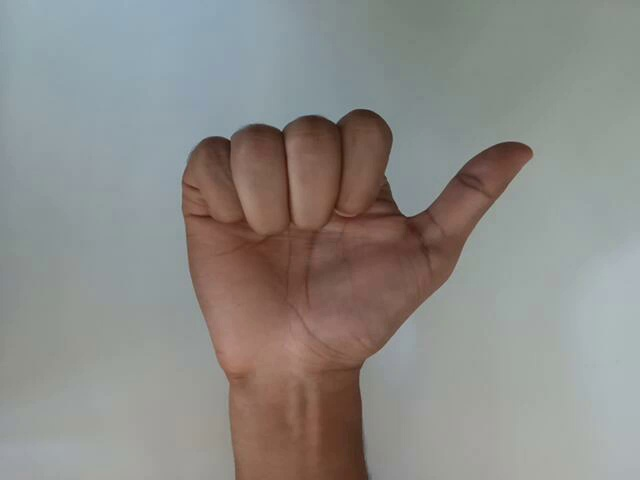
\includegraphics[width=\textwidth]{images/fig33.png}
			\caption{Imagen original}
		\end{subfigure}
		\hfill
		\begin{subfigure}[b]{0.3\textwidth}
			\centering
			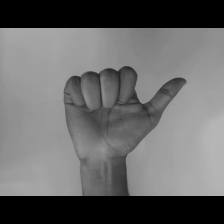
\includegraphics[width=\textwidth]{images/fig34.png}
			\caption{Escala de grises}
		\end{subfigure}
		\hfill
		\begin{subfigure}[b]{0.3\textwidth}
			\centering
			
\includegraphics[width=\textwidth]{images/fig35.png}
			\caption{Segmentación (binarización)}
		\end{subfigure}
		
		\caption{Pipeline de preprocesamiento aplicado en el enfoque basado en imágenes.}
		\label{fig:cnn_dataset}
	\end{figure}
	
	\subsubsection{Cambio de enfoque: uso de landmarks}
	
	Debido a las limitaciones observadas en el enfoque basado en imágenes, se optó por rediseñar la estrategia de construcción del dataset utilizando un enfoque basado en la extracción de características estructurales de la mano mediante landmarks.
	
	Este enfoque permite representar cada seña a partir de la geometría de la mano, eliminando la dependencia de factores como iluminación, color o fondo. Para ello, se empleó MediaPipe Hands, el cual permite detectar la mano y extraer un conjunto de 21 puntos clave que describen su estructura.

	
	Como etapa de validación del nuevo enfoque, se construyó un dataset inicial limitado a las vocales del alfabeto (A, E, I, O, U). Este subconjunto permitió evaluar de manera controlada la viabilidad del uso de landmarks como representación de entrada.
	
	Para este dataset, se capturaron 150 muestras por clase con 5 personas diferentes, considerando variaciones en posición, orientación y distancia de la mano. Los resultados obtenidos con este enfoque mostraron una mejora significativa en la capacidad de generalización del modelo, lo que confirmó la viabilidad de utilizar landmarks como base.
	
	Después de validar este enfoque, se procedió a la construcción del dataset completo del sistema. Para ello, se realizó la captura de datos con la participación de 15 personas diferentes, con el objetivo de introducir variabilidad interusuario y mejorar la capacidad de generalización del modelo.
	
	Cada participante generó aproximadamente 300 muestras por clase, lo que permitió construir un dataset amplio y representativo. Durante la captura, se consideraron distintas condiciones de uso, incluyendo variaciones en iluminación, fondo y posición de la mano, con el fin de simular escenarios reales de operación.
	
	Inicialmente, el proceso de construcción del dataset implicaba capturar imágenes y posteriormente procesarlas para extraer los landmarks. Sin embargo, este enfoque resultaba ineficiente en términos de tiempo y almacenamiento. Entonces se implementó una optimización en el pipeline de captura, en la cual los landmarks eran extraídos directamente en cuanto mediapipe detectaba la mano, evitando el almacenamiento de imágenes intermedias. Este cambio permitió reducir significativamente el volumen de datos almacenados y acelerar el proceso de generación del dataset.
	
	\subsubsection{Estructura final del dataset}
	
	El dataset final se compone de vectores de características derivados de los landmarks de la mano. Cada muestra está representada por un conjunto de coordenadas correspondientes a los 21 puntos clave detectados por MediaPipe, donde cada punto contiene información espacial de su posición.
	
	Inicialmente, cada landmark incluye tres coordenadas $(x, y, z)$, lo que daría lugar a un vector de 63 valores por muestra. Sin embargo, en este trabajo se optó por utilizar únicamente las coordenadas $(x, y)$, generando vectores de dimensión 42.
	
	Esta decisión se fundamenta en varias consideraciones técnicas. En primer lugar, las coordenadas $x$ y $y$ representan la posición bidimensional de los puntos en el plano de la imagen, lo cual es suficiente para capturar la geometría de la mano en el contexto de señas estáticas. La mayoría de las configuraciones relevantes de los dedos y su disposición espacial pueden describirse adecuadamente en dos dimensiones.
	
	En segundo lugar, la coordenada $z$ proporcionada por MediaPipe no corresponde a una medida absoluta de profundidad en unidades físicas, sino a una estimación relativa dependiente del modelo y de la escala de la imagen. Esto introduce variabilidad adicional que puede afectar negativamente la estabilidad del modelo, especialmente en escenarios donde la distancia de la mano respecto a la cámara no está controlada.
	
	La inclusión de la coordenada $z$ incrementa la dimensionalidad del problema sin garantizar una mejora significativa en la capacidad discriminativa del modelo. En sistemas de aprendizaje automático, un aumento innecesario en la dimensionalidad puede incrementar la complejidad del modelo, dificultar el entrenamiento y favorecer el sobreajuste, particularmente cuando la información adicional no aporta características relevantes.
	
	Por estas razones, se decidió reducir la representación a un espacio bidimensional utilizando únicamente las coordenadas $(x, y)$, lo que permitió simplificar el modelo, mejorar la estabilidad del entrenamiento y mantener un desempeño adecuado en la clasificación de señas estáticas.
	
	En consecuencia, cada muestra del dataset se representa como un vector:
	
	\[
	\mathbf{v} = [x_1, y_1, x_2, y_2, \dots, x_{21}, y_{21}] \in \mathbb{R}^{42}
	\]
	
	lo cual representa la entrada del modelo de clasificación utilizado en el sistema.
	
	Los datos fueron almacenados en formato CSV, donde cada fila representa una muestra y cada columna corresponde a una característica del vector, junto con su etiqueta de clase. Esta estructura facilita su uso en procesos de entrenamiento, validación y exportación hacia el modelo final.
	
	En términos generales, el dataset final contiene aproximadamente 300 muestras por persona para cada clase, lo que permite disponer de un volumen suficiente de datos para entrenar modelos robustos y evaluar su desempeño de manera confiable.
	
	Este proceso iterativo de construcción del dataset permitió evolucionar desde un enfoque basado en imágenes, con limitaciones de generalización, hacia un esquema más eficiente y robusto basado en landmarks, el cual constituye la base del sistema propuesto.
	
	\subsection{Extracción de características mediante MediaPipe}
	
	Una de las etapas fundamentales dentro del prototipo propuesto corresponde al
	proceso de extracción de características de la mano a partir de imágenes capturadas
	por la cámara. Esta etapa tiene como objetivo transformar la información visual
	obtenida en la captura en una representación estructurada que pueda ser
	utilizada como entrada para el modelo de clasificación.
	
	Para ello, se empleó MediaPipe Hands, una solución desarrollada por Google para la
	detección y seguimiento de manos mediante técnicas de visión por computadora y
	aprendizaje automático \cite{mediapipe}. Esta herramienta permite detectar la mano
	y obtener un conjunto de 21 puntos clave (\textit{landmarks}) que describen la
	estructura geométrica de la mano dentro de la imagen.
	
	A diferencia de los enfoques basados en imágenes completas, el uso de landmarks
	permite representar cada seña mediante relaciones espaciales entre los puntos de
	la mano, reduciendo la dependencia respecto a factores externos como iluminación,
	color, fondo o resolución de captura. Esto permite disminuir la dimensionalidad
	del problema y centrar el proceso de clasificación en la geometría y disposición
	de los dedos al realizar una seña.
	
	El proceso de extracción de características introduce distintos retos
	relacionados con variaciones de captura, diferencias entre dispositivos,
	consistencia entre entrenamiento e inferencia y estabilidad de los landmarks
	detectados. Por esta razón, fue necesario definir estrategias de representación y
	transformación de los datos que permitieran mantener consistencia en las entradas
	utilizadas por el modelo de clasificación.
	
	En las siguientes subsecciones se describe el funcionamiento general de
	MediaPipe Hands, el proceso de detección y representación de landmarks, la
	transformación de coordenadas, la construcción del vector de características y las
	principales dificultades observadas en la implementación del sistema tanto en
	el entorno experimental como en la aplicación móvil Android.
	
	\subsubsection{Funcionamiento de MediaPipe Hands}
	
	MediaPipe Hands es una solución de visión por computadora desarrollada por Google
	Research para la detección y seguimiento de manos mediante técnicas de aprendizaje
	automático \cite{mediapipeHandsPaper}. Su propósito principal consiste en localizar
	la mano dentro de una imagen y estimar la posición espacial de un conjunto de
	puntos clave (\textit{landmarks}) que describen su estructura geométrica.
	
	A diferencia de enfoques tradicionales basados únicamente en segmentación o
	detección manual de contornos, MediaPipe Hands implementa un pipeline compuesto
	por múltiples etapas optimizadas para operar de manera eficiente en dispositivos
	con recursos limitados. El sistema se encuentra dividido principalmente en dos
	modelos: un detector de palma y un modelo de estimación de landmarks.
	
	La primera etapa corresponde al modelo de detección de palma
	(\textit{Palm Detection Model}), el cual tiene como objetivo localizar la región
	de la imagen donde se encuentra la mano. Este modelo utiliza una arquitectura
	basada en detectores tipo SSD (\textit{Single Shot Detector}), optimizada para la
	detección de palmas en distintas posiciones y orientaciones
	\cite{mediapipeHandsPaper}. En lugar de detectar directamente la mano completa,
	MediaPipe detecta inicialmente la palma debido a que presenta una geometría más
	estable y menos variable respecto a configuraciones complejas de los dedos.
	
	Cuando se detecta la palma, el sistema genera una región de interés
	(\textit{Region of Interest, ROI}) correspondiente a la mano. Esta región es
	recortada y enviada al segundo modelo del pipeline, encargado de estimar la
	posición de los landmarks.
	
	El segundo componente corresponde al modelo de estimación de landmarks
	(\textit{Hand Landmark Model}), el cual funciona como una red neuronal de
	regresión encargada de predecir directamente las coordenadas espaciales de 21
	puntos clave distribuidos sobre diferentes partes de la mano. Estos puntos
	incluyen referencias correspondientes a la muñeca, articulaciones de los dedos y
	puntas de los dedos.
	
	Cada landmark generado por MediaPipe se representa mediante coordenadas
	normalizadas $(x, y, z)$. Las coordenadas $(x, y)$ describen la posición del punto
	dentro del plano de la imagen, mientras que la coordenada $(z)$ representa una
	estimación relativa de profundidad respecto a la cámara. Esta representación
	permite modelar la estructura geométrica de la mano en la realización de una
	seña.
	
	La Figura~\ref{fig:mediapipe_landmarks} muestra la distribución de los 21
	landmarks utilizados por MediaPipe Hands para representar la mano.
	
	\begin{figure}[H]
		\centering
		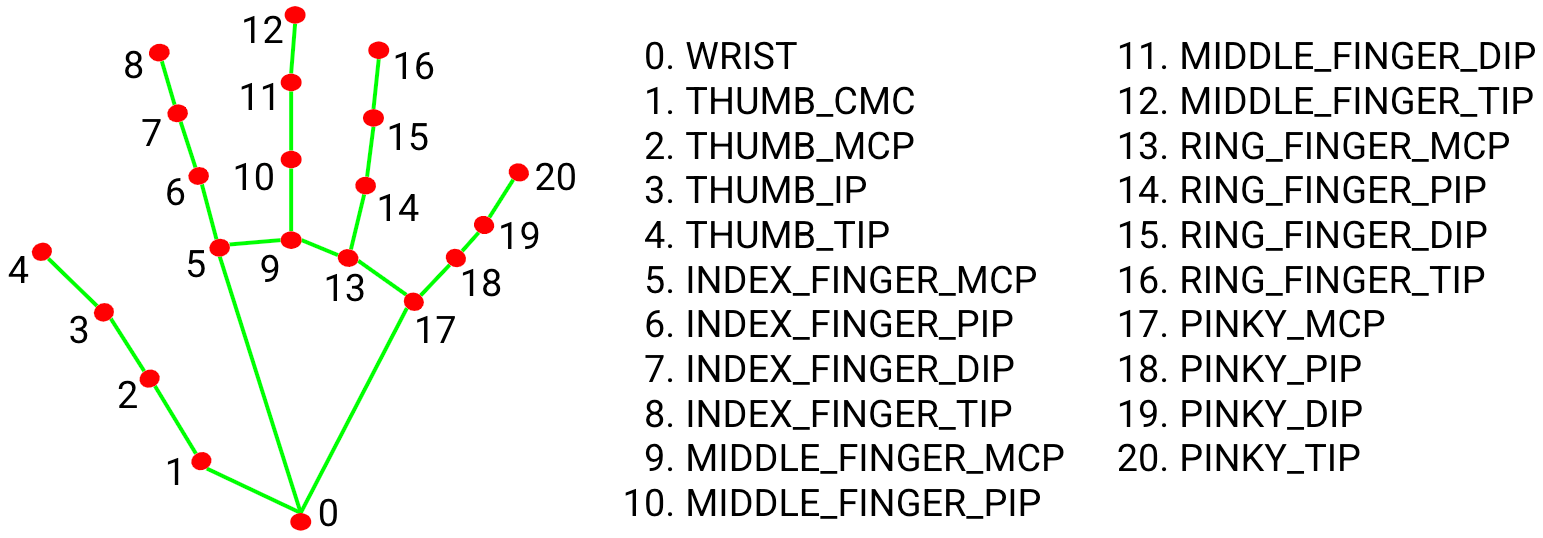
\includegraphics[width=0.7\textwidth]{images/fig23.png}
		\caption{Representación de los 21 landmarks detectados en una mano mediante MediaPipe Hands.\cite{mediapipe_hands}}
		\label{fig:landmarks}
	\end{figure}
	
	Una característica importante de MediaPipe Hands es la incorporación de mecanismos
	de seguimiento temporal (\textit{tracking}). Después de detectar la mano en un
	frame inicial, el sistema reutiliza información espacial obtenida en frames
	anteriores para evitar ejecutar continuamente el detector completo de palma. Este
	enfoque permite reducir significativamente el costo computacional asociado a la
	detección continua y mejora la estabilidad de los landmarks en la captura de
	video.
	
	El pipeline general implementado por MediaPipe Hands puede dividirse en dos
	etapas principales. La primera corresponde al proceso de detección y estimación
	de landmarks, mientras que la segunda se relaciona con el seguimiento temporal
	(\textit{tracking}) utilizado para estabilizar la detección entre frames
	consecutivos.
	
	En la primera etapa, el sistema recibe como entrada un frame capturado por
	la cámara, ejecuta el detector de palma para localizar la mano dentro de la
	imagen y posteriormente genera una región de interés (\textit{ROI}) que es
	procesada por el modelo de regresión encargado de estimar los 21 landmarks de la
	mano.
	
	La Figura~\ref{fig:mediapipe_pipeline_1} muestra el pipeline general utilizado
	por MediaPipe Hands para realizar la detección de palma y la estimación de
	landmarks.
	
	\begin{figure}[H]
		\centering
		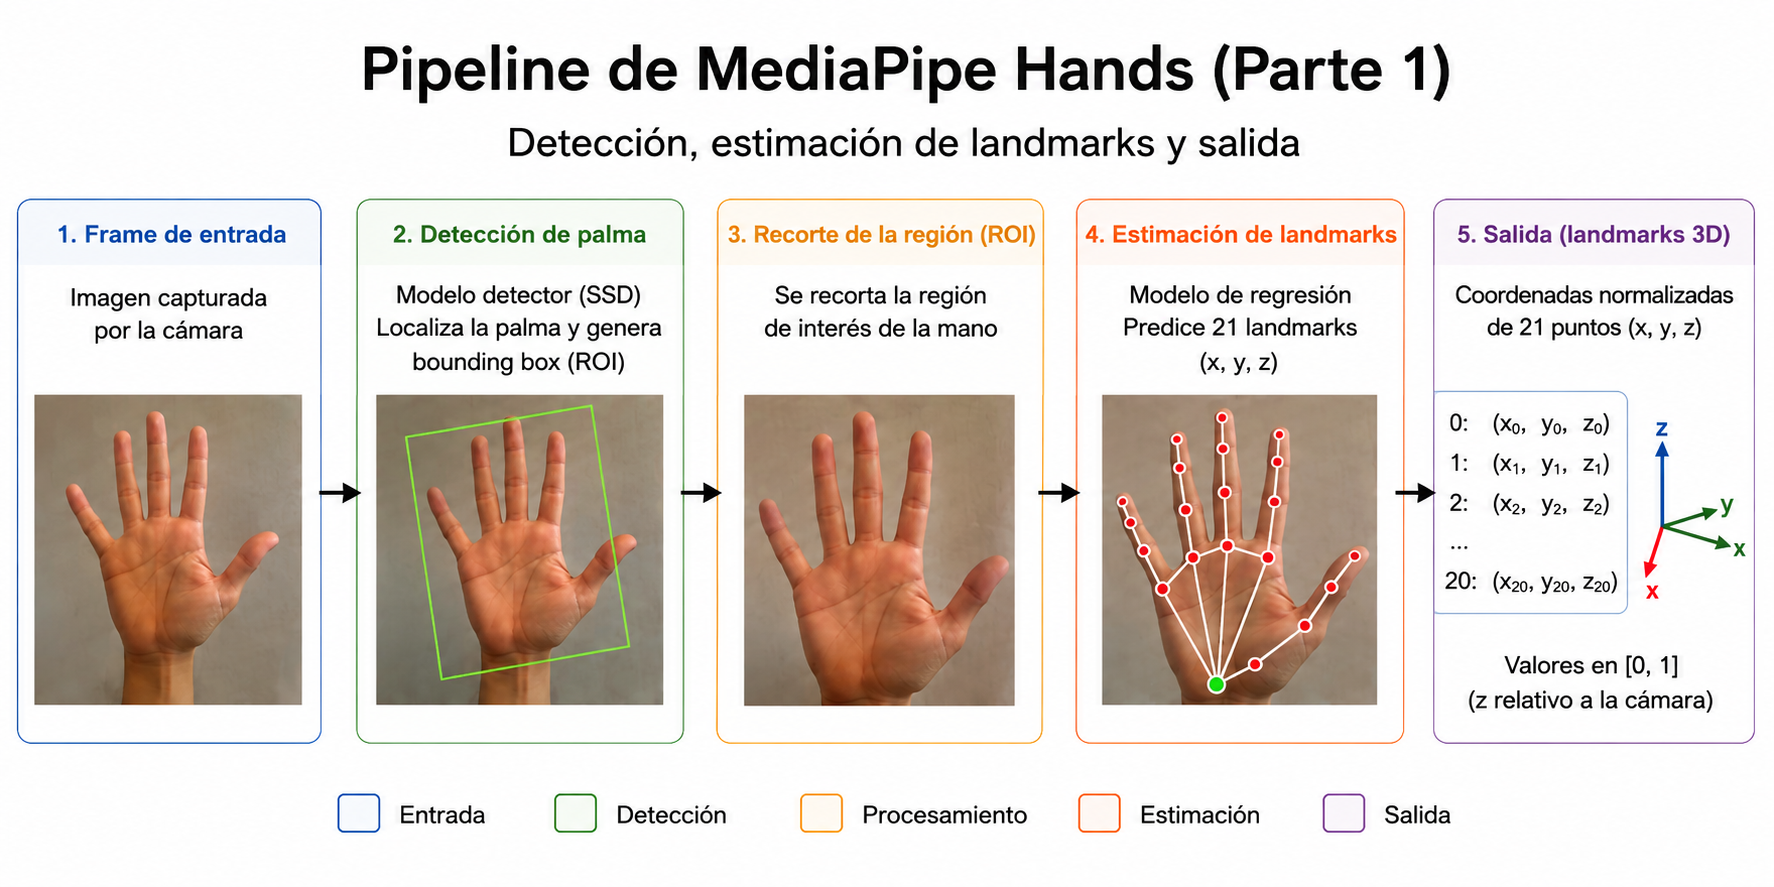
\includegraphics[width=0.95\textwidth]{images/fig43.png}
		\caption{Etapas de detección de palma y estimación de landmarks en MediaPipe Hands.}
		\label{fig:mediapipe_pipeline_1}
	\end{figure}
	
	MediaPipe Hands utiliza mecanismos de seguimiento temporal para
	reutilizar la región de interés detectada en frames previos, evitando ejecutar
	continuamente el detector completo de palma. Este enfoque permite reducir la
	carga computacional y mejorar la estabilidad de los landmarks en secuencias
	continuas de captura.
	
	La Figura~\ref{fig:mediapipe_pipeline_2} muestra el proceso de tracking temporal
	implementado por MediaPipe Hands para mantener la continuidad de los landmarks
	entre frames consecutivos.
	
	\begin{figure}[H]
		\centering
		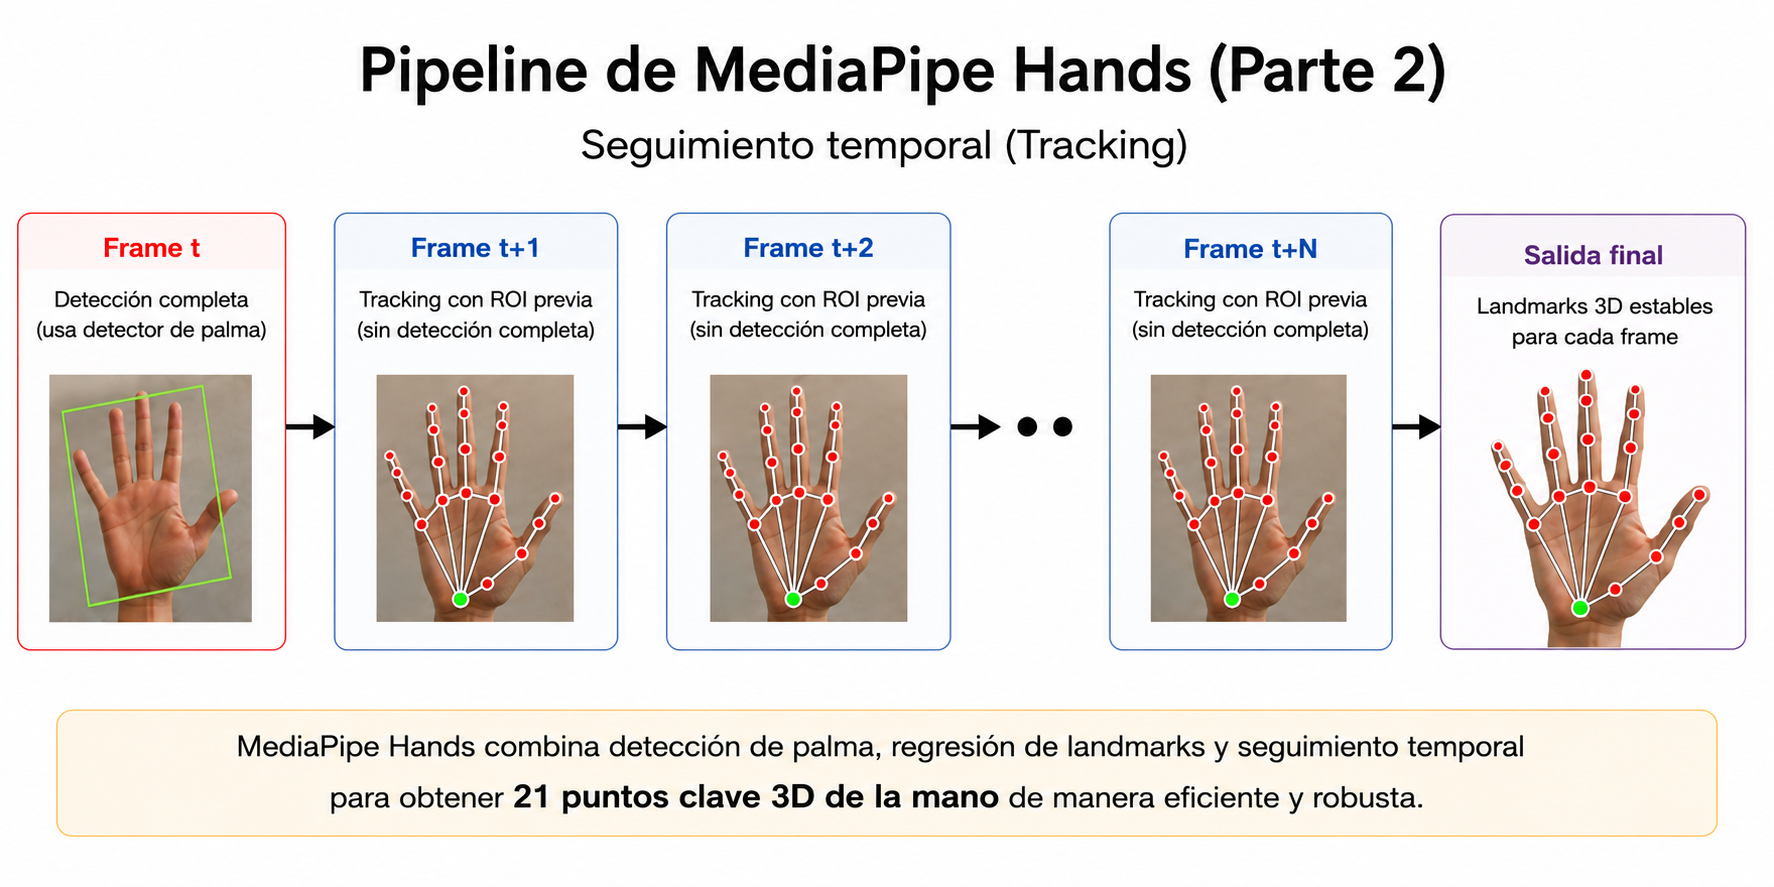
\includegraphics[width=0.95\textwidth]{images/fig44.png}
		\caption{Seguimiento temporal (\textit{tracking}) utilizado por MediaPipe Hands
			para estabilizar la detección de landmarks entre frames consecutivos.}
		\label{fig:mediapipe_pipeline_2}
	\end{figure}
	
	Una de las principales ventajas de este enfoque es que permite representar la mano
	mediante una estructura geométrica compacta en lugar de utilizar imágenes
	completas como entrada del modelo de clasificación. Esto reduce considerablemente
	la dimensionalidad del problema y disminuye la dependencia respecto a factores
	externos como iluminación, color, fondo o resolución de captura.
	
	En este trabajo, MediaPipe Hands se utilizó como componente central
	para la extracción de características tanto en  la construcción del dataset
	como durante la clasificación dentro de la aplicación móvil Android. Cada frame
	capturado por la cámara es transformado en un conjunto de landmarks que
	posteriormente son procesados para construir el vector de características
	utilizado por el modelo de clasificación.
		
	\subsubsection{Detección y representación de landmarks}
	
	Una vez que MediaPipe Hands detecta la presencia de una mano dentro del frame de
	entrada, el sistema obtiene una lista de puntos clave o \textit{landmarks} que
	representan la estructura geométrica de la mano. Cada landmark corresponde a una
	posición específica dentro de la anatomía de la mano, incluyendo la muñeca, las
	articulaciones de los dedos y las puntas de los mismos.
	
	Formalmente, la salida inicial de MediaPipe para una mano puede representarse como
	un conjunto de puntos:
	
	\[
	L = \{(x_0,y_0,z_0), (x_1,y_1,z_1), \ldots, (x_{20},y_{20},z_{20})\}
	\]
	
	donde cada tripleta corresponde a un landmark detectado. Esta representación
	permite sustituir la imagen completa por una descripción estructural de la mano,
	lo cual es adecuado para el reconocimiento de señas estáticas, ya que el
	modelo de clasificación no necesita analizar directamente los píxeles de la
	imagen, sino la disposición espacial de los dedos y articulaciones.
	
	En este trabajo, los landmarks fueron utilizados como base para construir el
	vector de características de entrada del modelo. Para ello, cada frame válido
	debía cumplir con la detección completa de una mano. Cuando MediaPipe no detectaba
	la mano o la detección era incompleta, el frame era descartado para evitar la
	generación de muestras inconsistentes dentro del dataset.
	
	La indexación de los landmarks permite conservar siempre el mismo orden anatómico
	de los puntos detectados. Esto es importante porque el modelo de clasificación
	recibe los datos en una secuencia fija; es decir, el punto correspondiente a la
	muñeca, las articulaciones del pulgar, índice, medio, anular y meñique siempre
	debe ocupar la misma posición dentro del vector de entrada. Si este orden se
	alterara, el modelo recibiría una representación distinta de la mano y podría
	generar clasificaciones incorrectas.
	
	La Figura~\ref{fig:landmarks} muestra la distribución de los 21 puntos
	clave utilizados por MediaPipe Hands. Esta estructura fue tomada como referencia
	para la extracción de características en el entorno experimental y en la aplicación
	móvil Android.
	
	A partir de esta representación inicial, fue necesario aplicar transformaciones
	adicionales para reducir la variabilidad causada por la posición de la mano dentro
	del frame, la distancia respecto a la cámara y las diferencias entre dispositivos
	de captura. Estas transformaciones se describen en las siguientes subsecciones,
	donde se explica el uso de coordenadas relativas, la normalización y la
	construcción final del vector de características.
	
	\subsubsection{Uso de coordenadas relativas}
	
	Inicialmente los landmarks generados por MediaPipe Hands se obtienen como un
	conjunto de coordenadas absolutas normalizadas respecto al tamaño de la imagen de
	entrada. Esto significa que los valores $(x,y)$ de cada punto representan una
	posición específica dentro del frame capturado por la cámara. En consecuencia, si
	la mano cambia de posición dentro de la imagen, las coordenadas de todos los
	landmarks también cambian, aun cuando la configuración geométrica de la seña siga
	siendo la misma.
	
	Este funcionamiento introduce un problema importante para el modelo de
	clasificación, ya que una misma seña puede producir representaciones numéricas muy
	distintas dependiendo de factores como la posición de la mano dentro del frame, la
	distancia respecto a la cámara o el encuadre de captura. Por ejemplo, una seña
	realizada en la parte superior de la imagen generará coordenadas diferentes a la
	misma seña realizada en el centro o en la parte inferior del frame, aun cuando la
	configuración geométrica de la mano permanezca prácticamente igual.
	
	Las coordenadas absolutas corresponden a posiciones medidas
	respecto al sistema de referencia completo de la imagen capturada por la cámara,
	mientras que las coordenadas relativas son calculadas tomando como referencia los
	valores mínimos de las coordenadas $x$ y $y$ del conjunto de landmarks detectados
	en cada frame.
	
	Para reducir esta variabilidad, se implementó una transformación
	basada en coordenadas relativas. En lugar de utilizar directamente las coordenadas
	absolutas proporcionadas por MediaPipe, cada landmark fue transformado tomando
	como referencia los valores mínimos de los puntos detectados en cada frame.
	
	Para ello, primero se obtuvieron los valores mínimos de las coordenadas $x$ y
	$y$ entre los 21 landmarks detectados:
	
	\[
	x_{min} = \min(x_0,x_1,\ldots,x_{20})
	\]
	
	\[
	y_{min} = \min(y_0,y_1,\ldots,y_{20})
	\]
	
	Posteriormente, cada landmark fue transformado restando dichos valores mínimos a
	sus coordenadas originales:
	
	\[
	x_i' = x_i - x_{min}
	\]
	
	\[
	y_i' = y_i - y_{min}
	\]
	
	De esta forma todos los landmarks pasan a representarse respecto al punto más
	cercano al origen dentro del conjunto detectado. Esta transformación permite que
	la representación de la mano conserve principalmente su geometría relativa y no su
	posición absoluta dentro de la imagen.
	
	La principal ventaja de este enfoque es la reducción de variaciones relacionadas
	con translación espacial. Aunque la mano cambie de posición dentro del frame, las
	distancias relativas entre landmarks permanecen estables, permitiendo que el
	modelo de clasificación se enfoque en la configuración geométrica de la seña y no
	en su ubicación dentro de la imagen.
	
	En las pruebas experimentales se observó que el uso de coordenadas absolutas
	provocaba una disminución significativa en la estabilidad del modelo, ya que
	pequeños desplazamientos de la mano generaban variaciones importantes en los
	vectores de entrada. En contraste, el uso de coordenadas relativas permitió
	obtener representaciones más consistentes entre distintas capturas.
	
	Para comprender el efecto de las coordenadas absolutas y relativas, considérese
	el siguiente ejemplo simplificado. Supóngase que una misma seña es realizada en
	dos posiciones distintas dentro del frame capturado por la cámara.
	
	En el primer caso, un landmark puede ubicarse en la posición:
	
	\[
	(x,y)=(0.20,0.30)
	\]
	
	mientras que en una segunda captura, debido únicamente al desplazamiento de la
	mano dentro de la imagen, el mismo landmark puede aparecer en:
	
	\[
	(x,y)=(0.55,0.65)
	\]
	
	Aunque la configuración geométrica de la mano sea exactamente la misma, las
	coordenadas absolutas cambian considerablemente debido a la nueva posición de la
	mano dentro del frame. Esto provoca que el modelo reciba representaciones
	numéricas distintas para una misma seña.
	
	Para reducir este problema, se utilizaron coordenadas relativas calculadas a
	partir de los valores mínimos del conjunto de landmarks detectados. Supóngase que
	para una captura determinada se obtienen los siguientes valores mínimos:
	
	\[
	x_{min}=0.20
	\]
	
	\[
	y_{min}=0.30
	\]
	
	Entonces, cada landmark se transforma mediante:
	
	\[
	x_i' = x_i - x_{min}
	\]
	
	\[
	y_i' = y_i - y_{min}
	\]
	
	Por ejemplo, si un landmark original posee coordenadas:
	
	\[
	(x_i,y_i)=(0.35,0.50)
	\]
	
	la transformación relativa produce:
	
	\[
	(x_i',y_i')=(0.35-0.20,\;0.50-0.30)=(0.15,0.20)
	\]
	
	Ahora considérese una segunda captura donde la mano aparece desplazada dentro del
	frame, pero mantiene exactamente la misma geometría. Supóngase que el landmark
	equivalente posee coordenadas absolutas:
	
	\[
	(x_i,y_i)=(0.70,0.85)
	\]
	
	y que los nuevos mínimos del conjunto corresponden a:
	
	\[
	x_{min}=0.55
	\]
	
	\[
	y_{min}=0.65
	\]
	
	Aplicando nuevamente la transformación relativa:
	
	\[
	(x_i',y_i')=(0.70-0.55,\;0.85-0.65)=(0.15,0.20)
	\]
	
	Puede observarse que, aunque las coordenadas absolutas son completamente
	distintas, las coordenadas relativas resultantes permanecen iguales. Esto permite
	que el modelo de clasificación se enfoque principalmente en la configuración
	geométrica de la mano y no en la posición específica donde la seña fue realizada
	dentro de la imagen.
	
	\begin{figure}[H]
		\centering
		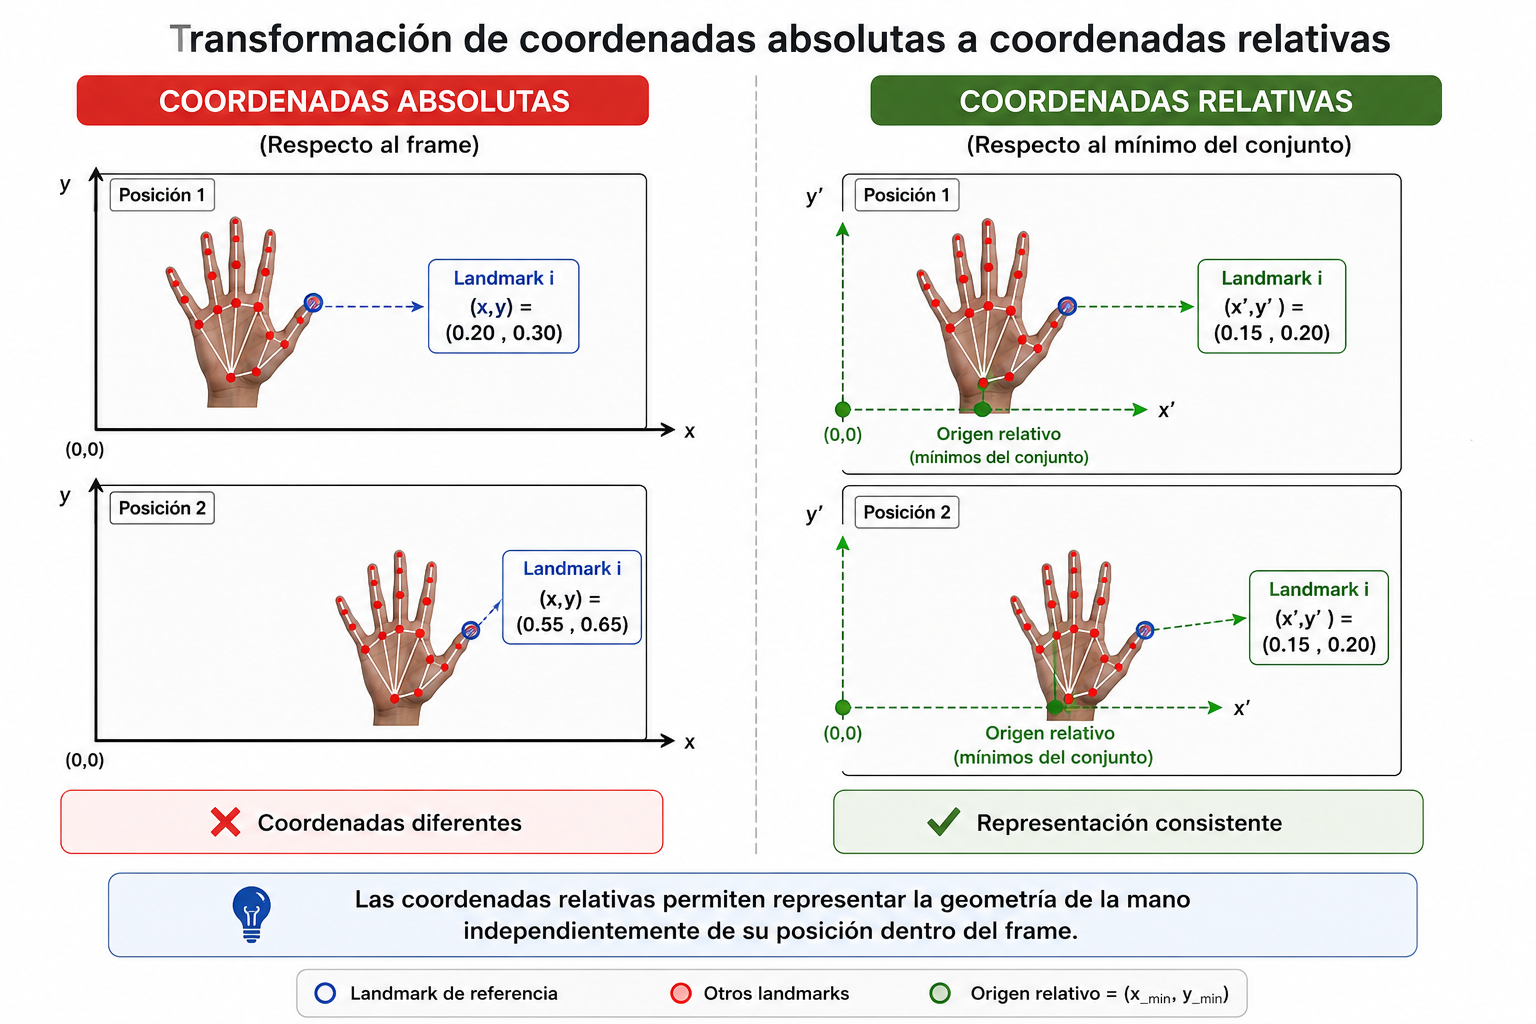
\includegraphics[width=0.8\textwidth]{images/fig45.png}
		\caption{Comparación entre coordenadas absolutas y coordenadas relativas.
			Las coordenadas absolutas dependen de la posición de la mano dentro del
			frame, mientras que las coordenadas relativas permiten conservar la
			geometría de la seña independientemente de su ubicación espacial.}
		\label{fig:absolute_vs_relative}
	\end{figure}
	
	Otro aspecto importante corresponde al uso de la coordenada de profundidad
	$(z)$ proporcionada por MediaPipe Hands. Inicialmente, cada landmark contiene tres
	coordenadas espaciales $(x,y,z)$, lo que permitiría representar cada muestra
	mediante un vector de 63 características. El desarrollo del
	prototipo se decidió utilizar únicamente las coordenadas $(x,y)$ para construir el
	vector de entrada del modelo.
	
	Esta decisión se tomó debido a que la coordenada $z$ generada por MediaPipe no
	corresponde a una medida absoluta de profundidad en unidades físicas reales, sino
	a una estimación relativa dependiente del modelo y de la escala de captura
	\cite{mediapipeHandsPaper}. Como consecuencia, pequeñas variaciones en distancia,
	orientación o posición respecto a la cámara podían introducir cambios importantes
	en los valores de profundidad.
	
	En las realizadas, se observó que la incorporación de la coordenada
	$z$ aumentaba la variabilidad de los datos sin aportar mejoras significativas en
	la capacidad de discriminación del modelo para señas estáticas. Además, el uso de
	la coordenada de profundidad incrementaba la dimensionalidad del problema,
	generando vectores más grandes y aumentando la complejidad del proceso de
	entrenamiento.
	
	Por esta razón, se optó por utilizar únicamente coordenadas bidimensionales,
	permitiendo representar cada muestra mediante un vector de 42 características:
	
	\[
	v =
	[x_0',y_0',
	x_1',y_1',
	\ldots,
	x_{20}',y_{20}']
	\in \mathbb{R}^{42}
	\]
	
	El uso de coordenadas relativas resultó fundamental para mantener
	consistencia entre el entorno experimental y la aplicación móvil Android, ya que
	ambos entornos presentan diferencias relacionadas con resolución, orientación de
	captura, cámara utilizada y procesamiento interno de imágenes. La utilización de
	una representación geométrica relativa permitió disminuir parcialmente el impacto
	de estas variaciones sobre el comportamiento del modelo de clasificación.
	
	\subsubsection{Normalización de landmarks}
	
	Aunque el uso de coordenadas relativas permitió reducir la variabilidad asociada
	a la posición de la mano dentro del frame, todavía existían diferencias
	importantes relacionadas con la escala de captura. Estas variaciones podían
	originarse debido a cambios en la distancia entre la mano y la cámara, distintos
	tamaños de mano entre usuarios o diferencias en el encuadre durante la captura.
	
	Por ejemplo, una misma seña realizada cerca de la cámara podía generar distancias
	entre landmarks considerablemente mayores que la misma seña realizada a una mayor
	distancia, aun cuando la configuración geométrica de la mano permaneciera
	prácticamente igual. Como consecuencia, el modelo de clasificación recibía
	vectores numéricos con escalas distintas para una misma clase.
	
	Para reducir este problema, se implementó un proceso de normalización aplicado
	sobre las coordenadas relativas obtenidas previamente. El objetivo de esta etapa
	consiste en mantener una representación más consistente de la geometría de la
	mano independientemente de su tamaño aparente dentro de la imagen.
	
	Inicialmente, para cada frame se calcularon el ancho y alto del conjunto de
	landmarks detectados:
	
	\[
	width = \max(x') - \min(x')
	\]
	
	\[
	height = \max(y') - \min(y')
	\]
	
	Posteriormente, cada coordenada relativa fue normalizada respecto a estas
	dimensiones:
	
	\[
	x_i'' = \frac{x_i'}{width}
	\]
	
	\[
	y_i'' = \frac{y_i'}{height}
	\]
	
	Esta transformación permite que las distancias entre landmarks sean expresadas en
	función del tamaño de la propia mano detectada y no del tamaño absoluto dentro
	del frame capturado por la cámara.
	
	Para comprender el efecto de la normalización, considérese el siguiente ejemplo
	simplificado. Supóngase que una misma seña es realizada a diferentes distancias
	respecto a la cámara.
	
	Después de aplicar la transformación a coordenadas relativas, un landmark de una
	captura cercana podría representarse mediante:
	
	\[
	(x_i',y_i')=(0.40,0.60)
	\]
	
	mientras que para una captura más alejada el mismo landmark podría aparecer como:
	
	\[
	(x_i',y_i')=(0.20,0.30)
	\]
	
	Aunque ambas capturas representan exactamente la misma configuración geométrica
	de la mano, las distancias entre landmarks son distintas debido al cambio de
	escala provocado por la distancia respecto a la cámara.
	
	Supóngase ahora que para la primera captura se obtiene:
	
	\[
	width = 0.80
	\]
	
	\[
	height = 1.20
	\]
	
	Aplicando la normalización:
	
	\[
	x_i'' = \frac{x_i'}{width}
	\]
	
	\[
	y_i'' = \frac{y_i'}{height}
	\]
	
	se obtiene:
	
	\[
	(x_i'',y_i'')=
	\left(
	\frac{0.40}{0.80},
	\frac{0.60}{1.20}
	\right)
	=
	(0.50,0.50)
	\]
	
	Ahora considérese la segunda captura, correspondiente a una mano más alejada de
	la cámara. Supóngase que para este caso se obtiene:
	
	\[
	width = 0.40
	\]
	
	\[
	height = 0.60
	\]
	
	Aplicando nuevamente la normalización:
	
	\[
	(x_i'',y_i'')=
	\left(
	\frac{0.20}{0.40},
	\frac{0.30}{0.60}
	\right)
	=
	(0.50,0.50)
	\]
	
	Puede observarse que, aunque las coordenadas relativas originales poseen escalas
	distintas, la normalización permite obtener representaciones equivalentes para
	una misma seña. Esto reduce la dependencia respecto al tamaño aparente de la
	mano dentro del frame y favorece que el modelo de clasificación se enfoque
	principalmente en la geometría de la seña.
	
	La Figura~\ref{fig:landmark_normalization} muestra un ejemplo conceptual del
	proceso de normalización aplicado sobre los landmarks detectados.
	
	\begin{figure}[H]
		\centering
		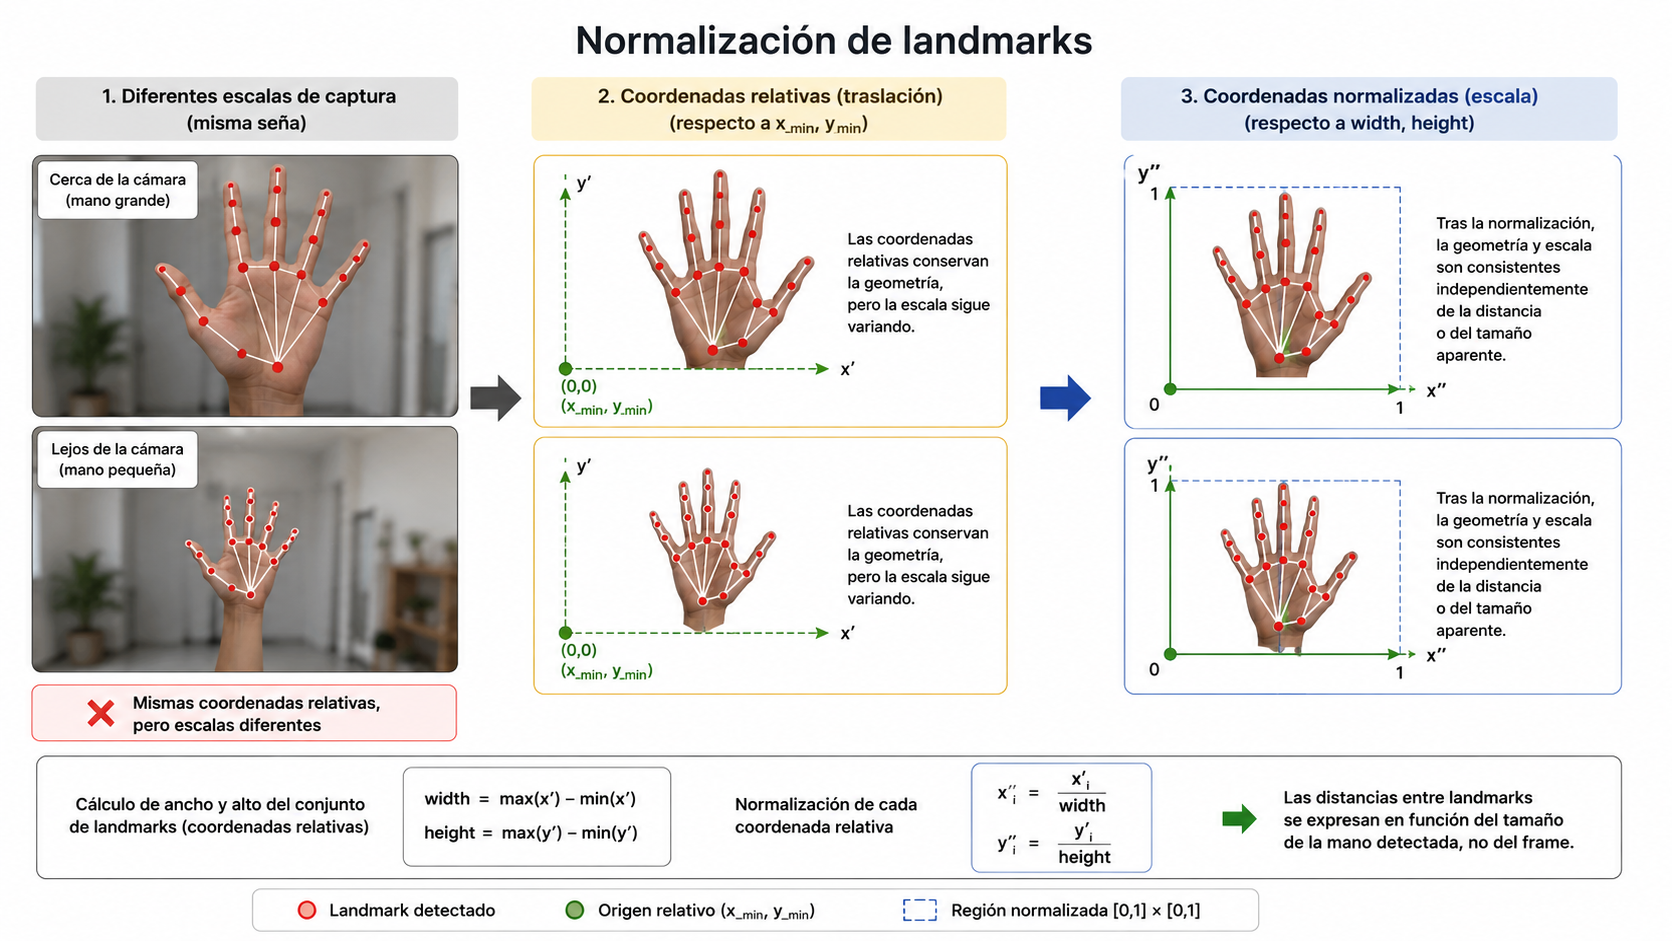
\includegraphics[width=1\textwidth]{images/fig46.png}
		\caption{Proceso conceptual de normalización aplicado a los landmarks.
			La geometría relativa de la mano se conserva independientemente de la
			escala de captura.}
		\label{fig:landmark_normalization}
	\end{figure}
	
	Una de las principales ventajas de este enfoque es la reducción de variaciones
	causadas por diferencias de escala entre capturas. Gracias a ello, el modelo de
	clasificación puede enfocarse principalmente en la forma y disposición de los
	dedos, disminuyendo la influencia de factores relacionados con distancia o tamaño
	aparente de la mano.
	
	Se observó que la ausencia de normalización
	provocaba inconsistencias importantes entre el entorno de entrenamiento y la
	inferencia dentro de dispositivos móviles Android. Diferencias relacionadas con
	resolución de cámara, tamaño del frame y procesamiento interno de imágenes podían
	modificar significativamente los valores de entrada recibidos por el modelo.
	
	La normalización permitió reducir parcialmente estas diferencias, favoreciendo
	una representación más estable y consistente entre distintos dispositivos y
	entornos de captura. Esto es importante en la integración
	del sistema dentro de la aplicación móvil, donde pequeñas variaciones en la
	captura podían afectar directamente la estabilidad de las predicciones generadas
	por el modelo de clasificación.
	
	\subsubsection{Construcción del vector de características}
	
	Ya obtenidos los landmarks de la mano y aplicadas las etapas de
	transformación a coordenadas relativas y normalización, fue necesario construir
	una representación numérica adecuada para ser utilizada como entrada del modelo
	de clasificación.
	
	En aprendizaje automático, los modelos de clasificación requieren que la
	información de entrada sea representada mediante vectores numéricos de dimensión
	fija \cite{goodfellow2016deep}. Por esta razón, las coordenadas procesadas de los
	landmarks fueron organizadas en una estructura unidimensional denominada vector
	de características.
	
	Como se describió anteriormente, MediaPipe Hands proporciona un conjunto de 21
	landmarks para cada mano detectada. Debido a que únicamente se utilizaron las
	coordenadas bidimensionales normalizadas $(x,y)$, cada landmark quedó definido
	mediante dos valores numéricos:
	
	\[
	(x_i'',y_i'')
	\]
	
	donde:
	
	\[
	i \in \{0,1,2,\dots,20\}
	\]
	
	Posteriormente, todas las coordenadas fueron concatenadas siguiendo un orden
	constante basado en la numeración original de MediaPipe Hands. El vector final de
	entrada utilizado por el sistema quedó definido como:
	
	\[
	v =
	[x_0'',y_0'',
	x_1'',y_1'',
	\ldots,
	x_{20}'',y_{20}'']
	\in \mathbb{R}^{42}
	\]
	
	Así cada muestra del dataset quedó representada mediante un vector de
	42 características numéricas.
	
	Para ilustrar este proceso, considérese el siguiente ejemplo simplificado.
	Supóngase que después de aplicar el preprocesamiento se obtienen las siguientes
	coordenadas normalizadas para algunos landmarks:
	
	\[
	(x_0'',y_0'')=(0.00,0.00)
	\]
	
	\[
	(x_1'',y_1'')=(0.12,0.08)
	\]
	
	\[
	(x_2'',y_2'')=(0.20,0.15)
	\]
	
	\[
	\vdots
	\]
	
	\[
	(x_{20}'',y_{20}'')=(0.91,0.74)
	\]
	
	Entonces, el vector de entrada generado para el modelo tendría la forma:
	
	\[
	v =
	[
	0.00,0.00,
	0.12,0.08,
	0.20,0.15,
	\ldots,
	0.91,0.74
	]
	\]
	
	Este vector corresponde a la representación final utilizada como entrada del
	modelo de clasificación en las etapas de entrenamiento e inferencia.
	
	Mantener un orden fijo en la concatenación de coordenadas resulta
	fundamental, ya que el modelo aprende patrones espaciales específicos asociados
	a cada posición dentro del vector. Una alteración en el orden de los landmarks
	provocaría inconsistencias entre las muestras utilizadas en entrenamiento e
	inferencia, afectando directamente el desempeño del clasificador.
	
	Una de las principales ventajas de esta representación es la reducción
	significativa de dimensionalidad respecto al uso de imágenes completas como
	entrada. Mientras que una imagen RGB de resolución moderada puede contener
	cientos de miles de valores numéricos, el enfoque basado en landmarks permite
	describir la geometría de la mano utilizando únicamente 42 características.
	
	Esta reducción de dimensionalidad disminuye el costo computacional del sistema y
	favorece la ejecución dentro de dispositivos móviles con recursos
	limitados. Además, permite que el modelo de clasificación se enfoque
	principalmente en la estructura geométrica de la mano en lugar de depender de
	información visual relacionada con iluminación, color o fondo.
	
	\subsubsection{Pipeline de extracción durante la captura}
	
	El proceso de generación del dataset fue dividido en múltiples etapas con el
	objetivo de mantener separadas las tareas relacionadas con captura,
	preprocesamiento, validación y entrenamiento del modelo. Esta separación permitió
	facilitar el control de las muestras generadas, así como mantener consistencia
	entre el entorno experimental y el sistema de inferencia implementado
	posteriormente en Android.
	
	El pipeline general utilizado en la construcción del dataset puede resumirse
	de la siguiente manera:
	
	\[
	\text{Cámara}
	\rightarrow
	\text{Frame}
	\rightarrow
	\text{MediaPipe Hands}
	\rightarrow
	\text{Landmarks}
	\rightarrow
	\text{Coordenadas relativas}
	\]
	
	\[
	\texttt{data.pickle}
	\rightarrow
	\text{Normalización}
	\rightarrow
	\text{Vector de entrada}
	\rightarrow
	\text{Entrenamiento}
	\]
	
	Inicialmente, se desarrolló un módulo de captura encargado de obtener imágenes
	directamente desde la cámara utilizando OpenCV. En esta etapa, el sistema
	mostraba al usuario la letra correspondiente que debía realizar, así como
	indicaciones relacionadas con el inicio, repetición o finalización de la captura.
	
	Con la finalidad de reducir redundancia entre muestras consecutivas, se implementó
	un mecanismo de muestreo basado en intervalos de frames. En lugar de almacenar
	todos los frames capturados por la cámara, únicamente se seleccionaba un frame
	cada cierto número de iteraciones.
	
	En el sistema implementado se utilizó un valor de:
	
	\[
	FRAME\_SKIP = 15
	\]
	
	Esto permitió reducir la cantidad de imágenes prácticamente idénticas dentro del
	dataset, favoreciendo una mayor variabilidad entre muestras consecutivas y
	disminuyendo redundancia temporal en la captura.
	
	Despues de  seleccionar el frame correspondiente, la imagen era procesada mediante
	MediaPipe Hands para detectar la presencia de la mano y extraer los 21 landmarks
	asociados. En esta etapa únicamente se consideraban muestras válidas cuando
	MediaPipe detectaba correctamente una mano y generaba la totalidad de landmarks
	esperados.
	
	Posteriormente, sobre los landmarks detectados se aplicaba la transformación a
	coordenadas relativas descrita anteriormente. Para ello, se calculaban los valores
	mínimos de las coordenadas $x$ y $y$ del conjunto detectado y posteriormente se
	desplazaban todos los puntos respecto a dichos valores mínimos.
	
	Es importante señalar que en esta etapa todavía no se aplicaba la
	normalización por escala. El archivo \texttt{data.pickle} almacenaba únicamente
	las coordenadas relativas generadas a partir de MediaPipe Hands. Esta decisión
	permitió mantener separadas las etapas de extracción y entrenamiento,
	facilitando modificaciones posteriores en el proceso de normalización sin
	necesidad de reconstruir completamente el dataset.
	
	Cada muestra válida era almacenada junto con su etiqueta correspondiente dentro
	de una estructura serializada mediante \texttt{pickle}. 
	
	Para el almacenamiento del dataset se utilizó el formato serializado
	\texttt{pickle} de Python. Esta decisión permitió almacenar de manera directa
	las estructuras de datos generadas en la extracción de landmarks,
	incluyendo vectores de características y etiquetas asociadas a cada muestra.
	
	El dataset final fue organizado mediante una estructura compuesta
	principalmente por dos elementos:
	
	\[
	\texttt{data}
	\]
	
	correspondiente a los vectores de características extraídos de los landmarks, y:
	
	\[
	\texttt{labels}
	\]
	
	correspondiente a las etiquetas asociadas a cada seña.
	
	Conceptualmente, la estructura almacenada mediante \texttt{pickle} puede
	representarse de la siguiente manera:
	
	\begin{verbatim}
		{
			"data": [
			[0.00,0.00,0.12,0.08,...,0.91,0.74],
			[0.00,0.00,0.10,0.07,...,0.89,0.72],
			...
			],
			
			"labels": [
			"A",
			"A",
			...
			]
		}
	\end{verbatim}
	
	El uso de \texttt{pickle} facilitó la manipulación del dataset en las etapas
	de entrenamiento y experimentación, permitiendo cargar nuevamente los datos sin
	necesidad de reprocesar las imágenes originales. Además, este enfoque permitió
	mantener la estructura original de listas y vectores numéricos utilizada en 
	el desarrollo del sistema.
	
	Aunque formatos como CSV también podían utilizarse para almacenar los vectores
	de características, \texttt{pickle} ofreció mayor flexibilidad en la etapa
	experimental, específicamente al trabajar con estructuras de datos generadas
	directamente en Python.
	
	Por ejemplo, utilizando \texttt{pickle} era posible recuperar directamente el
	dataset completo mediante:
	
	\begin{verbatim}
		data_dict["data"]
		data_dict["labels"]
	\end{verbatim}
	
	sin necesidad de realizar conversiones adicionales de formato o procesamiento de
	columnas como ocurre normalmente en archivos CSV.
	
	
	
	En las primeras pruebas experimentales se observó un comportamiento
	inconsistente en el proceso de clasificación relacionado con la orientación horizontal de
	las muestras. En particular, el modelo mostraba dificultades para reconocer
	correctamente ciertas señas cuando la representación espacial de la mano aparecía
	invertida horizontalmente respecto a las muestras utilizadas en el
	entrenamiento.
	
	Después de analizar el comportamiento del sistema, se identificó que parte de
	esta variación estaba relacionada con el uso de cámaras frontales y visualización
	tipo \textit{selfie}, donde las capturas podían presentar inversiones
	horizontales respecto a las imágenes originales utilizadas para generar el
	dataset.
	
	Para reducir este problema, durante la generación del dataset se implementó una
	estrategia de aumentación basada en reflejo horizontal.
	
	Esta estrategia permitió incrementar la variabilidad espacial del dataset y
	favoreció que el modelo aprendiera representaciones más robustas frente a cambios
	de orientación horizontal en la inferencia. Esto también permitió reducir
	las diferencias observadas entre distintas configuraciones de captura en las
	pruebas realizadas tanto en computadora como en dispositivos móviles Android.
	
	En la etapa de entrenamiento, los landmarks almacenados en
	\texttt{data.pickle} eran cargados nuevamente para aplicar la normalización por
	escala y construir finalmente el vector de entrada utilizado por el modelo de
	clasificación.
	
	La separación entre la etapa de extracción y la etapa de entrenamiento permitió
	reutilizar el mismo dataset para experimentar con diferentes estrategias de
	normalización, arquitecturas de clasificación y configuraciones de entrenamiento
	sin necesidad de repetir nuevamente el proceso completo de captura de imágenes y
	extracción de landmarks.
	
	Esto ayudo a mantener un pipeline más flexible y facilitó
	la reproducción del mismo flujo de procesamiento en la inferencia en
	dispositivos Android, donde se necesitaron aplicar exactamente las mismas
	transformaciones antes de ejecutar el modelo TensorFlow Lite.
	
	Al proceso de construcción del dataset se basaba en almacenar
	imágenes capturadas desde cámara para posteriormente ejecutar la extracción de
	landmarks mediante un proceso independiente. Se ayudo a la 
	validación manual de muestras y realizar múltiples pruebas relacionadas con
	preprocesamiento y extracción de características.
	
	Posteriormente se observó que almacenar imágenes completas
	incrementaba considerablemente el volumen de datos generado y aumentaba el tiempo
	necesario para procesar el dataset.
	
	Es así que en etapas posteriores del desarrollo se adoptó un enfoque
	basado en extracción directa de landmarks en la captura, evitando el
	almacenamiento innecesario de imágenes intermedias.
	
	\subsubsection{Pruebas preliminares de inferencia en entorno de escritorio}
	
	Buscando validar el funcionamiento general del pipeline de reconocimiento antes de su integración en dispositivos móviles, se realizaron diversas pruebas preliminares de inferencia en un entorno de escritorio utilizando una cámara web convencional, MediaPipe Hands y modelos exportados en formato TensorFlow Lite.
	
	Estas pruebas permitieron verificar la correcta detección de la mano, la extracción de landmarks, la generación del vector de características y la ejecución del modelo entrenado mediante inferencia continua. Asimismo, sirvieron para analizar el comportamiento del sistema bajo distintas estrategias de normalización y preprocesamiento de datos, las cuales influyen directamente en la estabilidad y consistencia de las predicciones.
	
	En esta etapa se desarrollaron tres variantes principales del pipeline de inferencia, cada una con diferencias en la forma en que se normalizaban las coordenadas obtenidas por MediaPipe antes de ser enviadas al modelo de clasificación.
	
	La primera variante utilizó una normalización relativa basada únicamente en el desplazamiento respecto al valor mínimo de las coordenadas de la mano, conservando las diferencias espaciales originales entre los landmarks. En este enfoque, cada coordenada era transformada mediante la resta del valor mínimo detectado en los ejes X y Y.
	
	Posteriormente, se implementó una segunda variante que incorporó una normalización basada en escala utilizando el valor máximo entre el ancho y el alto de la mano detectada. Este enfoque buscaba reducir el efecto producido por cambios de distancia entre la mano y la cámara, manteniendo una proporción geométrica uniforme en la inferencia.
	
	Para finalizar se desarrolló una tercera variante orientada específicamente a la integración móvil en Android. En este caso, las coordenadas fueron normalizadas de manera independiente para cada eje, utilizando el ancho de la mano para las coordenadas X y el alto para las coordenadas Y. Aunque esta estrategia modificaba parcialmente la proporción geométrica original de la mano, en las pruebas mostró un comportamiento considerablemente más estable, particularmente bajo variaciones de orientación, distancia y resolución de captura.
	
	
	Para analizar el comportamiento práctico de las distintas variantes de inferencia desarrolladas en esta etapa, se realizaron pruebas controladas considerando variaciones comunes durante el uso del sistema, tales como cambios de distancia entre la mano y la cámara, diferencias de iluminación, variaciones de fondo y ligeras modificaciones en la orientación de la mano.
	
	Las pruebas fueron ejecutadas utilizando cuatro señas representativas con distintos niveles de complejidad visual. La seña ``A'' fue utilizada como referencia de baja complejidad debido a su forma estable y compacta; la seña ``C'' representó una complejidad intermedia al requerir una curvatura más definida de la mano; mientras que las señas ``S'' y ``U'' fueron consideradas de mayor dificultad debido a la similitud estructural con otras configuraciones de mano y a la necesidad de mantener separaciones precisas entre dedos.
	
	En las pruebas se evaluó principalmente la estabilidad de las predicciones, la consistencia del reconocimiento, el comportamiento bajo cambios de escala y orientación, así como la robustez general del pipeline de inferencia antes de su integración en Android.
	
	Con el propósito de evaluar el comportamiento preliminar de las distintas variantes de inferencia desarrolladas en esta etapa, se realizaron pruebas controladas en un entorno de escritorio utilizando una cámara web convencional, MediaPipe Hands y modelos exportados en formato TensorFlow Lite. 
	
	Las pruebas fueron ejecutadas considerando distintas estrategias de normalización aplicadas sobre los 21 landmarks detectados por MediaPipe antes de ser enviados al modelo de clasificación. Cada variante representa una evolución progresiva del pipeline de inferencia, permitiendo analizar el efecto de distintas representaciones geométricas de la mano sobre la estabilidad del reconocimiento.
	
	Para esta primera fase se seleccionaron cuatro señas representativas con distintos niveles de complejidad visual: ``A'', ``C'', ``S'' y ``U''. La seña ``A'' fue utilizada como referencia de baja complejidad debido a su configuración estable y compacta; la seña ``C'' representó una complejidad intermedia al requerir una curvatura más definida de la mano; mientras que ``S'' y ``U'' fueron consideradas señas de mayor dificultad debido a la similitud estructural con otras configuraciones de mano y a la necesidad de mantener separaciones precisas entre dedos.
	
	Cada seña fue ejecutada diez veces consecutivas por variante, calculando posteriormente un promedio aproximado de confianza a partir de las predicciones obtenidas en la inferencia. Las pruebas se realizaron a una distancia aproximada de 50 cm respecto al lente de la cámara bajo condiciones de iluminación desfavorables, utilizando únicamente una fuente de luz lateral proveniente de una lámpara de escritorio. Asimismo, el entorno presentaba una cantidad considerable de elementos visuales en el fondo, generando ruido visual adicional en la detección de la mano.
	
	Estas condiciones fueron seleccionadas intencionalmente debido a que representan uno de los escenarios más complejos para el sistema, permitiendo observar el comportamiento de cada variante bajo situaciones menos controladas antes de continuar con pruebas en ambientes mejor iluminados.
	
	\rowcolors{2}{rowblue}{white}
	
	\small
	\renewcommand{\arraystretch}{1.15}
	
	\begin{longtable}{|p{1cm}|p{2cm}|p{1.2cm}|p{1.2cm}|p{1.2cm}|p{1.2cm}|p{4.8cm}|}
		\caption{Resultados preliminares de las variantes de inferencia bajo condiciones de iluminación complejas} \\
		\hline
		\rowcolor{headerblue}
		\headercell{Variante} &
		\headercell{Estrategia de normalización} &
		\headercell{Seña A} &
		\headercell{Seña C} &
		\headercell{Seña S} &
		\headercell{Seña U} &
		\headercell{Observaciones generales} \\
		\hline
		\endfirsthead
		
		\hline
		\rowcolor{headerblue}
		\headercell{Variante} &
		\headercell{Estrategia de normalización} &
		\headercell{Seña A} &
		\headercell{Seña C} &
		\headercell{Seña S} &
		\headercell{Seña U} &
		\headercell{Observaciones generales} \\
		\hline
		\endhead
		
		\rowcolors{1}{rowblue}{white}
		
		V1 &
		$x-minX$, $y-minY$ &
		Alta - 0.99 &
		Alta - 0.99 &
		Alta - 0.98 &
		Alta - 0.93 &
		Inicialmente tardó ligeramente en enfocar la mano. Las pruebas fueron realizadas bajo iluminación lateral y ruido visual considerable. Se observaron confusiones ocasionales entre la letra D y la letra A utilizando la mano izquierda. \\
		\hline
		
		V2 &
		$\frac{x-minX}{scale}$,
		$\frac{y-minY}{scale}$ &
		Alta - 0.98 &
		Alta - 0.99 &
		Alta - 0.95 &
		Alta - 0.95 &
		Las inferencias presentaron una respuesta visual más rápida y estable. Se detectaron confusiones ocasionales entre las letras R y P, probablemente influenciadas por el ángulo de iluminación y el ruido visual del entorno. \\
		\hline
		
		V3 &
		$\frac{x-minX}{width}$,
		$\frac{y-minY}{height}$ &
		Alta - 0.99 &
		Alta - 0.99 &
		Alta - 0.92 &
		Alta - 0.96 &
		Mostró el comportamiento más estable en las pruebas preliminares. A pesar de las condiciones de iluminación desfavorables y del fondo complejo, mantuvo una inferencia consistente en la mayoría de los casos. \\
		\hline
		
	\end{longtable}
	
	\rowcolors{2}{rowblue}{white}
	
	\small
	\renewcommand{\arraystretch}{1.15}
	
	\begin{longtable}{|p{1cm}|p{2cm}|p{1.2cm}|p{1.2cm}|p{1.2cm}|p{1.2cm}|p{4.8cm}|}
		\caption{Resultados preliminares de las variantes de inferencia bajo condiciones de buena iluminación} \\
		\hline
		\rowcolor{headerblue}
		\headercell{Variante} &
		\headercell{Estrategia de normalización} &
		\headercell{Seña A} &
		\headercell{Seña C} &
		\headercell{Seña S} &
		\headercell{Seña U} &
		\headercell{Observaciones generales} \\
		\hline
		\endfirsthead
		
		\hline
		\rowcolor{headerblue}
		\headercell{Variante} &
		\headercell{Estrategia de normalización} &
		\headercell{Seña A} &
		\headercell{Seña C} &
		\headercell{Seña S} &
		\headercell{Seña U} &
		\headercell{Observaciones generales} \\
		\hline
		\endhead
		
		\rowcolors{1}{rowblue}{white}
		
		V1 &
		$x-minX$, $y-minY$ &
		Alta - 0.99 &
		Alta - 0.97 &
		Alta - 0.98 &
		Alta - 0.96 &
		El modelo presentó un comportamiento más estable en condiciones de mejor iluminación y contraste. Sin embargo, aún se observaron confusiones ocasionales en algunas configuraciones realizadas con la mano izquierda, específicamente entre las letras D y L. \\
		\hline
		
		V2 &
		$\frac{x-minX}{scale}$,
		$\frac{y-minY}{scale}$ &
		Alta - 0.97 &
		Alta - 0.97 &
		Alta - 0.98 &
		Alta - 0.97 &
		El modelo funcionó de manera adecuada en la mayoría de los casos. Solo se presentaron errores ocasionales entre las letras P y R, mientras que el resto de las señas evaluadas mantuvo un comportamiento estable. \\
		\hline
		
		V3 &
		$\frac{x-minX}{width}$,
		$\frac{y-minY}{height}$ &
		Alta - 0.98 &
		Alta - 0.99 &
		Alta - 0.99 &
		Alta - 0.98 &
		En condiciones de buena iluminación y contraste, esta variante mostró el mejor comportamiento dentro del entorno de pruebas en PC, manteniendo una inferencia estable y valores de confianza altos. Esta versión será comparada posteriormente con los resultados obtenidos en el entorno móvil. \\
		\hline
		
	\end{longtable}
	
	Los resultados obtenidos muestran una mejora general en el comportamiento de las tres variantes cuando las condiciones de iluminación y contraste son más favorables. A diferencia del primer experimento, donde la luz lateral, las sombras y el ruido visual del fondo afectaban la detección de la mano, en este segundo escenario MediaPipe mantuvo una detección más estable de los landmarks y las predicciones presentaron valores de confianza más altos y consistentes.
	
	La variante V1 mejoró su estabilidad respecto al experimento anterior; sin embargo, todavía presentó algunas confusiones en configuraciones realizadas con la mano izquierda, principalmente entre letras con estructuras visuales similares. La variante V2 mantuvo un comportamiento adecuado y redujo gran parte de las fluctuaciones observadas previamente, aunque aún se identificaron errores ocasionales entre señas con posiciones cercanas de los dedos, como P y R.
	
	Por su parte, la variante V3 presentó el mejor desempeño dentro del entorno de escritorio, alcanzando valores de confianza altos en las cuatro señas evaluadas y mostrando una mayor estabilidad en la inferencia continua. Estos resultados refuerzan la decisión de considerar esta variante como candidata principal para su comparación posterior en el entorno móvil Android, donde se evaluará si el comportamiento observado en PC se mantiene bajo las condiciones propias de captura del dispositivo.
	
	\begin{figure}[H]
		\centering
		\begin{subfigure}{0.48\textwidth}
			\centering
			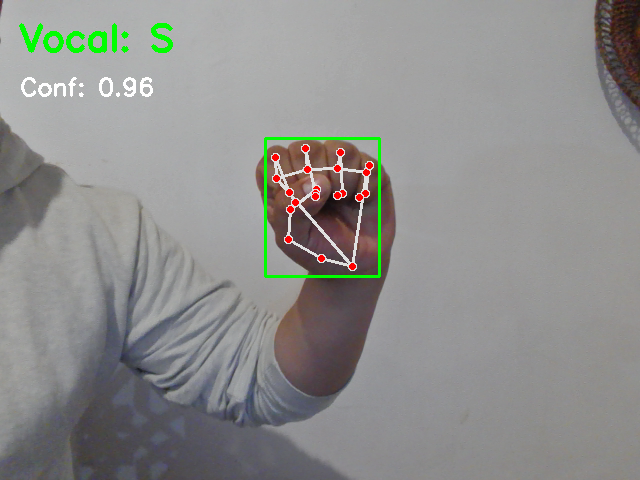
\includegraphics[width=\linewidth]{images/S1.png}
			\caption{Inferencia de la seña S en condiciones de buena iluminación.}
			\label{fig:inferencia_s_pc}
		\end{subfigure}
		\hfill
		\begin{subfigure}{0.48\textwidth}
			\centering
			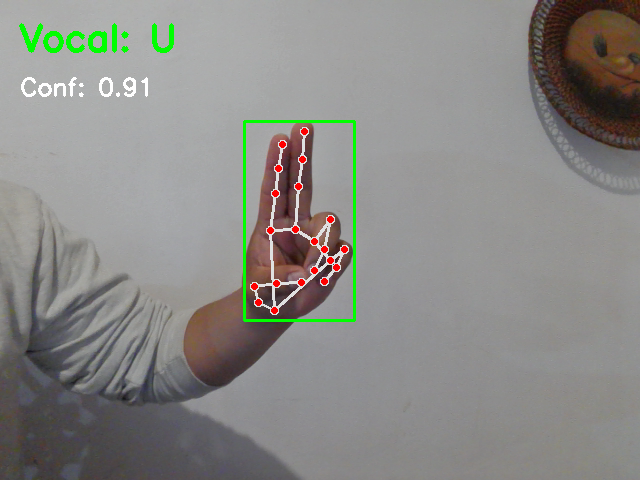
\includegraphics[width=\linewidth]{images/U1.png}
			\caption{Inferencia de la seña U en condiciones de buena iluminación.}
			\label{fig:inferencia_u_pc}
		\end{subfigure}
		\caption{Ejemplos de inferencia en entorno de escritorio bajo condiciones de iluminación favorables.}
		\label{fig:inferencia_pc_buena_luz}
	\end{figure}
	
	Las Figuras \ref{fig:inferencia_s_pc} y \ref{fig:inferencia_u_pc} muestran ejemplos visuales del comportamiento de la variante seleccionada en la inferencia en escritorio. En ambos casos se observa la detección correcta de los landmarks de la mano, el encuadre de la región detectada y la clasificación correspondiente con valores de confianza superiores a 0.90.
	
	
	\subsection{Selección de la arquitectura del modelo}
	
	En las primeras etapas del proyecto, desarrolladas principalmente en TT1, se exploraron distintos enfoques basados en CNN para el reconocimiento de señas estáticas de la LSM utilizando imágenes completas como entrada. Estas pruebas incluyeron diferentes arquitecturas orientadas al reconocimiento del alfabeto dactilológico a partir de fotografías capturadas mediante cámara, así como distintas configuraciones de entrenamiento y preprocesamiento de imágenes.
	
	Aunque las CNN lograban resultados favorables en entrenamiento, en las pruebas comenzaron a observarse problemas importantes de generalización al introducir variaciones de iluminación, cambios de fondo, diferencias en orientación de la mano y modificaciones en la distancia respecto a la cámara. En múltiples casos, el comportamiento del modelo dependía considerablemente de las condiciones visuales presentes en el entrenamiento, provocando disminuciones notables en estabilidad y consistencia en la inferencia continua.
	
	A partir de estas observaciones, se decidió replantear el enfoque general del modelo, sustituyendo el uso directo de imágenes por una representación estructurada basada en landmarks obtenidos mediante MediaPipe Hands. Este cambio permitió reducir significativamente la dependencia respecto al fondo y a las condiciones visuales del entorno, concentrando el proceso de clasificación principalmente en la geometría y posición relativa de la mano detectada.
	
	Con el nuevo enfoque basado en landmarks, se evaluaron distintas alternativas de clasificación compatibles con vectores de características de baja dimensionalidad, incluyendo algoritmos clásicos de aprendizaje automático y modelos neuronales ligeros orientados a ejecución móvil. Entre las alternativas consideradas se analizaron modelos como Support Vector Machine (SVM), Random Forest y perceptrones multicapa (MLP), priorizando criterios como estabilidad, capacidad de generalización, compatibilidad con TensorFlow Lite y facilidad de integración dentro del entorno Android utilizado en el proyecto.
	
	Tanto SVM como Random Forest mostraron resultados muy favorables en entorno de escritorio, alcanzando niveles de estabilidad y precisión comparables a los obtenidos posteriormente con la red neuronal. En particular, Random Forest presentó un comportamiento robusto en la inferencia continua utilizando landmarks extraídos con MediaPipe, mientras que SVM mostró una buena capacidad de separación entre clases incluso bajo ciertas variaciones de posición y orientación de la mano. Es por eso que inicialmente estos modelos fueron considerados como candidatos viables para la implementación final del prototipo.
	
	Pero conforme el proyecto avanzó hacia la integración móvil, comenzaron a identificarse limitaciones importantes relacionadas con la compatibilidad y despliegue de estos algoritmos dentro del entorno Android. A diferencia de las redes neuronales desarrolladas con TensorFlow, modelos como SVM y Random Forest no cuentan con una compatibilidad nativa directa con TensorFlow Lite, framework seleccionado para ejecutar inferencia local en dispositivos móviles.
	
	Aunque existen alternativas para implementar este tipo de modelos en Android, dichas soluciones implican procesos considerablemente más complejos, tales como la reimplementación manual de la lógica de inferencia, transpilar estructuras completas del modelo hacia código compatible con Android, utilizar bibliotecas externas no optimizadas para ejecución móvil o desarrollar mecanismos personalizados de clasificación fuera del flujo estándar de TensorFlow Lite. Estas alternativas incrementaban significativamente la complejidad del sistema, dificultaban el mantenimiento del proyecto y reducían parte de las ventajas de portabilidad y optimización que ofrece TensorFlow Lite para dispositivos móviles.
	
	El uso de TensorFlow Lite proporcionaba ventajas importantes relacionadas con optimización de memoria, aceleración mediante NNAPI(Es una API de Android diseñada específicamente para acelerar modelos de inteligencia artificial en dispositivos móviles) siempre y cuando el dispotivo fuera compatible, ademas de  compatibilidad con hardware móvil y facilidad de integración dentro del pipeline de inferencia desarrollado para Android. Debido a ello, mantener un flujo de trabajo completamente compatible con TensorFlow Lite se convirtió en un criterio prioritario en la selección final de la arquitectura del modelo.
	
	Por lo anterior se seleccionó un perceptrón multicapa (MLP) como arquitectura principal debido a su capacidad para modelar relaciones no lineales entre landmarks, su bajo costo computacional y su adecuada compatibilidad con inferencia móvil en dispositivos Android.
	
	
	\subsubsection{Arquitectura del perceptrón multicapa}
	
	El modelo de clasificación implementado en el presente trabajo corresponde a un perceptrón multicapa o MLP (\textit{Multilayer Perceptron}), seleccionado debido a que la entrada del sistema está conformada por un vector numérico de características y no por imágenes completas. En este enfoque, la información visual capturada por la cámara es transformada previamente mediante MediaPipe Hands en una representación geométrica compuesta por landmarks de la mano, reduciendo significativamente la dimensionalidad del problema y eliminando gran parte de la dependencia respecto al fondo y a las condiciones visuales del entorno.
	
	La entrada del modelo está conformada por un vector de 42 características, correspondiente a las coordenadas bidimensionales $(x,y)$ de los 21 landmarks detectados en la mano. 
	
	El uso de un vector de entrada de 42 características representa un equilibrio óptimo entre la fidelidad de la representación geométrica y el costo computacional del modelo. Desde la perspectiva de la \textit{maldición de la dimensionalidad}, una reducción en el número de características comprometería la topología de la mano, derivando en una pérdida de información crítica para distinguir señas morfológicamente similares. Por el contrario, un incremento innecesario en la dimensionalidad induciría redundancia estadística, elevando el riesgo de sobreajuste ($overfitting$) y penalizando la latencia de inferencia en dispositivos móviles con recursos limitados. Diversos trabajos especializados en el reconocimiento de gestos mediante \textit{landmarks} bidimensionales validan que esta representación compacta, procesada por modelos MLP y convertida a formatos de cuantización como TensorFlow Lite, ofrece una precisión robusta para sistemas embebidos en tiempo real \cite{Kumar2025GestureMLP, Goodfellow2016}.
	
	La arquitectura del clasificador se basa en el paradigma de redes densas completamente conectadas (\textit{Fully Connected Networks}), seleccionadas estratégicamente sobre otras arquitecturas como las CNN. Esta decisión se tomo debido a que la etapa de preprocesamiento mediante \textit{MediaPipe Hands} ya realiza una extracción de características cinemáticas, transformando datos de imagen crudos en un vector de características estructurado $\mathbf{x} \in \mathbb{R}^{42}$. Al operar sobre este espacio latente de baja dimensionalidad, el uso de convoluciones espaciales resulta redundante y computacionalmente ineficiente, permitiendo que un Perceptrón Multicapa (MLP) capture directamente las dependencias no lineales entre los \textit{landmarks} de la mano \cite{Goodfellow2016}.
	
	\paragraph{Fundamentación de Capas y Unidades Ocultas}
	La arquitectura fue diseñada bajo una lógica de \textbf{embudo de información} (\textit{Information Bottleneck}), estructurada de la siguiente manera:
	
	\begin{itemize}
		\item \textbf{Capa de Proyección (64 neuronas):} La primera capa oculta realiza una proyección del vector de entrada a un espacio de 64 dimensiones. Esta expansión de la dimensionalidad inicial es una técnica estándar para facilitar la \textit{separabilidad lineal} de las clases en problemas donde los datos de entrada están altamente correlacionados. Matemáticamente, permite que la red encuentre hiperplanos de decisión más complejos que los que podrían obtenerse directamente desde el espacio original de 42 dimensiones \cite{Geron2022HandsOnML}.
		
		\item \textbf{Capa de Abstracción y Síntesis (32 neuronas):} La segunda capa densa reduce la dimensionalidad interna. Este cuello de botella obliga a la red a descartar variaciones irrelevantes (ruido en la detección de puntos) y a retener únicamente los rasgos invariantes del gesto manual. Esta estructura jerárquica permite que las primeras capas aprendan relaciones geométricas básicas, mientras que las capas profundas sintetizan conceptos de alto nivel correspondientes a la configuración dactilar completa \cite{Chollet2021}.
	\end{itemize}
	
	\paragraph{Dinámica de Activación y Optimización del Gradiente}
	Se implementó la función de activación \textit{Rectified Linear Unit} (ReLU), definida como $f(z) = \max(0, z)$, en todas las capas ocultas. A diferencia de las funciones saturables como la sigmoide o $\tanh$, ReLU permite una propagación de gradientes más eficiente al evitar el fenómeno de \textit{Vanishing Gradient} en la región positiva. Desde la perspectiva de implementación en \textit{Android}, ReLU es computacionalmente económica, requiriendo únicamente una operación de umbralización a nivel de CPU/GPU, lo que garantiza una tasa de cuadros por segundo (FPS) estable en la inferencia continua \cite{Nair2010ReLU}.
	
	\paragraph{Estrategia de Regularización y Generalización}
	Para garantizar la robustez del modelo ante datos no vistos, se integró una capa de \textit{Dropout} con una probabilidad de desactivación $p=0.2$. Esta técnica actúa como una forma de entrenamiento de ensamble (\textit{Ensemble Learning}) al entrenar sub-redes aleatorias en cada iteración, lo que previene la co-adaptación de neuronas. La selección de una tasa del 20\% responde a un equilibrio crítico: una tasa mayor destruiría la capacidad representacional en una arquitectura ya compacta, mientras que una menor fallaría en mitigar el sobreajuste provocado por la alta densidad de los datos de entrenamiento \cite{Srivastava2014Dropout}.
	
	\paragraph{Capa de Clasificación y Convergencia Final}
	La capa de salida emplea una función \textit{Softmax} para normalizar las puntuaciones crudas (\textit{logits}) en una distribución de probabilidad multinominal donde $\sum P(y_i|x) = 1$. Esta interpretación probabilística es vital para el despliegue móvil, permitiendo establecer un umbral de confianza (\textit{threshold}) para descartar detecciones erróneas cuando la mano no realiza una seña válida. 
	
	Por último la arquitectura fue refinada para su integración en \textit{TensorFlow Lite}, asegurando que el grafo computacional resultante sea compatible con delegados de aceleración por hardware (GPU/NNAPI), logrando una latencia de inferencia optimizada para dispositivos con recursos limitados \cite{TensorFlowLite2024}.
	
	\subsubsection{Configuración del Entrenamiento y Protocolo de Validación}
	
	El proceso de entrenamiento se diseñó para garantizar la estabilidad del gradiente y la capacidad de generalización del modelo ante datos no observados. A continuación, se detallan los parámetros y criterios técnicos seleccionados:
	
	\paragraph{División del Conjunto de Datos y Estratificación}
	Para la evaluación del modelo, el dataset se dividió en tres subconjuntos independientes: entrenamiento (80\%), validación (10\%) y prueba (10\%). Se implementó una \textbf{división estratificada} (\textit{stratified split}), la cual asegura que la cantidad de ejemplos por cada clase de la LSM se mantenga proporcional en todos los grupos. Este procedimiento es fundamental para evitar que el modelo se sesgue; sin esto, el sistema podría aprender muy bien las señas que más se repiten en el dataset pero fallar con aquellas que tienen menos ejemplos, garantizando así que todas las letras se reconozcan con la misma precisión \cite{Geron2022HandsOnML}.
	
	\paragraph{Hiperparámetros del Proceso Estocástico}
	\begin{itemize}
		\item \textbf{Tamaño de Lote (Batch Size = 32):} Se seleccionó un tamaño de lote de 32 muestras para equilibrar la eficiencia del paralelismo en hardware y la calidad de la estimación del gradiente. Un lote pequeño introduce un "ruido" beneficioso que ayuda al optimizador a escapar de mínimos locales, mientras que mantiene un consumo de memoria volátil adecuado para las capacidades de la estación de trabajo \cite{Goodfellow2016}.
		\item \textbf{Épocas y Early Stopping:} El límite máximo se estableció en 100 épocas. No obstante, para prevenir el sobreajuste y optimizar el tiempo de cómputo, se integró un \textit{callback} de \textit{Early Stopping} con una paciencia de 10 épocas, monitoreando la pérdida en el conjunto de validación (\textit{val\_loss}). Este mecanismo detiene el proceso automáticamente cuando no se detectan mejoras significativas, restaurando los pesos del modelo al punto de menor error observado.
	\end{itemize}
	
	\paragraph{Función de Pérdida y Optimización}
	Se utilizó la función de pérdida \textbf{Sparse Categorical Crossentropy}. Al tratarse de un problema de clasificación multiclase donde las etiquetas están codificadas como enteros (0, 1, 2, ...), esta función permite calcular la entropía cruzada sin necesidad de transformar las etiquetas a vectores \textit{one-hot}, reduciendo el consumo de memoria en el entrenamiento.
	
	El proceso de optimización se llevó a cabo mediante el algoritmo \textbf{Adam} (\textit{Adaptive Moment Estimation}). Se seleccionó Adam debido a que combina las ventajas de los algoritmos AdaGrad y RMSProp, ajustando automáticamente la tasa de aprendizaje (\textit{learning rate}) para cada parámetro individualmente a través del cálculo de los momentos primero y segundo de los gradientes. Esto permite una convergencia más rápida y robusta en comparación con el descenso de gradiente estocástico (SGD) tradicional \cite{Kingma2014Adam}.
	
	\paragraph{Reproducibilidad y Control de Aleatoriedad}
	
	Debido a que procesos como la inicialización de pesos y la división del conjunto de datos incluyen componentes aleatorios, se establecieron semillas globales (\textit{seeds}) tanto en las librerías de Python (\texttt{NumPy}) como en \texttt{TensorFlow}. Esta práctica permite obtener resultados consistentes bajo las mismas condiciones de entrenamiento y facilita la repetición de los experimentos realizados en el desarrollo del prototipo \cite{TensorFlow2024}.
	
	\subsubsection{Flujo de Entrenamiento y Exportación}
	
	El proceso para obtener el clasificador final se dividió en etapas que garantizan la integridad de los datos y la portabilidad del modelo hacia dispositivos móviles.
	
	\paragraph{Preparación y Codificación de Etiquetas}
	Después de cargar el dataset desde el archivo \texttt{data.pickle}, se realizó una limpieza para asegurar que cada muestra contuviera exactamente 42 características, descartando registros incompletos. Posteriormente, se utilizó \textbf{LabelEncoder} para transformar las etiquetas de texto (letras de la LSM) en valores numéricos. Este paso es indispensable, ya que las redes neuronales solo pueden procesar tensores numéricos y no cadenas de texto de forma directa.
	
	\subsection{Evaluación y análisis de resultados}
	
	Cuando se concluyo el proceso de entrenamiento y exportación del modelo, se realizaron distintas pruebas experimentales con la intensión de evaluar el desempeño general del clasificador de señas y analizar el comportamiento de las diferentes estrategias implementadas en el desarrollo del proyecto.
	
	En esta etapa se compararon múltiples enfoques de clasificación, incluyendo modelos basados en CNN, algoritmos de aprendizaje automático clásico como Support Vector Machine (SVM) y Random Forest, así como el perceptrón multicapa (MLP) finalmente seleccionado para la implementación móvil. Estas pruebas permitieron identificar las ventajas y limitaciones de cada uno, particularmente en aspectos relacionados con la generalización, estabilidad de inferencia, compatibilidad con TensorFlow Lite y desempeño bajo condiciones reales de captura.
	
	Se analizaron diferentes estrategias de normalización y procesamiento de los \textit{landmarks} obtenidos mediante MediaPipe Hands, evaluando su impacto en la precisión del reconocimiento, estabilidad de las inferencias y robustez frente a variaciones de iluminación, orientación y ruido visual.
	
	A partir de este análisis fue posible justificar técnicamente la selección del modelo final implementado dentro de la aplicación en android .
	
	\subsubsection{Resultados del entrenamiento}
	
	Inicialmente se consideró que simplificar la información visual podría facilitar el aprendizaje del modelo, por lo que se implementaron pipelines basados en escala de grises, suavizado gaussiano y segmentación mediante umbral adaptativo.
	
	La hipótesis inicial consistía en que eliminar información cromática permitiría que la red neuronal se concentrara únicamente en la geometría de la mano y en la forma de las señas, disminuyendo así la dependencia respecto al color de piel, sombras, reflejos o condiciones variables de iluminación. Además, trabajar con imágenes segmentadas en escala de grises reducía considerablemente la complejidad visual y el tamaño efectivo de la información procesada por el modelo.
	
	También se observó que este enfoque no producía los resultados esperados en escenarios reales. Aunque las imágenes segmentadas parecían visualmente más limpias, la pérdida de información contextual y de detalles presentes en las imágenes RGB afectaba la capacidad de generalización de las CNN. En múltiples pruebas se detectó sensibilidad ante pequeños cambios de iluminación, pérdida parcial de contornos y dificultades para mantener estabilidad en inferencias continuas.
	
	Despues se realizaron entrenamientos utilizando imágenes RGB sin segmentación agresiva, conservando la información visual original de la escena. Estas imágenes fueron redimensionadas a una resolución de $224 \times 224$ píxeles mediante una estrategia de \textit{padding}, evitando deformaciones en la proporción de la mano. Se aplicaron técnicas de aumentación de datos en el entrenamiento, incluyendo variaciones de brillo, contraste, saturación, calidad JPEG y recortes aleatorios.
	
	Los resultados obtenidos demostraron que las arquitecturas de CNN alcanzaban un comportamiento considerablemente más estable utilizando imágenes RGB normalizadas a $224 \times 224$, particularmente en escenarios con variaciones moderadas de iluminación y fondos complejos. Por esta razón, las versiones finales de los modelos CNN fueron entrenadas utilizando imágenes RGB como entrada principal.
	
	\paragraph{Loss y comportamiento de convergencia}
	
	Se compararon las curvas de pérdida (\textit{loss}) obtenidas en el entrenamiento y validación de cada modelo. Estas curvas permiten observar la estabilidad del proceso de aprendizaje, la velocidad de convergencia y posibles indicios de sobreajuste.
	
	La función de pérdida (\textit{loss}) representa el error cometido por el modelo en el proceso de entrenamiento y permite medir qué tan alejadas se encuentran las predicciones generadas respecto a las clases reales del conjunto de datos. En términos generales, valores menores de pérdida indican un mejor ajuste del modelo en el aprendizaje \cite{goodfellow2016deep,geron2022hands}.
	
	En el entrenamiento se calcularon tanto la pérdida de entrenamiento (\textit{train loss}) como la pérdida de validación (\textit{validation loss}). La pérdida de entrenamiento corresponde al error obtenido utilizando las muestras empleadas directamente para ajustar los pesos de la red neuronal, mientras que la pérdida de validación se calcula utilizando datos que no participan en la actualización de parámetros y que permiten evaluar la capacidad de generalización del modelo \cite{goodfellow2016deep}.
	
	La comparación entre ambas curvas permite analizar distintos aspectos del comportamiento de aprendizaje de una red neuronal. Cuando ambas curvas disminuyen de forma progresiva y permanecen relativamente cercanas, el modelo suele presentar un proceso de convergencia estable. Por el contrario, diferencias crecientes entre entrenamiento y validación pueden indicar problemas de sobreajuste, donde el modelo memoriza características específicas del conjunto de entrenamiento y pierde capacidad de generalización frente a datos nuevos \cite{geron2022hands,chollet2021deep}.
	
	El sobreajuste (\textit{overfitting}) ocurre cuando un modelo aprende de manera excesiva características específicas presentes en el conjunto de entrenamiento, incluyendo patrones particulares, ruido o variaciones que no representan adecuadamente el comportamiento general de los datos. Como consecuencia, el modelo puede alcanzar métricas elevadas en el entrenamiento pero presentar un desempeño deficiente al enfrentarse a datos nuevos o escenarios reales \cite{goodfellow2016deep,chollet2021deep}.
	
	En términos prácticos, el sobreajuste suele identificarse cuando la pérdida de entrenamiento continúa disminuyendo mientras la pérdida de validación permanece estable o comienza a incrementarse progresivamente. Esto indica que el modelo mejora únicamente sobre los datos utilizados en el aprendizaje, perdiendo capacidad de generalización \cite{geron2022hands}.
	
	Por otra parte, el subajuste (\textit{underfitting}) ocurre cuando el modelo no logra aprender adecuadamente las características fundamentales del problema. En estos casos, tanto las métricas de entrenamiento como las de validación presentan resultados deficientes, reflejando que la arquitectura utilizada no posee suficiente capacidad de representación o que el proceso de entrenamiento resulta insuficiente \cite{goodfellow2016deep}.
	
	El análisis conjunto de las curvas de pérdida y precisión permite identificar este tipo de comportamientos en el entrenamiento de redes neuronales, facilitando la selección de arquitecturas y configuraciones más estables para tareas de clasificación.
	
	La Figura 44 muestra las curvas de pérdida correspondientes a las arquitecturas evaluadas en el entrenamiento.
	
	\begin{figure}[H]
		\centering
		
		\begin{subfigure}{0.48\textwidth}
			\centering
			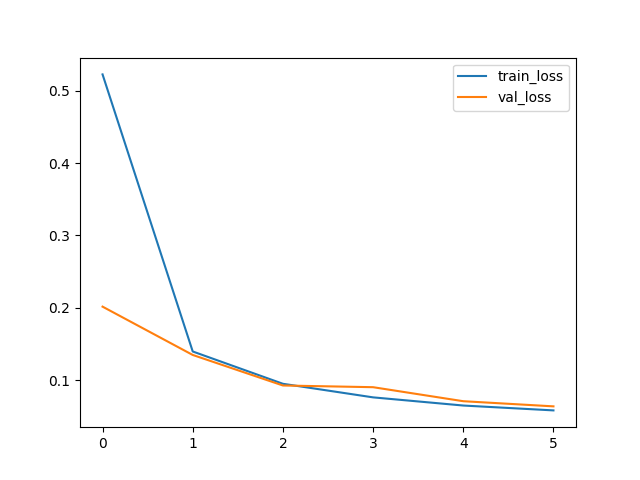
\includegraphics[width=\linewidth]{images/lc_rn50.png}
			\caption{Modelo A: ResNet50}
		\end{subfigure}
		\hfill
		\begin{subfigure}{0.48\textwidth}
			\centering
			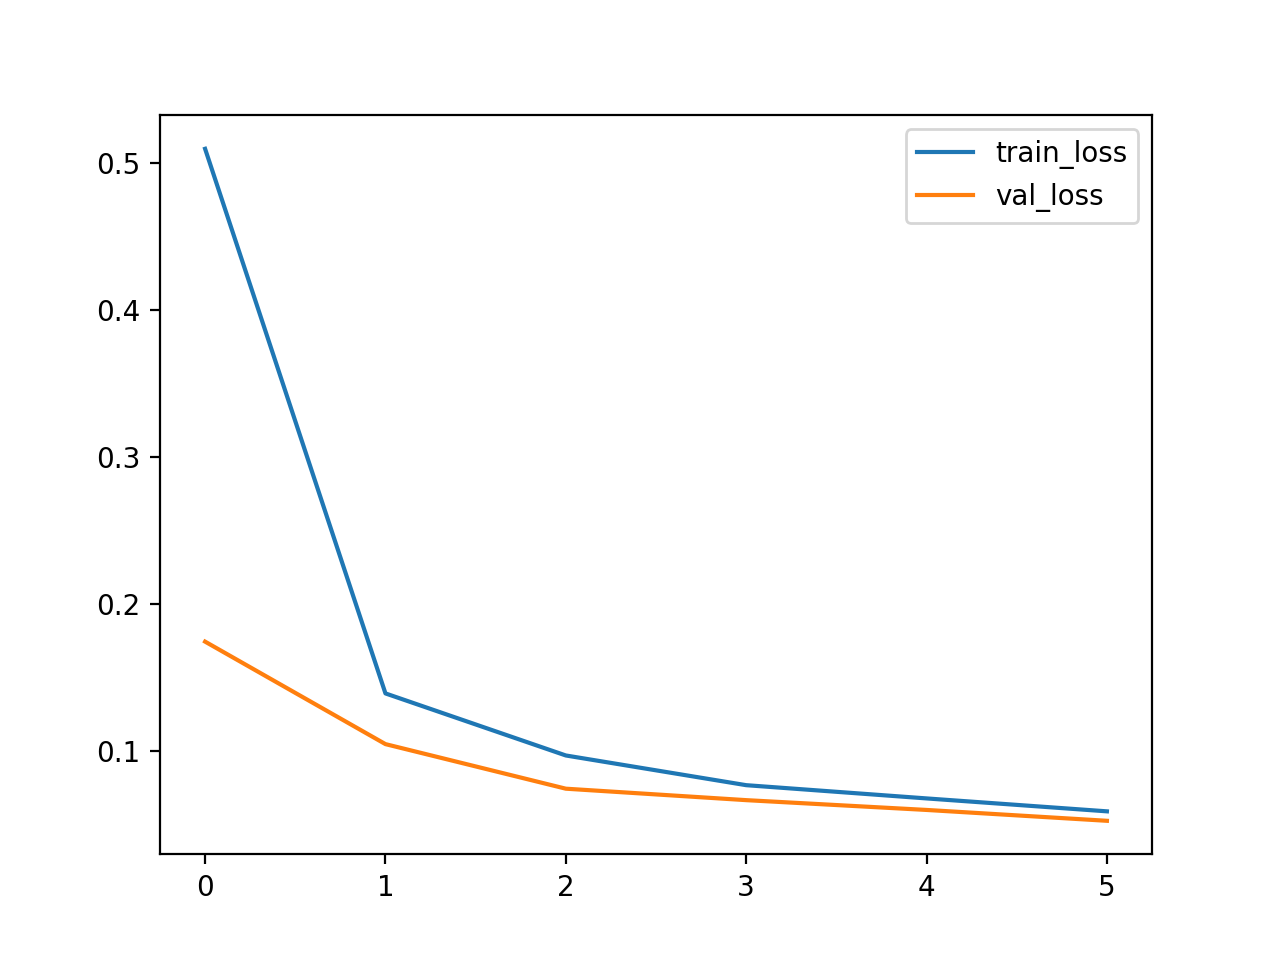
\includegraphics[width=\linewidth]{images/lc_mn2.png}
			\caption{Modelo B: MobileNetV2}
		\end{subfigure}
		
		\vspace{0.3cm}
		
		\begin{subfigure}{0.48\textwidth}
			\centering
			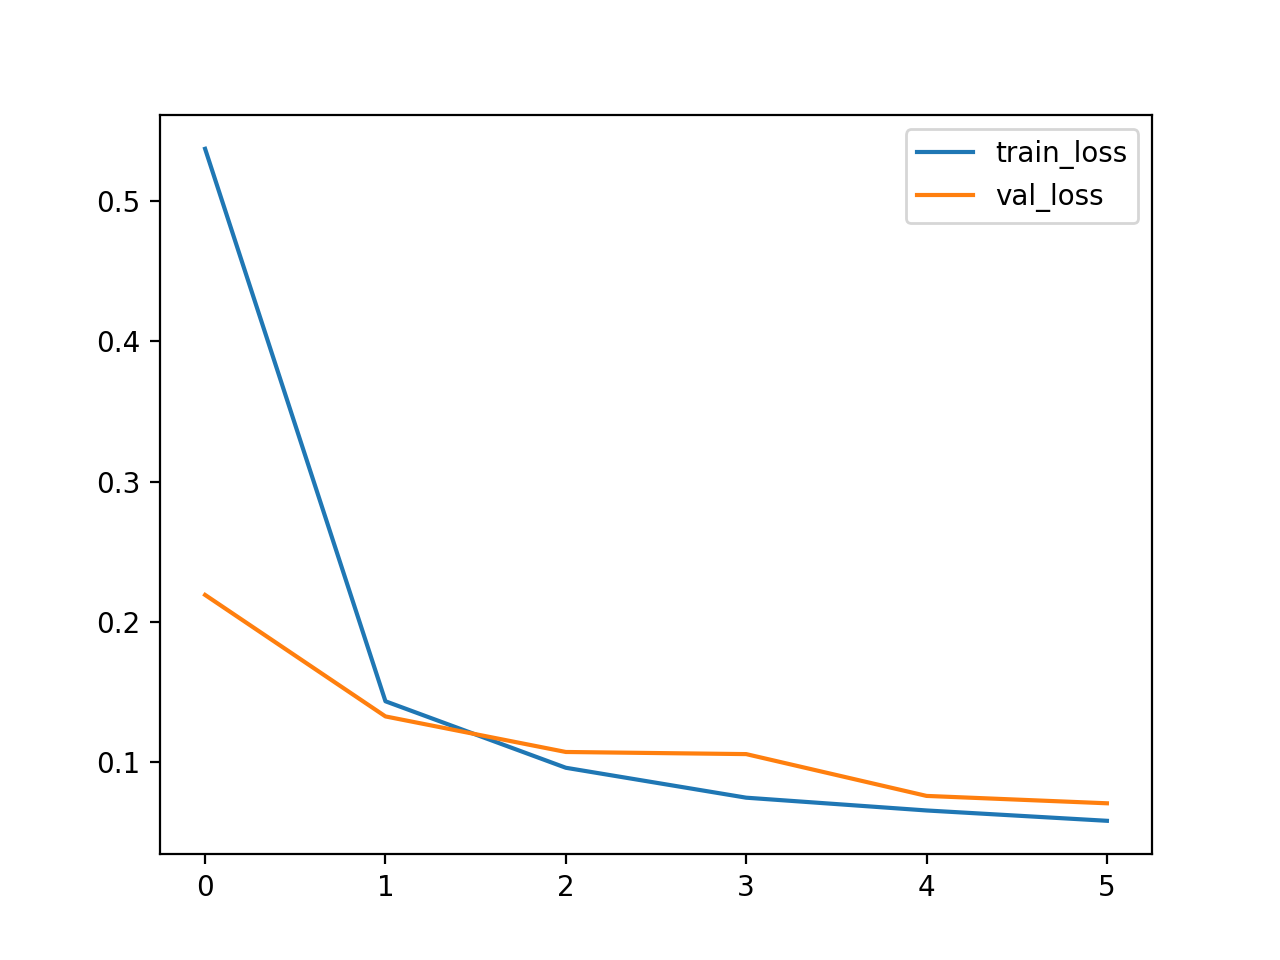
\includegraphics[width=\linewidth]{images/lc_mn3.png}
			\caption{Modelo C: MobileNetV3}
		\end{subfigure}
		\hfill
		\begin{subfigure}{0.48\textwidth}
			\centering
			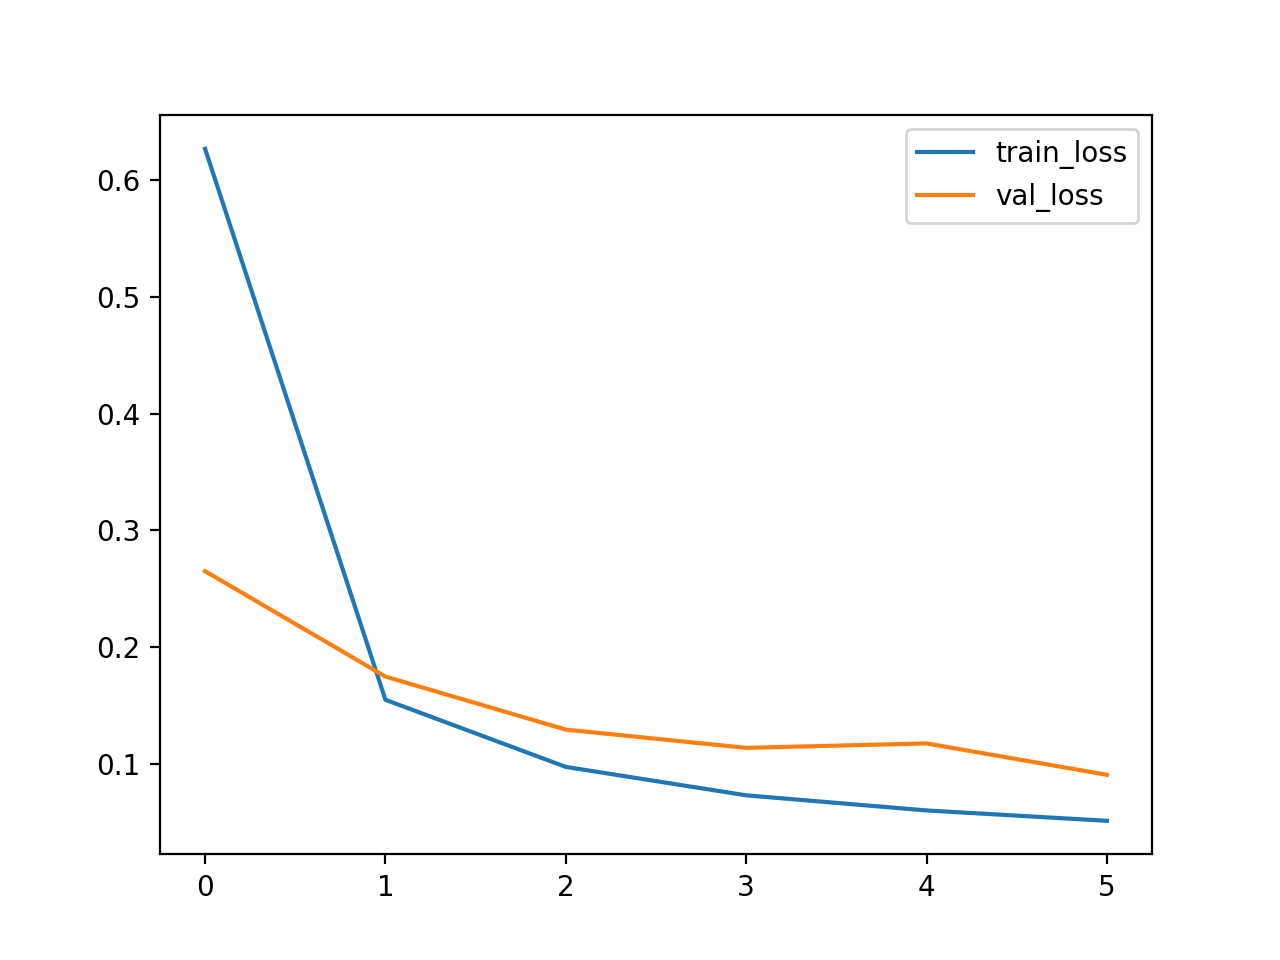
\includegraphics[width=\linewidth]{images/lc_enl.png}
			\caption{Modelo D: EfficientNet Lite0}
		\end{subfigure}
		
		\vspace{0.3cm}
		
		\begin{subfigure}{0.48\textwidth}
			\centering
			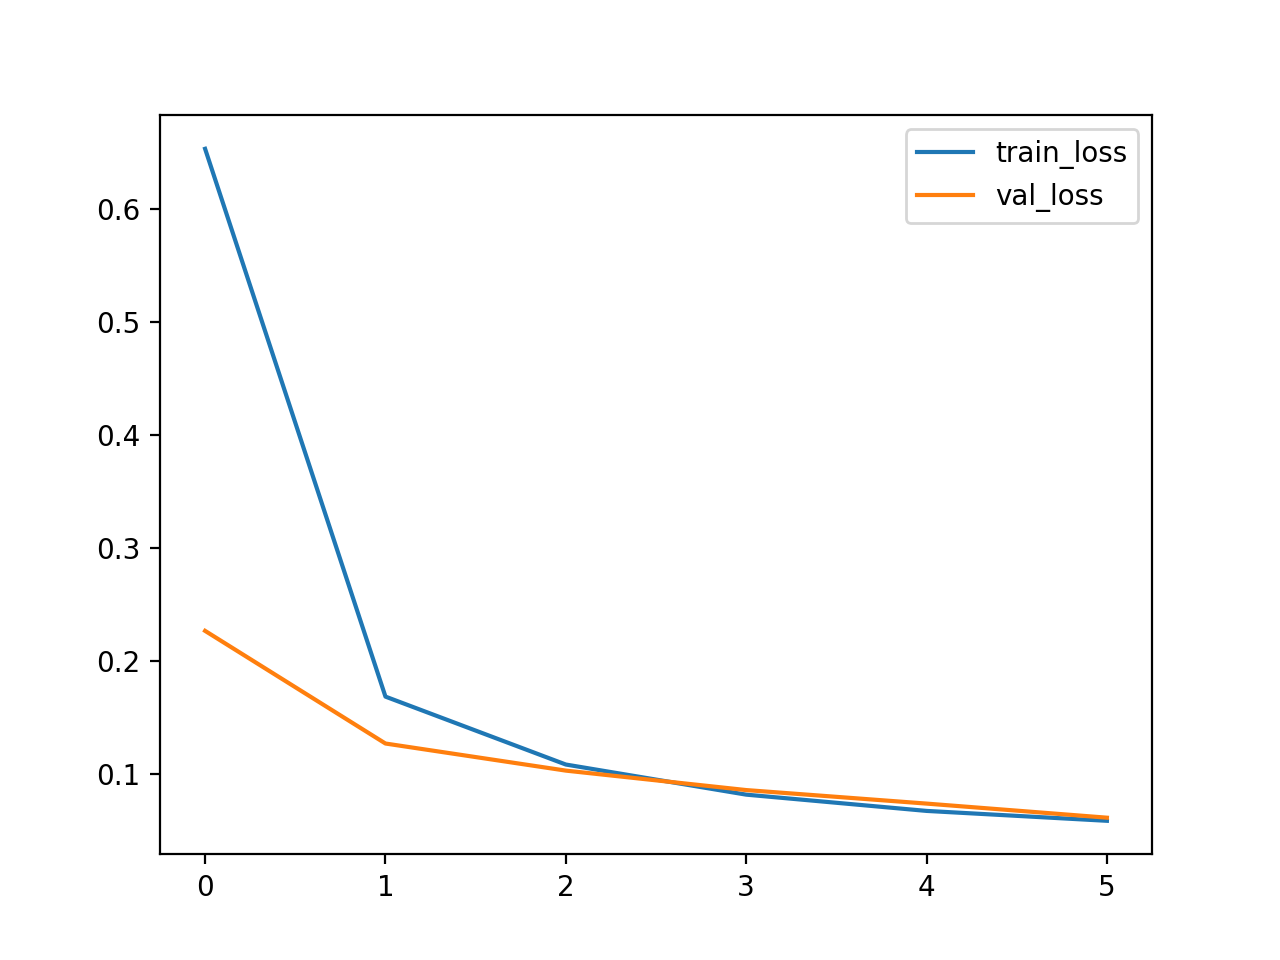
\includegraphics[width=\linewidth]{images/lc_en1.png}
			\caption{Modelo E: EfficientNet Lite1}
		\end{subfigure}
		
		\caption{Curvas de pérdida obtenidas en el entrenamiento y validación de las CNN evaluadas.}
		\label{fig:loss_modelos}
	\end{figure}
	
	El Modelo A (ResNet50) presentó una disminución rápida de la pérdida en las primeras épocas de entrenamiento, seguida de una estabilización progresiva tanto en entrenamiento como en validación. Las curvas permanecieron relativamente cercanas en todo el proceso, indicando un comportamiento estable y una capacidad de generalización adecuada dentro del conjunto de datos utilizado.
	
	En el caso del Modelo B (MobileNetV2), las curvas mostraron una convergencia progresiva y consistente. La separación reducida entre la pérdida de entrenamiento y validación sugiere que el modelo logró mantener estabilidad en el aprendizaje, sin presentar indicios severos de sobreajuste.
	
	El Modelo C (MobileNetV3) presentó un comportamiento similar al observado en MobileNetV2, mostrando una reducción importante de la pérdida en las primeras épocas y una estabilización gradual hacia las últimas iteraciones. Sin embargo, se observaron ligeras fluctuaciones en la curva de validación, indicando una estabilidad moderadamente menor respecto a otras arquitecturas evaluadas.
	
	El Modelo D (EfficientNet Lite0) mostró una reducción acelerada de la pérdida de entrenamiento; no obstante, la pérdida de validación presentó un comportamiento menos uniforme en las últimas épocas. Esta diferencia sugiere posibles dificultades de generalización y ligeros indicios de sobreajuste conforme avanzaba el entrenamiento.
	
	El Modelo E (EfficientNet Lite1) presentó una convergencia estable y progresiva tanto en entrenamiento como en validación. Las curvas permanecieron cercanas en prácticamente todo el proceso de aprendizaje, indicando un comportamiento relativamente estable y una adecuada capacidad de ajuste sobre el conjunto de datos utilizado.
	
	Se puede concluir que todas las arquitecturas evaluadas lograron converger adecuadamente en el entrenamiento, alcanzando valores reducidos de pérdida en las etapas finales. Sin embargo, aunque varias arquitecturas mostraron estabilidad dentro del entorno controlado del dataset, posteriormente se observaron limitaciones importantes de generalización en las pruebas de inferencia realizadas mediante cámara en escenarios reales.

	\paragraph{Curvas de entrenamiento}
	
	Además de la función de pérdida, otra métrica ampliamente utilizada en el entrenamiento de redes neuronales es la precisión (\textit{accuracy}). Esta métrica representa la proporción de muestras clasificadas correctamente respecto al total de ejemplos evaluados, permitiendo analizar el desempeño general del modelo en el proceso de aprendizaje \cite{goodfellow2016deep,geron2022hands}.
	
	En el proceso de entrenamiento se calcularon tanto la precisión de entrenamiento (\textit{train accuracy}) como la precisión de validación (\textit{validation accuracy}). La comparación entre ambas curvas permite observar la evolución del aprendizaje de la red neuronal a lo largo de las diferentes épocas de entrenamiento, así como analizar aspectos relacionados con estabilidad, velocidad de convergencia y capacidad de generalización \cite{chollet2021deep}.
	
	El eje horizontal de las gráficas representa las épocas (\textit{epochs}) de entrenamiento, donde cada época corresponde a una iteración completa sobre el conjunto de datos utilizado en el aprendizaje del modelo. Por otra parte, el eje vertical representa la precisión alcanzada por la arquitectura en cada etapa del entrenamiento.
	
	Las arquitecturas de CNN utilizadas en esta etapa fueron inicializadas utilizando pesos preentrenados obtenidos sobre el conjunto de datos ImageNet. Este enfoque de transferencia de aprendizaje (\textit{transfer learning}) permitió reutilizar características visuales previamente aprendidas por los modelos, acelerando considerablemente la convergencia en las primeras épocas de entrenamiento \cite{chollet2021deep,geron2022hands}.
	
	
	
	La Figura 45 muestra las curvas de precisión obtenidas en el entrenamiento y validación de las CNN evaluadas.
	
	\begin{figure}[H]
		\centering
		
		\begin{subfigure}{0.48\textwidth}
			\centering
			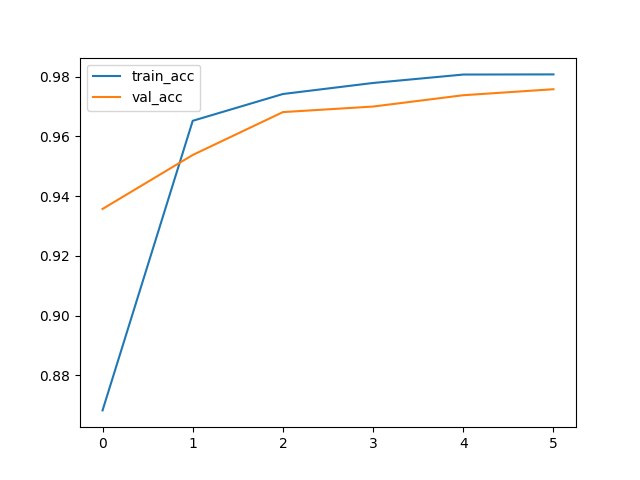
\includegraphics[width=\linewidth]{images/ac_rn50.png}
			\caption{Modelo A: ResNet50}
		\end{subfigure}
		\hfill
		\begin{subfigure}{0.48\textwidth}
			\centering
			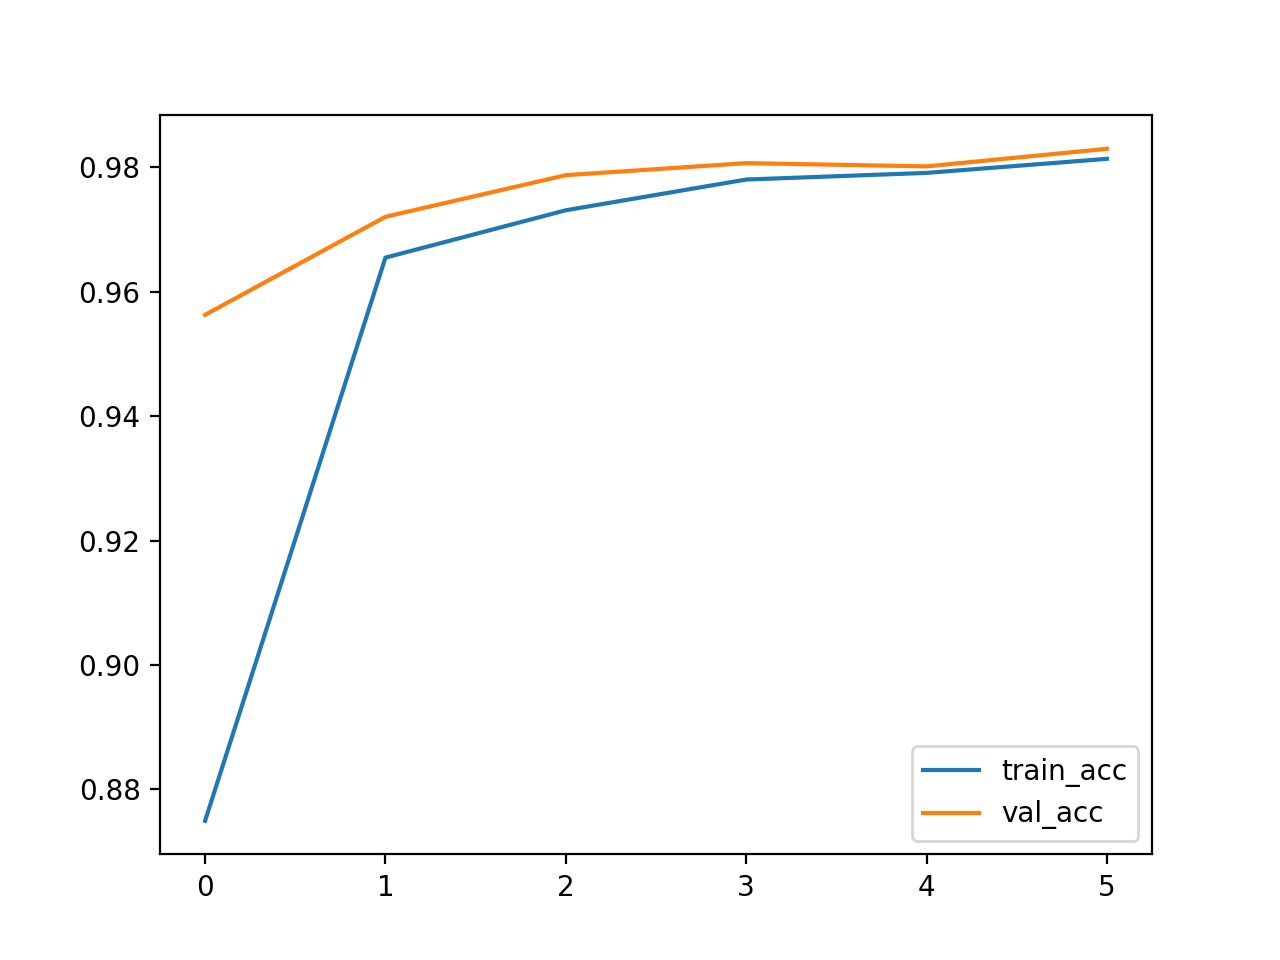
\includegraphics[width=\linewidth]{images/ac_mn2.png}
			\caption{Modelo B: MobileNetV2}
		\end{subfigure}
		
		\vspace{0.3cm}
		
		\begin{subfigure}{0.48\textwidth}
			\centering
			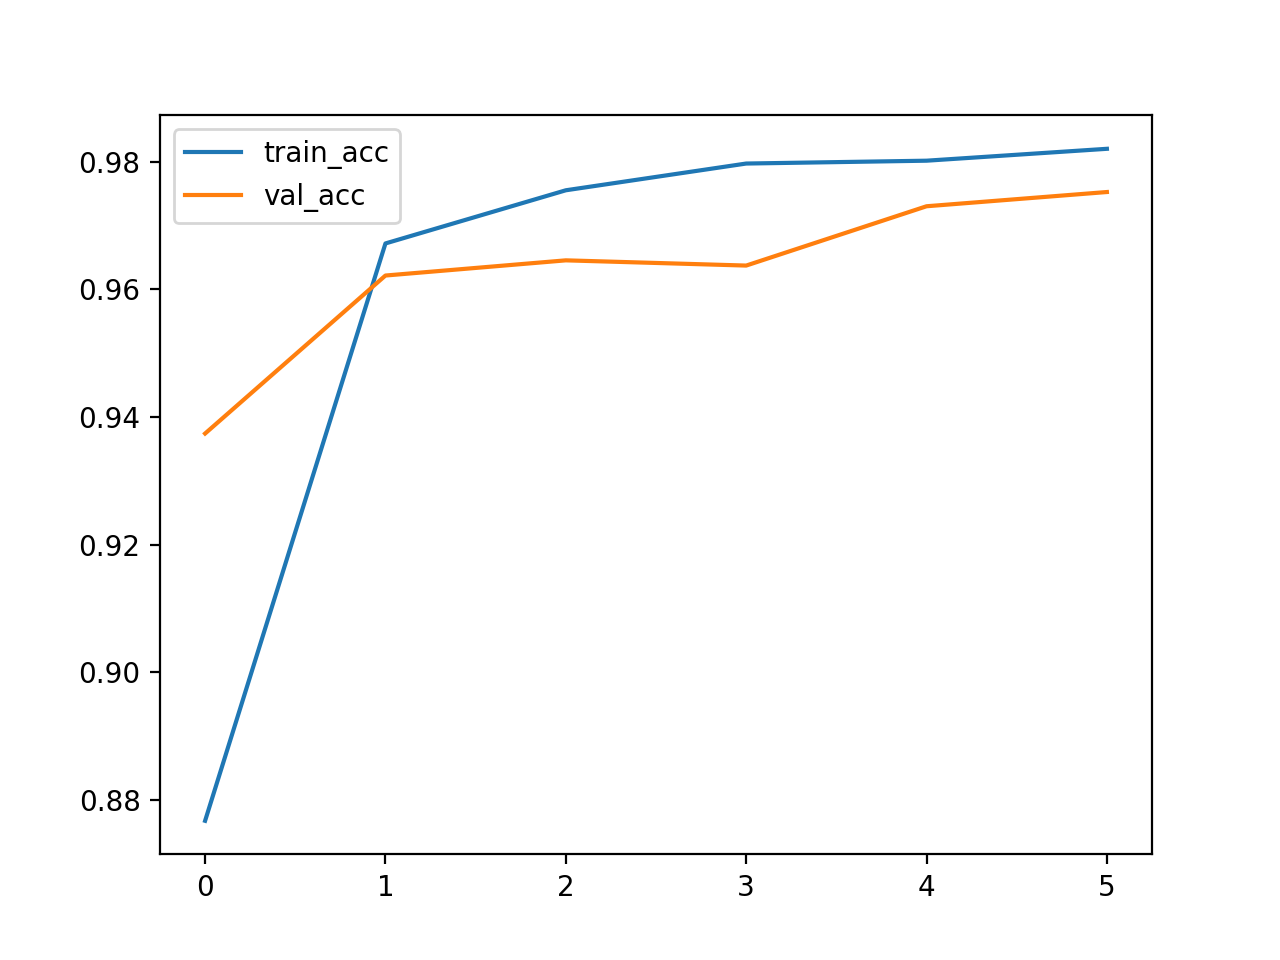
\includegraphics[width=\linewidth]{images/ac_mn3.png}
			\caption{Modelo C: MobileNetV3}
		\end{subfigure}
		\hfill
		\begin{subfigure}{0.48\textwidth}
			\centering
			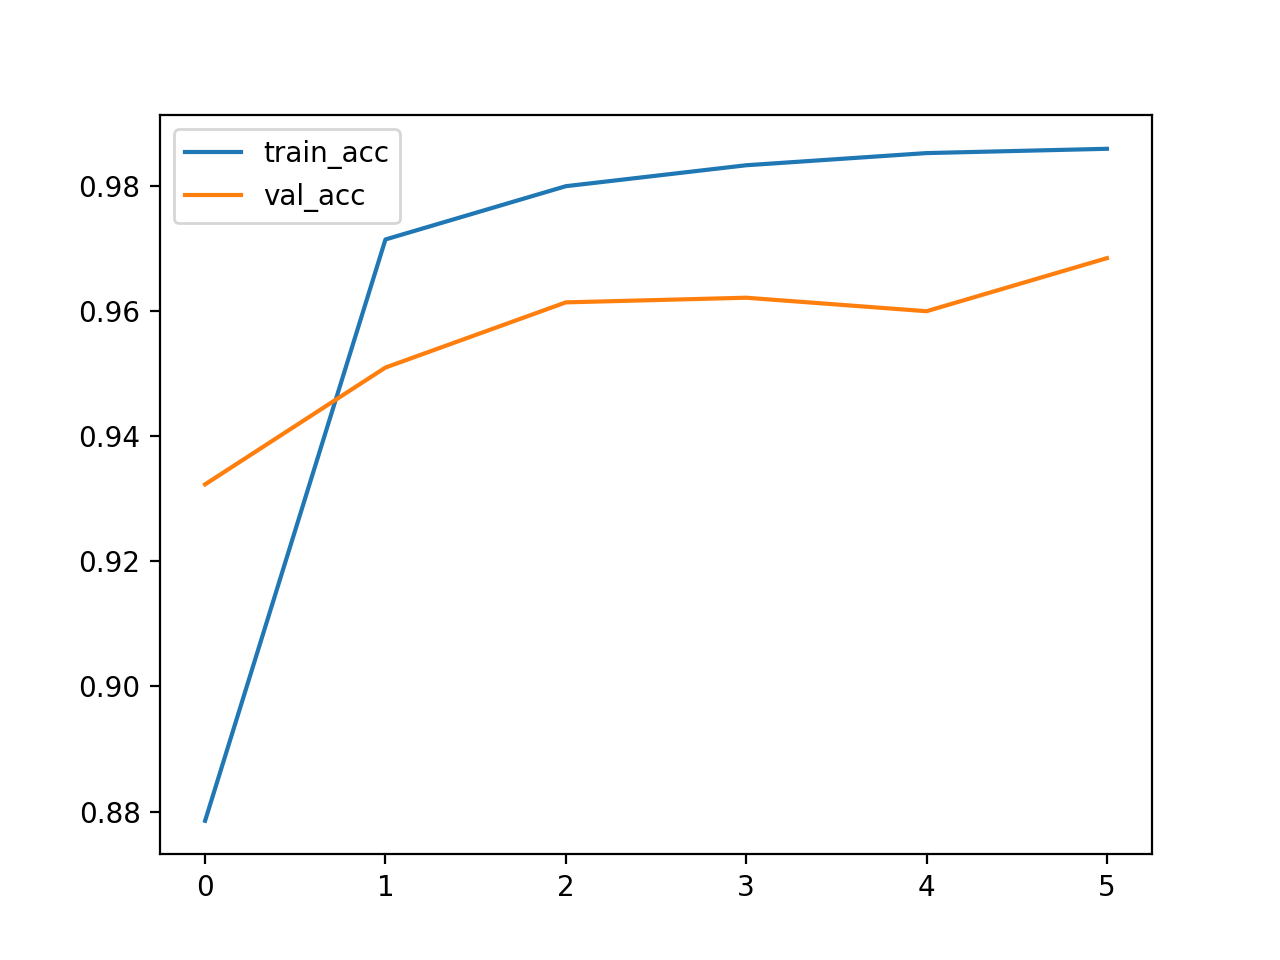
\includegraphics[width=\linewidth]{images/ac_en0.png}
			\caption{Modelo D: EfficientNet Lite0}
		\end{subfigure}
		
		\vspace{0.3cm}
		
		\begin{subfigure}{0.48\textwidth}
			\centering
			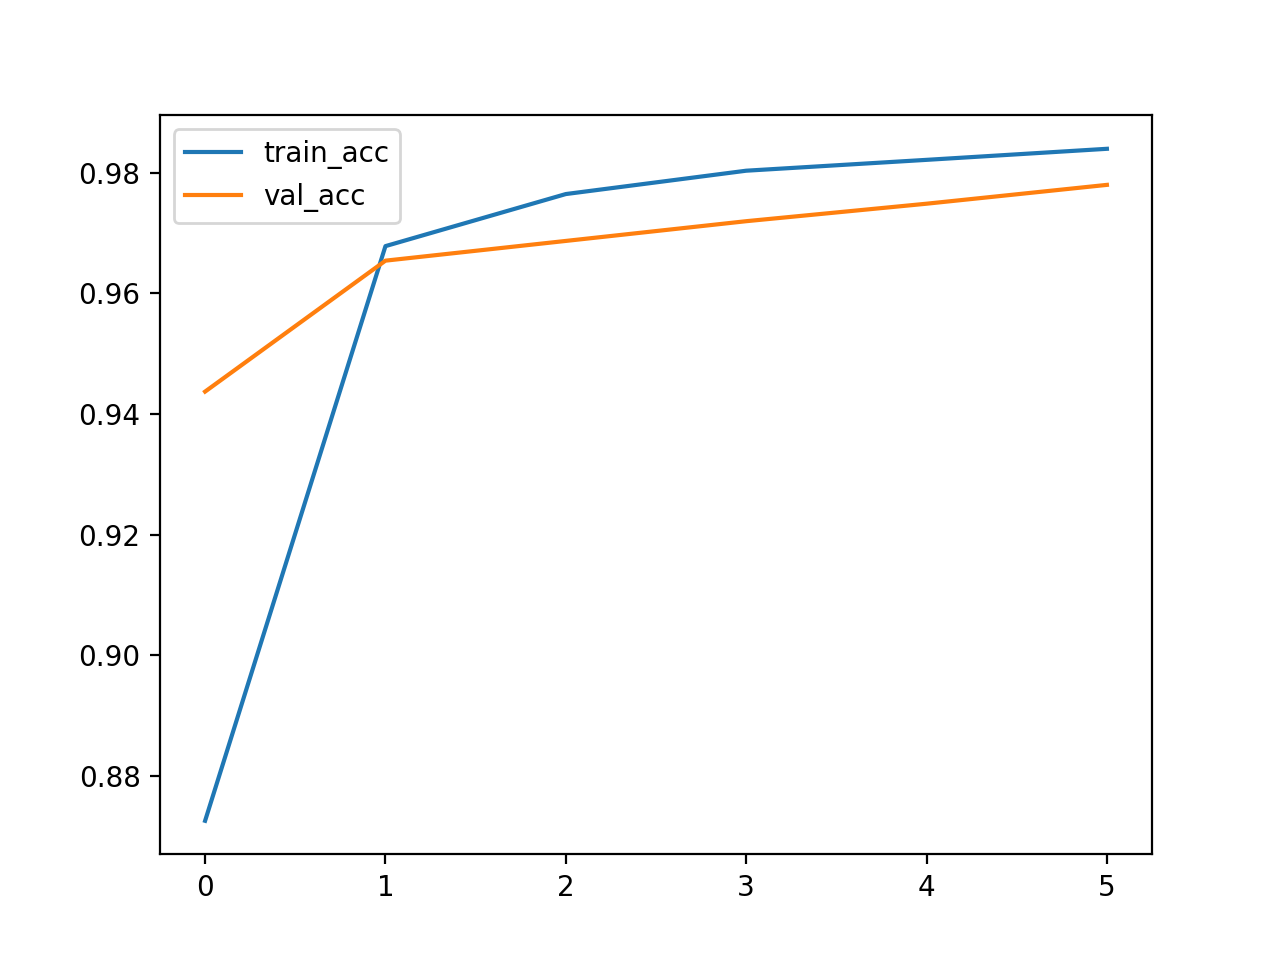
\includegraphics[width=\linewidth]{images/ac_en1.png}
			\caption{Modelo E: EfficientNet Lite1}
		\end{subfigure}
		
		\caption{Curvas de precisión obtenidas en el entrenamiento y validación de las CNN evaluadas.}
		\label{fig:acc_modelos}
	\end{figure}
	
	El Modelo A (ResNet50) presentó un incremento progresivo y estable de la precisión tanto en entrenamiento como en validación. Desde las primeras épocas se observó una convergencia rápida hacia valores elevados de precisión, manteniendo una diferencia reducida entre ambas curvas y evidenciando un comportamiento relativamente estable en el aprendizaje.
	
	En el caso del Modelo B (MobileNetV2), las curvas mostraron una convergencia acelerada en las primeras épocas de entrenamiento, alcanzando rápidamente valores superiores al 95\% de precisión. La proximidad entre las curvas de entrenamiento y validación indica un nivel moderado de generalización dentro del conjunto de datos utilizado.
	
	El Modelo C (MobileNetV3) presentó un comportamiento similar al observado en MobileNetV2, aunque la curva de validación mostró ligeras fluctuaciones en las últimas épocas. A pesar de ello, el modelo mantuvo valores elevados de precisión y una convergencia relativamente estable.
	
	El Modelo D (EfficientNet Lite0) alcanzó rápidamente valores altos de precisión de entrenamiento; sin embargo, la curva de validación mostró una separación ligeramente mayor respecto a la curva de entrenamiento conforme avanzaban las épocas. Este rendimiento puede interpretarse como un posible indicio de sobreajuste moderado.
	
	El Modelo E (EfficientNet Lite1) presentó una convergencia progresiva y estable, manteniendo una diferencia reducida entre entrenamiento y validación en prácticamente todo el proceso de aprendizaje. La estabilidad observada en ambas curvas sugiere una adecuada capacidad de ajuste sobre el conjunto de datos empleado.
	
	Todas las arquitecturas evaluadas alcanzaron valores elevados de precisión dentro del conjunto de validación, mostrando procesos de convergencia relativamente rápidos debido al uso de modelos preentrenados y técnicas de transferencia de aprendizaje. Sin embargo, aunque varias arquitecturas presentaron métricas elevadas durante entrenamiento y validación, posteriormente se observaron limitaciones importantes de generalización en las pruebas de inferencia realizadas mediante cámara en modo de inferencias continua.
	
	\subsubsection{Evaluación del modelo}
	
	Para analizar el desempeño de las arquitecturas evaluadas en el desarrollo del prototipo de reconocimiento de señas, se realizaron distintas pruebas experimentales utilizando métricas ampliamente empleadas en problemas de clasificación multiclase. Entre las principales métricas analizadas se incluyen precisión global (\textit{accuracy}), precisión por clase (\textit{precision}), exhaustividad (\textit{recall}) y puntuación F1 (\textit{F1-score}), las cuales permiten evaluar el comportamiento general de los modelos y su capacidad para clasificar correctamente las diferentes señas consideradas en el entrenamiento \cite{goodfellow2016deep,geron2022hands}.
	
	Además de las métricas obtenidas en validación y prueba, se realizaron experimentos adicionales de inferencia continua utilizando cámara de los dispositivos con el propósito de analizar la capacidad de generalización de las arquitecturas fuera de un entorno controlado. Estas pruebas permitieron identificar diferencias importantes entre el comportamiento observado en entrenamiento y el desempeño real obtenido bajo condiciones variables de captura, iluminación y orientación de la mano.
	
	
	\paragraph{Accuracy}\mbox{}\\
	
	La precisión global (\textit{accuracy}) representa la proporción de muestras clasificadas correctamente respecto al total de ejemplos evaluados. Esta métrica permite medir el desempeño general de un modelo de clasificación y es una de las medidas más utilizadas en procesos de entrenamiento y evaluación de redes neuronales \cite{goodfellow2016deep,geron2022hands}.
	
	Formalmente, la precisión global puede expresarse mediante la Ecuación \ref{eq:accuracy}.
	
	\begin{equation}
		\label{eq:accuracy}
		Accuracy = \frac{TP + TN}{TP + TN + FP + FN}
	\end{equation}
	
	donde:
	\begin{itemize}
		\item $TP$ corresponde a verdaderos positivos (\textit{True Positives}),
		\item $TN$ corresponde a verdaderos negativos (\textit{True Negatives}),
		\item $FP$ corresponde a falsos positivos (\textit{False Positives}),
		\item $FN$ corresponde a falsos negativos (\textit{False Negatives}).
	\end{itemize}
	
	En problemas de clasificación multiclase, esta métrica permite estimar el porcentaje total de predicciones correctas realizadas por el modelo sobre el conjunto de prueba. Valores cercanos a 1 indican un mejor desempeño general de clasificación \cite{chollet2021deep}.
	
	
	
	
	\paragraph{ACC de CNN}\mbox{}\\
	{
		\rowcolors{2}{rowblue}{white}
		
		\small
		\renewcommand{\arraystretch}{1.15}
		
		\begin{table}[H]
			\centering
			\caption{Comparación de precisión global (\textit{accuracy}) obtenida por las CNN.}
			\label{tab:cnn_accuracy}
			
			\begin{tabular}{
					!{\vrule width 0.6pt}
					>{\centering\arraybackslash}p{4.2cm}
					!{\vrule width 0.6pt}
					>{\centering\arraybackslash}p{3.2cm}
					!{\vrule width 0.6pt}
					>{\centering\arraybackslash}p{3.6cm}
					!{\vrule width 0.6pt}
				}
				\hline
				\rowcolor{headerblue}
				\textcolor{white}{\textbf{Modelo}} &
				\textcolor{white}{\textbf{Test Accuracy}} &
				\textcolor{white}{\textbf{Validation Accuracy}} \\
				\hline
				
				ResNet50 & 97.80\% & 97.58\% \\
				\hline
				MobileNetV2 & 97.91\% & 98.29\% \\
				\hline
				MobileNetV3 Large & 97.62\% & 97.52\% \\
				\hline
				EfficientNet Lite0 & 96.80\% & 96.84\% \\
				\hline
				EfficientNet Lite1 & 97.82\% & 97.79\% \\
				\hline
				
			\end{tabular}
		\end{table}
	}
		
	\paragraph{ACC de land marks}\mbox{}\\
	
	\rowcolors{2}{rowblue}{white}
	
	\small
	\renewcommand{\arraystretch}{1.15}
	
	\begin{table}[H]
		\centering
		\caption{Comparación de precisión global (\textit{accuracy}) obtenida por los modelos evaluados utilizando landmarks extraídos mediante MediaPipe Hands.}
		\label{tab:landmarks_accuracy}
		
		\begin{tabular}{|p{4.2cm}|p{3.5cm}|}
			\hline
			\rowcolor{headerblue}
			\headercell{Modelo} &
			\headercell{Test Accuracy} \\
			\hline
			
			MLP Landmarks &
			98.79\% \\
			\hline
			
			Random Forest Landmarks &
			98.26\% \\
			\hline
			
			SVM Landmarks &
			99.06\% \\
			\hline
			
		\end{tabular}
	\end{table}
	
	
	En estos resultados tanto las CNN como los modelos basados en landmarks alcanzaron valores elevados de precisión  durante las pruebas realizadas sobre los conjuntos de evaluación. En el caso de las CNN, las arquitecturas evaluadas lograron precisiones superiores al 96\%, destacando MobileNetV2 y EfficientNet Lite1 como los modelos con mejor desempeño dentro de este grupo.
	
	Los modelos entrenados utilizando landmarks extraídos mediante MediaPipe Hands alcanzaron resultados ligeramente superiores, particularmente el modelo SVM Landmarks, el cual obtuvo una precisión global de 99.06\%. Estos resultados sugieren que las representaciones geométricas basadas en landmarks podrían permiten reducir variaciones relacionadas con iluminación, fondo y condiciones de captura, favoreciendo una mayor capacidad de generalización respecto a los enfoques basados directamente en imágenes RGB.
	
	\paragraph{Precision}\mbox{}\\

	La precisión (\textit{precision}) es una métrica utilizada para evaluar la proporción de predicciones positivas realizadas correctamente por un modelo de clasificación. Esta métrica permite medir qué tan confiables son las clases predichas por la arquitectura, particularmente en problemas donde resulta importante minimizar falsas clasificaciones positivas \cite{goodfellow2016deep,geron2022hands}.
	
	Formalmente, la precisión puede expresarse mediante la Ecuación \ref{eq:precision}.
	
	\begin{equation}
		\label{eq:precision}
		Precision = \frac{TP}{TP + FP}
	\end{equation}
	
	donde:
	\begin{itemize}
		\item $TP$ corresponde a verdaderos positivos (\textit{True Positives}),
		\item $FP$ corresponde a falsos positivos (\textit{False Positives}).
	\end{itemize}
	
	En problemas de clasificación multiclase, la precisión permite analizar qué tan frecuentemente las muestras clasificadas dentro de una determinada categoría corresponden realmente a dicha clase. Valores elevados de precisión indican una menor cantidad de falsas clasificaciones positivas \cite{chollet2021deep}.
	
	A continuación, se presentan los resultados de precisión obtenidos por las CNN y por los modelos basados en landmarks evaluados en el desarrollo del prototipo.
	
	\paragraph{CNN}\mbox{}\\
	{
		\rowcolors{2}{rowblue}{white}
		
		\small
		\renewcommand{\arraystretch}{1.15}
		
		\begin{table}[H]
			\centering
			\caption{Comparación de precisión (\textit{precision}) obtenida por las CNN.}
			\label{tab:cnn_precision}
			
			\begin{tabular}{
					!{\vrule width 0.6pt}
					>{\centering\arraybackslash}p{4.2cm}
					!{\vrule width 0.6pt}
					>{\centering\arraybackslash}p{4.0cm}
					!{\vrule width 0.6pt}
				}
				\hline
				
				\rowcolor{headerblue}
				\textcolor{white}{\textbf{Modelo}} &
				\textcolor{white}{\textbf{Precision}} \\
				
				\hline
				
				ResNet50 & 97.80\% \\
				\hline
				
				MobileNetV2 & 97.84\% \\
				\hline
				
				MobileNetV3 Large & 97.62\% \\
				\hline
				
				EfficientNet Lite0 & 96.83\% \\
				\hline
				
				EfficientNet Lite1 & 97.78\% \\
				\hline
				
			\end{tabular}
		\end{table}
	}
	
	\paragraph{Landmarks}\mbox{}\\
	
	{
		\rowcolors{2}{rowblue}{white}
		
		\small
		\renewcommand{\arraystretch}{1.15}
		
		\begin{table}[H]
			\centering
			\caption{Comparación de precisión (\textit{precision}) obtenida por los modelos evaluados utilizando landmarks extraídos mediante MediaPipe Hands.}
			\label{tab:landmarks_precision}
			
			\begin{tabular}{
					!{\vrule width 0.6pt}
					>{\centering\arraybackslash}p{5.5cm}
					!{\vrule width 0.6pt}
					>{\centering\arraybackslash}p{4.0cm}
					!{\vrule width 0.6pt}
				}
				\hline
				
				\rowcolor{headerblue}
				\textcolor{white}{\textbf{Modelo}} &
				\textcolor{white}{\textbf{Precision}} \\
				
				\hline
				
				MLP Landmarks &
				98.76\% \\
				\hline
				
				Random Forest Landmarks &
				98.25\% \\
				\hline
				
				SVM Landmarks &
				99.03\% \\
				\hline
				
			\end{tabular}
		\end{table}
	}
	
	
	\paragraph{Recall}\mbox{}\\
	
	La exhaustividad (\textit{recall}) es una métrica utilizada para medir la capacidad de un modelo de clasificación para identificar correctamente las muestras pertenecientes a una determinada clase. Esta métrica permite evaluar qué proporción de los ejemplos positivos reales fue clasificada correctamente por el modelo \cite{goodfellow2016deep,geron2022hands}.
	
	Formalmente, la exhaustividad puede expresarse mediante la Ecuación \ref{eq:recall}.
	
	\begin{equation}
		\label{eq:recall}
		Recall = \frac{TP}{TP + FN}
	\end{equation}
	
	donde:
	\begin{itemize}
		\item $TP$ corresponde a verdaderos positivos (\textit{True Positives}),
		\item $FN$ corresponde a falsos negativos (\textit{False Negatives}).
	\end{itemize}
	
	En problemas de clasificación multiclase, esta métrica permite analizar la capacidad del modelo para reconocer correctamente las diferentes categorías evaluadas, reduciendo la cantidad de muestras positivas clasificadas erróneamente como pertenecientes a otra clase \cite{chollet2021deep}.
	
	A continuación, se presentan los resultados de exhaustividad obtenidos por las CNN y los modelos basados en landmarks evaluados en el desarrollo  del clasificador de señas.
	
	\paragraph{CNN}\mbox{}\\
	{
		\rowcolors{2}{rowblue}{white}
		
		\small
		\renewcommand{\arraystretch}{1.15}
		
		\begin{table}[H]
			\centering
			\caption{Comparación de exhaustividad (\textit{recall}) obtenida por las CNN.}
			\label{tab:cnn_recall}
			
			\begin{tabular}{
					!{\vrule width 0.6pt}
					>{\centering\arraybackslash}p{4.2cm}
					!{\vrule width 0.6pt}
					>{\centering\arraybackslash}p{4.0cm}
					!{\vrule width 0.6pt}
				}
				\hline
				
				\rowcolor{headerblue}
				\textcolor{white}{\textbf{Modelo}} &
				\textcolor{white}{\textbf{Recall}} \\
				
				\hline
				
				ResNet50 &
				97.80\% \\
				\hline
				
				MobileNetV2 &
				97.92\% \\
				\hline
				
				MobileNetV3 Large &
				97.62\% \\
				\hline
				
				EfficientNet Lite0 &
				96.80\% \\
				\hline
				
				EfficientNet Lite1 &
				97.82\% \\
				\hline
				
			\end{tabular}
		\end{table}
	}
	
	
	\paragraph{Landmarks}\mbox{}\\
	
	{
		\rowcolors{2}{rowblue}{white}
		
		\small
		\renewcommand{\arraystretch}{1.15}
		
		\begin{table}[H]
			\centering
			\caption{Comparación de exhaustividad (\textit{recall}) obtenida por los modelos evaluados utilizando landmarks extraídos mediante MediaPipe Hands.}
			\label{tab:landmarks_recall}
			
			\begin{tabular}{
					!{\vrule width 0.6pt}
					>{\centering\arraybackslash}p{5.5cm}
					!{\vrule width 0.6pt}
					>{\centering\arraybackslash}p{4.0cm}
					!{\vrule width 0.6pt}
				}
				\hline
				
				\rowcolor{headerblue}
				\textcolor{white}{\textbf{Modelo}} &
				\textcolor{white}{\textbf{Recall}} \\
				
				\hline
				
				MLP Landmarks &
				98.74\% \\
				\hline
				
				Random Forest Landmarks &
				98.24\% \\
				\hline
				
				SVM Landmarks &
				99.02\% \\
				\hline
				
			\end{tabular}
		\end{table}
	}
	
	\paragraph{F1-score}\mbox{}\\
	
	La puntuación F1 (\textit{F1-score}) es una métrica utilizada para combinar en un único valor el comportamiento de precisión (\textit{precision}) y exhaustividad (\textit{recall}) de un modelo de clasificación. Esta métrica es útil en problemas multiclase, ya que permite evaluar de forma equilibrada tanto la capacidad del modelo para realizar predicciones correctas como su habilidad para identificar adecuadamente las diferentes clases presentes en el conjunto de datos \cite{goodfellow2016deep,geron2022hands}.
	
	Formalmente, la puntuación F1 puede expresarse mediante la Ecuación \ref{eq:f1score}.
	
	\begin{equation}
		\label{eq:f1score}
		F1 = 2 \cdot \frac{Precision \cdot Recall}{Precision + Recall}
	\end{equation}
	
	donde:
	\begin{itemize}
		\item $Precision$ corresponde a la precisión del modelo,
		\item $Recall$ corresponde a la exhaustividad del modelo.
	\end{itemize}
	
	La puntuación F1 toma valores entre 0 y 1, donde valores cercanos a 1 indican un mejor equilibrio entre precisión y exhaustividad. Debido a ello, esta métrica es ampliamente utilizada para evaluar modelos de clasificación en tareas de reconocimiento de patrones y visión computacional \cite{chollet2021deep}.
	
	A continuación, se presentan los resultados de puntuación F1 obtenidos por las CNN y los modelos basados en landmarks evaluados.
	\paragraph{CNN}\mbox{}\\
	
	{
		\rowcolors{2}{rowblue}{white}
		
		\small
		\renewcommand{\arraystretch}{1.15}
		
		\begin{table}[H]
			\centering
			\caption{Comparación de puntuación F1 (\textit{F1-score}) obtenida por los modelos evaluados utilizando landmarks extraídos mediante MediaPipe Hands.}
			\label{tab:landmarks_f1}
			
			\begin{tabular}{
					!{\vrule width 0.6pt}
					>{\centering\arraybackslash}p{5.5cm}
					!{\vrule width 0.6pt}
					>{\centering\arraybackslash}p{4.0cm}
					!{\vrule width 0.6pt}
				}
				\hline
				
				\rowcolor{headerblue}
				\textcolor{white}{\textbf{Modelo}} &
				\textcolor{white}{\textbf{F1-score}} \\
				
				\hline
				
				MLP Landmarks &
				98.73\% \\
				\hline
				
				Random Forest Landmarks &
				98.23\% \\
				\hline
				
				SVM Landmarks &
				99.01\% \\
				\hline
				
			\end{tabular}
		\end{table}
	}
	
	
	\paragraph{Landmarks}\mbox{}\\
	
	{
		\rowcolors{2}{rowblue}{white}
		
		\small
		\renewcommand{\arraystretch}{1.15}
		
		\begin{table}[H]
			\centering
			\caption{Comparación de puntuación F1 (\textit{F1-score}) obtenida por las CNN.}
			\label{tab:cnn_f1}
			
			\begin{tabular}{
					!{\vrule width 0.6pt}
					>{\centering\arraybackslash}p{4.2cm}
					!{\vrule width 0.6pt}
					>{\centering\arraybackslash}p{4.0cm}
					!{\vrule width 0.6pt}
				}
				\hline
				
				\rowcolor{headerblue}
				\textcolor{white}{\textbf{Modelo}} &
				\textcolor{white}{\textbf{F1-score}} \\
				
				\hline
				
				ResNet50 &
				97.80\% \\
				\hline
				
				MobileNetV2 &
				97.84\% \\
				\hline
				
				MobileNetV3 Large &
				97.62\% \\
				\hline
				
				EfficientNet Lite0 &
				96.83\% \\
				\hline
				
				EfficientNet Lite1 &
				97.78\% \\
				\hline
				
			\end{tabular}
		\end{table}
	}
	
	
	El análisis conjunto de las métricas de exactitud (\textit{accuracy}), precisión (\textit{precision}), exhaustividad (\textit{recall}) y puntuación F1 (\textit{F1-score}) permitió evaluar de manera más completa el comportamiento de las diferentes arquitecturas utilizadas en el desarrollo del prototipo de reconocimiento de señas.
	
	En el caso de las CNN basadas directamente en imágenes RGB, los resultados obtenidos mostraron valores elevados en todas las métricas evaluadas, alcanzando desempeños superiores al 96\% en la mayoría de los casos. Particularmente, MobileNetV2 y EfficientNet Lite1 presentaron los mejores resultados globales dentro de este grupo, mostrando un comportamiento relativamente estable sobre el conjunto de prueba \cite{goodfellow2016deep}. Las diferencias reducidas entre precisión, exhaustividad y puntuación F1 indican que las arquitecturas lograron mantener un comportamiento equilibrado entre falsas clasificaciones positivas y negativas.
	
	Aunque las métricas obtenidas en evaluación controlada resultaron considerablemente altas, posteriormente se observaron limitaciones importantes en las pruebas de inferencia realizadas mediante cámara en escenarios reales. Estas diferencias evidenciaron que un desempeño elevado sobre conjuntos de prueba no garantizaba necesariamente una capacidad robusta de generalización bajo condiciones variables de iluminación, orientación, distancia y fondo.
	
	Por otra lado, los modelos basados en landmarks obtenidos mediante MediaPipe Hands alcanzaron resultados ligeramente superiores en prácticamente todas las métricas evaluadas. Particularmente, el modelo SVM Landmarks obtuvo los mejores resultados globales, superando el 99\% tanto en exactitud como en precisión, exhaustividad y puntuación F1 \cite{goodfellow2016deep}. De forma similar, el modelo MLP Landmarks presentó métricas cercanas al 99\%, manteniendo además compatibilidad con TensorFlow Lite y dispositivos móviles Android.
	

	
	\subsubsection{Matrices de confusión y análisis de errores}
	
	Además de las métricas tradicionales utilizadas en la evaluación de modelos de clasificación, es importante analizar de manera detallada el comportamiento de las predicciones realizadas por las arquitecturas evaluadas. Para ello, se utilizaron matrices de confusión, las cuales permiten visualizar la distribución de aciertos y errores obtenidos en el proceso de clasificación \cite{goodfellow2016deep,geron2022hands}.
	
	Una matriz de confusión representa gráficamente la relación entre las clases reales y las clases predichas por el modelo, facilitando la identificación de categorías con mayores dificultades de reconocimiento, patrones de confusión entre señas similares y posibles problemas de generalización \cite{chollet2021deep}.
	
	También se hizo un análisis de errores que permitió evaluar el impacto de distintos factores presentes en las pruebas experimentales, incluyendo variaciones de iluminación, orientación de la mano, diferencias anatómicas entre usuarios y modificaciones en las estrategias de normalización utilizadas en el preprocesamiento de landmarks.
	
	Las pruebas realizadas tanto en inferencia mediante computadora como en dispositivos móviles permitieron identificar fortalezas y limitaciones importantes de los enfoques evaluados, proporcionando información relevante para la selección de arquitecturas más robustas y adecuadas para escenarios reales de reconocimiento continuo de LSM.
	
	\paragraph{CNN}\mbox{}\\
	
	A continuación, se presentan las matrices de confusión correspondientes a las arquitecturas de CNN evaluadas en la etapa experimental del proyecto. Estas matrices permiten visualizar de manera detallada la distribución de aciertos y errores obtenidos por cada modelo sobre el conjunto de prueba, facilitando la identificación de clases con mayor dificultad de reconocimiento y patrones de confusión entre señas similares.
	

	
	
	\begin{figure}[H]
		\centering
		
		\begin{subfigure}{0.48\textwidth}
			\centering
			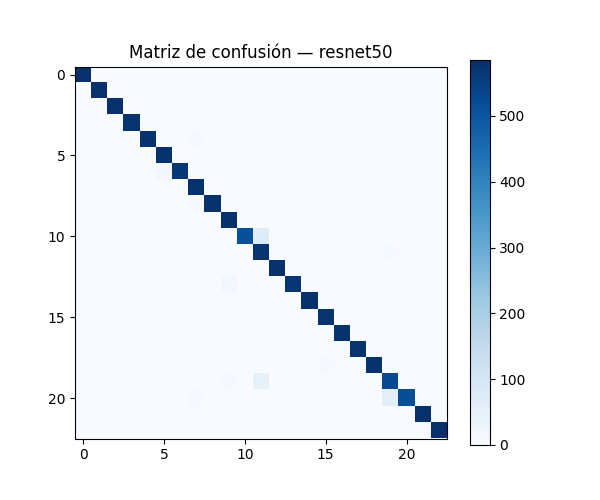
\includegraphics[width=\linewidth]{images/m_rn50.png}
			\caption{Modelo A: ResNet50}
		\end{subfigure}
		\hfill
		\begin{subfigure}{0.48\textwidth}
			\centering
			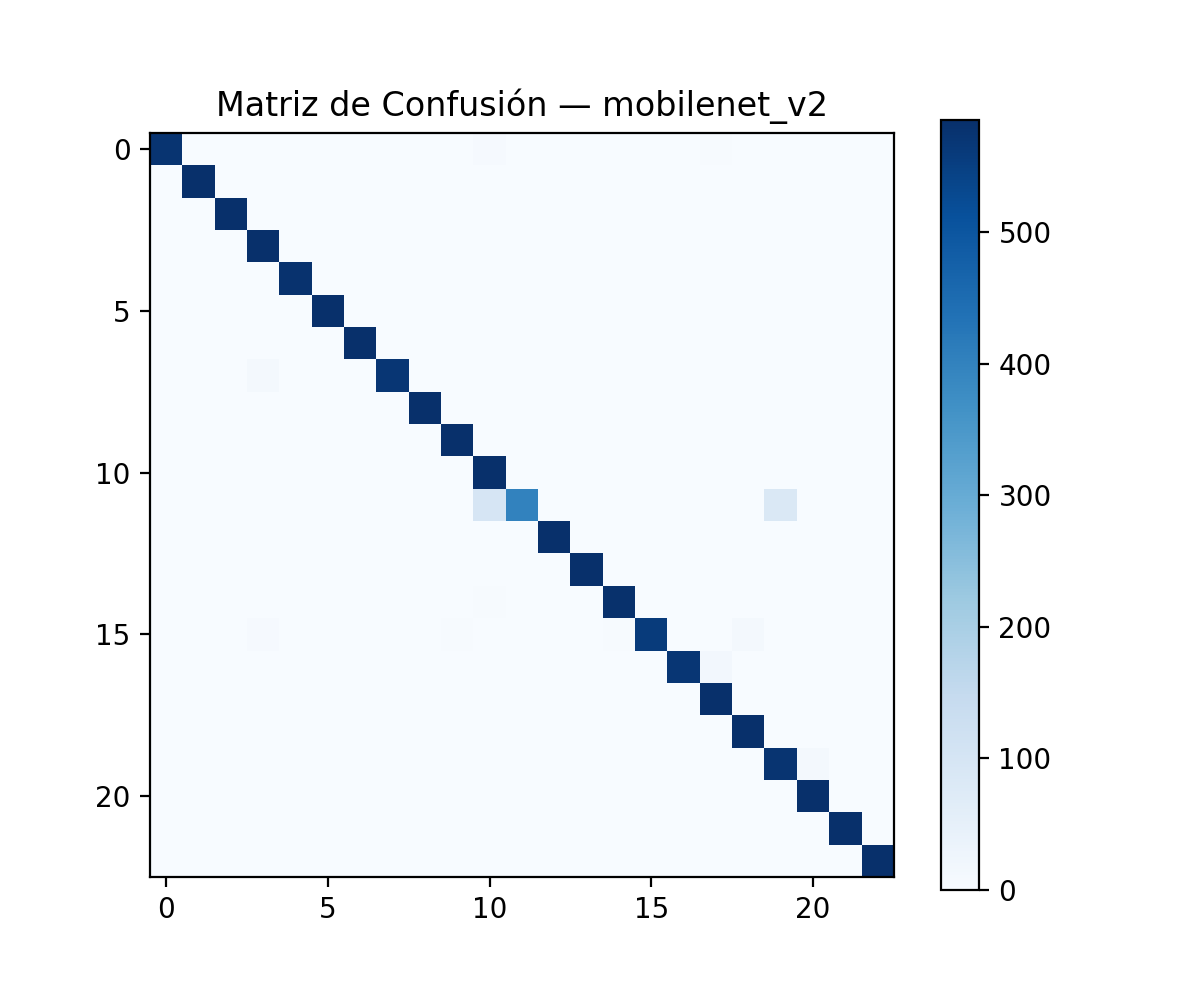
\includegraphics[width=\linewidth]{images/m_mn2.png}
			\caption{Modelo B: MobileNetV2}
		\end{subfigure}
		
		\vspace{0.3cm}
		
		\begin{subfigure}{0.48\textwidth}
			\centering
			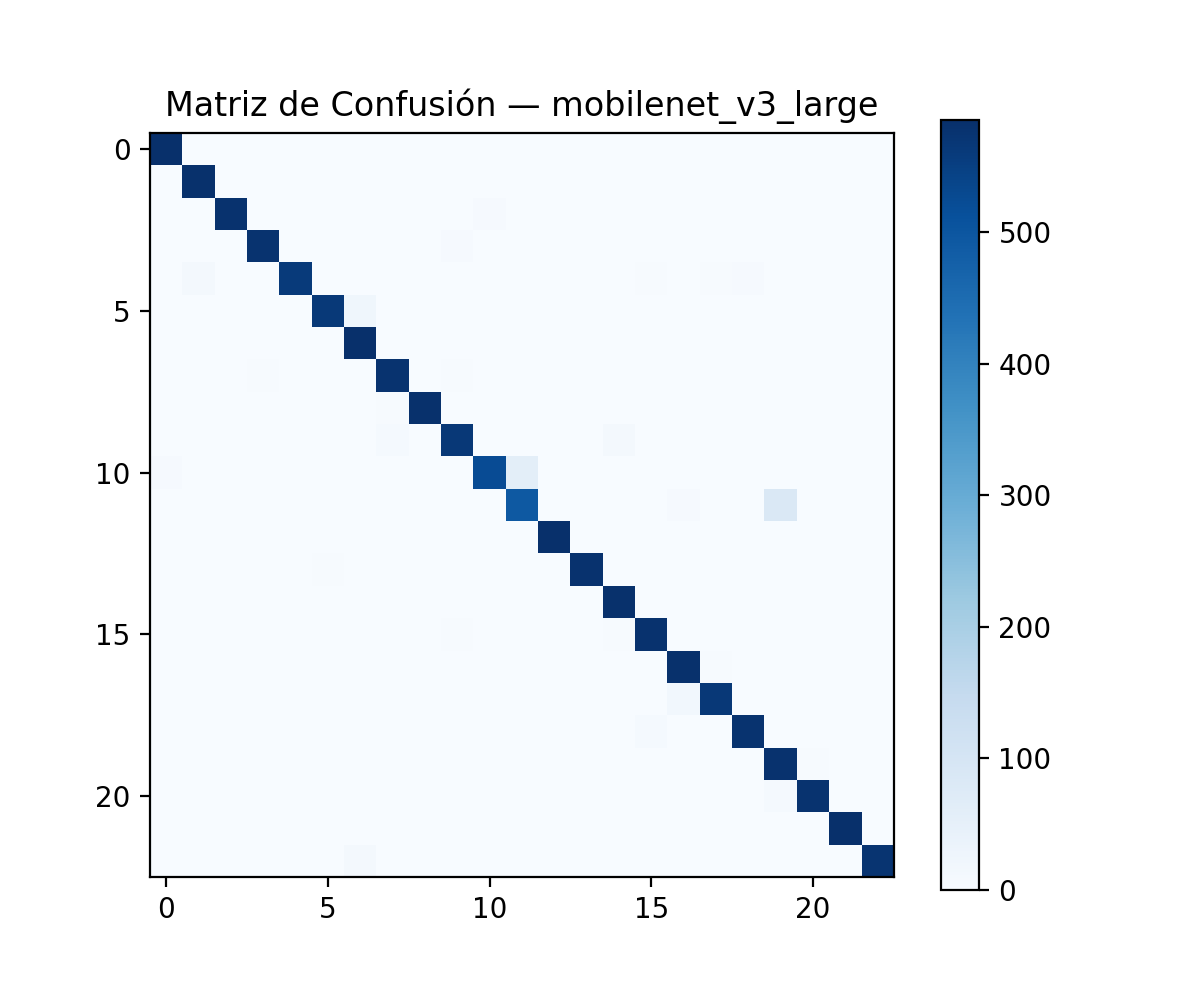
\includegraphics[width=\linewidth]{images/m_mn3.png}
			\caption{Modelo C: MobileNetV3}
		\end{subfigure}
		\hfill
		\begin{subfigure}{0.48\textwidth}
			\centering
			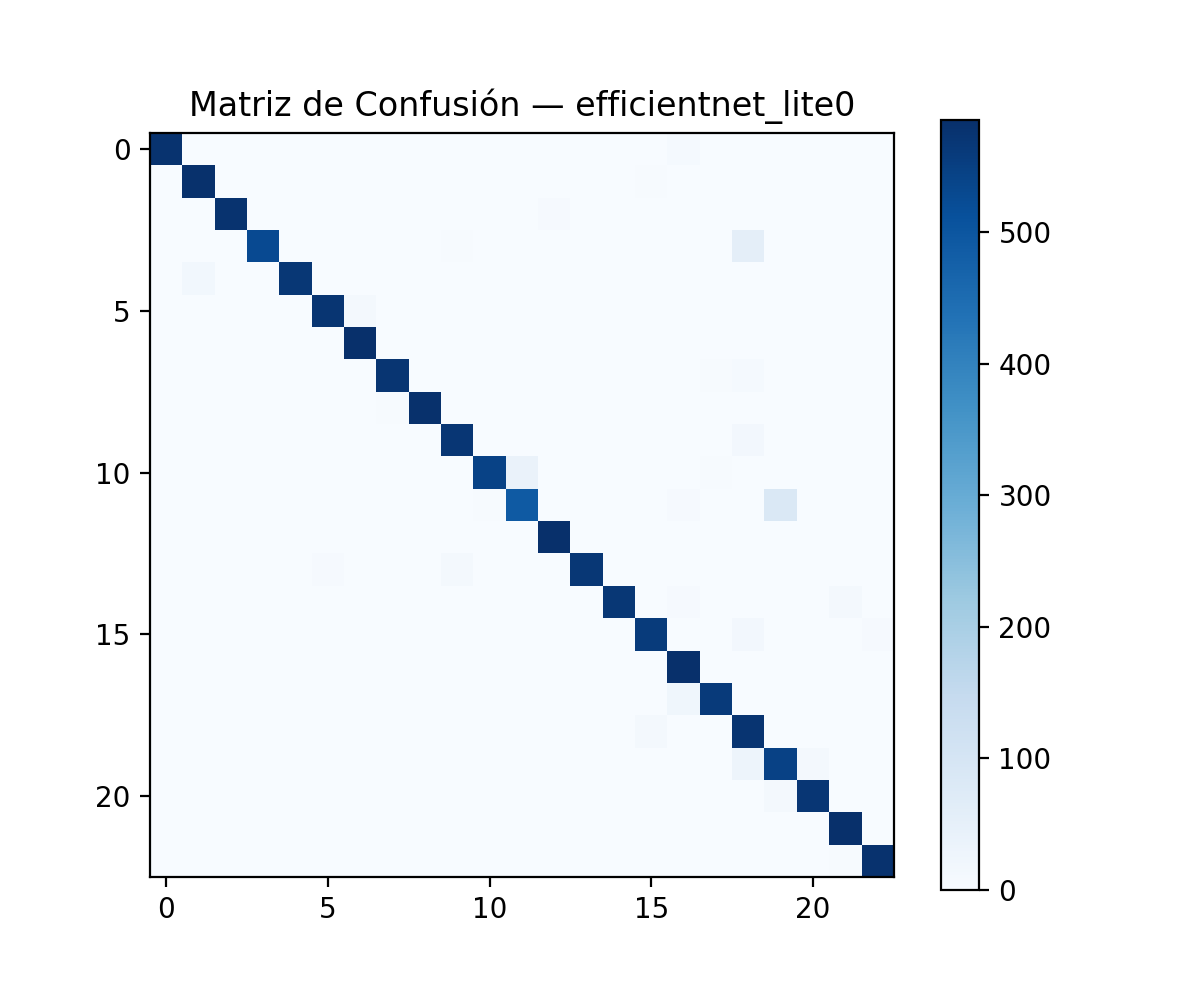
\includegraphics[width=\linewidth]{images/m_en0.png}
			\caption{Modelo D: EfficientNet Lite0}
		\end{subfigure}
		
		\vspace{0.3cm}
		
		\begin{subfigure}{0.48\textwidth}
			\centering
			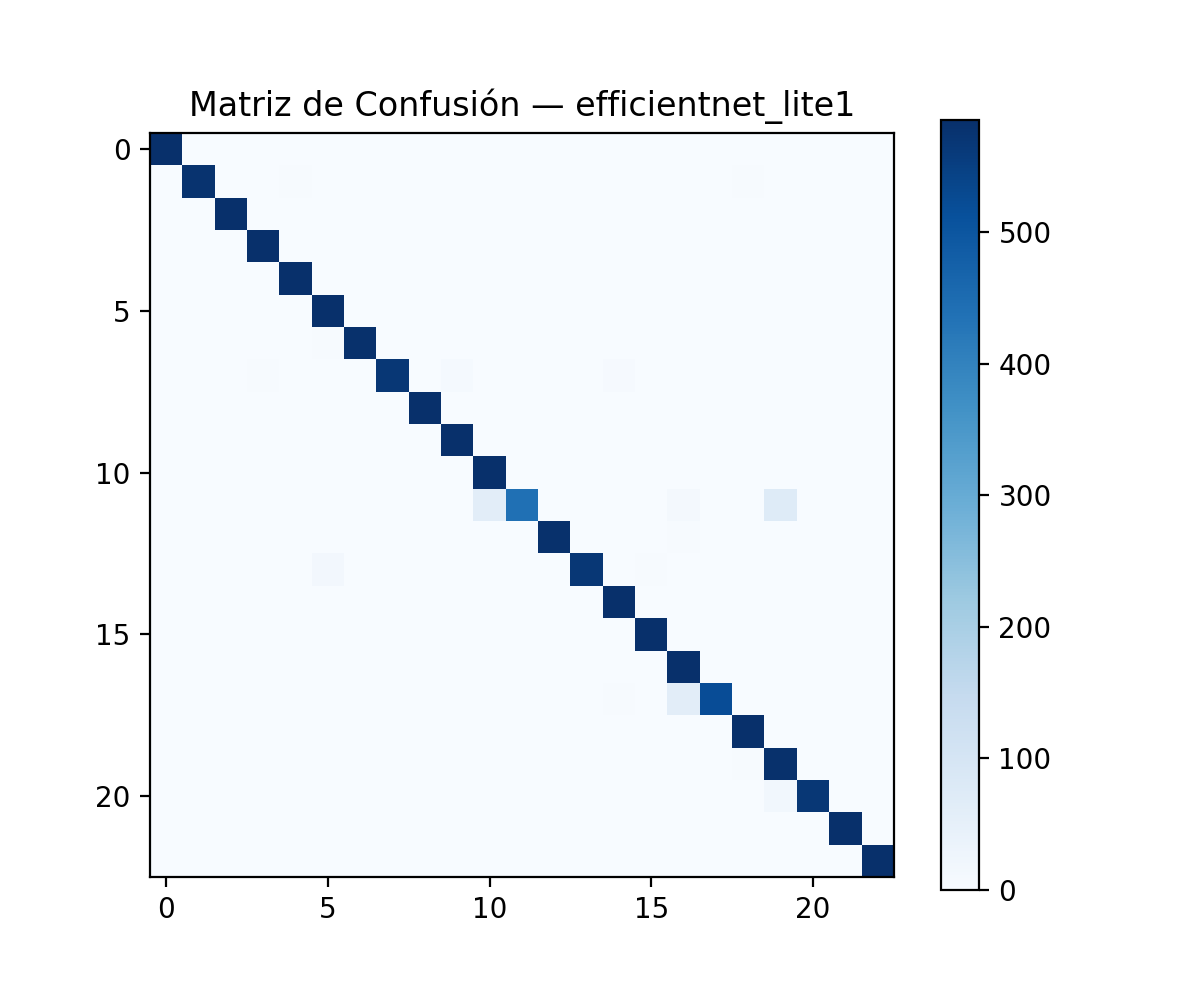
\includegraphics[width=\linewidth]{images/m_en1.png}
			\caption{Modelo E: EfficientNet Lite1}
		\end{subfigure}
		
		\caption{Matrices de confusión obtenidas para las CNN.}
		\label{fig:cnn_confusion}
	\end{figure}
	
	\paragraph{Landmarks}\mbox{}\\
	
	También se presentan las matrices de confusión obtenidas por los modelos basados en landmarks extraídos mediante MediaPipe Hands. Estas matrices permiten analizar el comportamiento de las arquitecturas utilizando representaciones geométricas de la mano, facilitando la comparación respecto a los enfoques basados directamente en imágenes RGB y evaluando su capacidad de generalización en las pruebas experimentales.
	
	\begin{figure}[H]
		\centering
		
		\begin{subfigure}{0.48\textwidth}
			\centering
			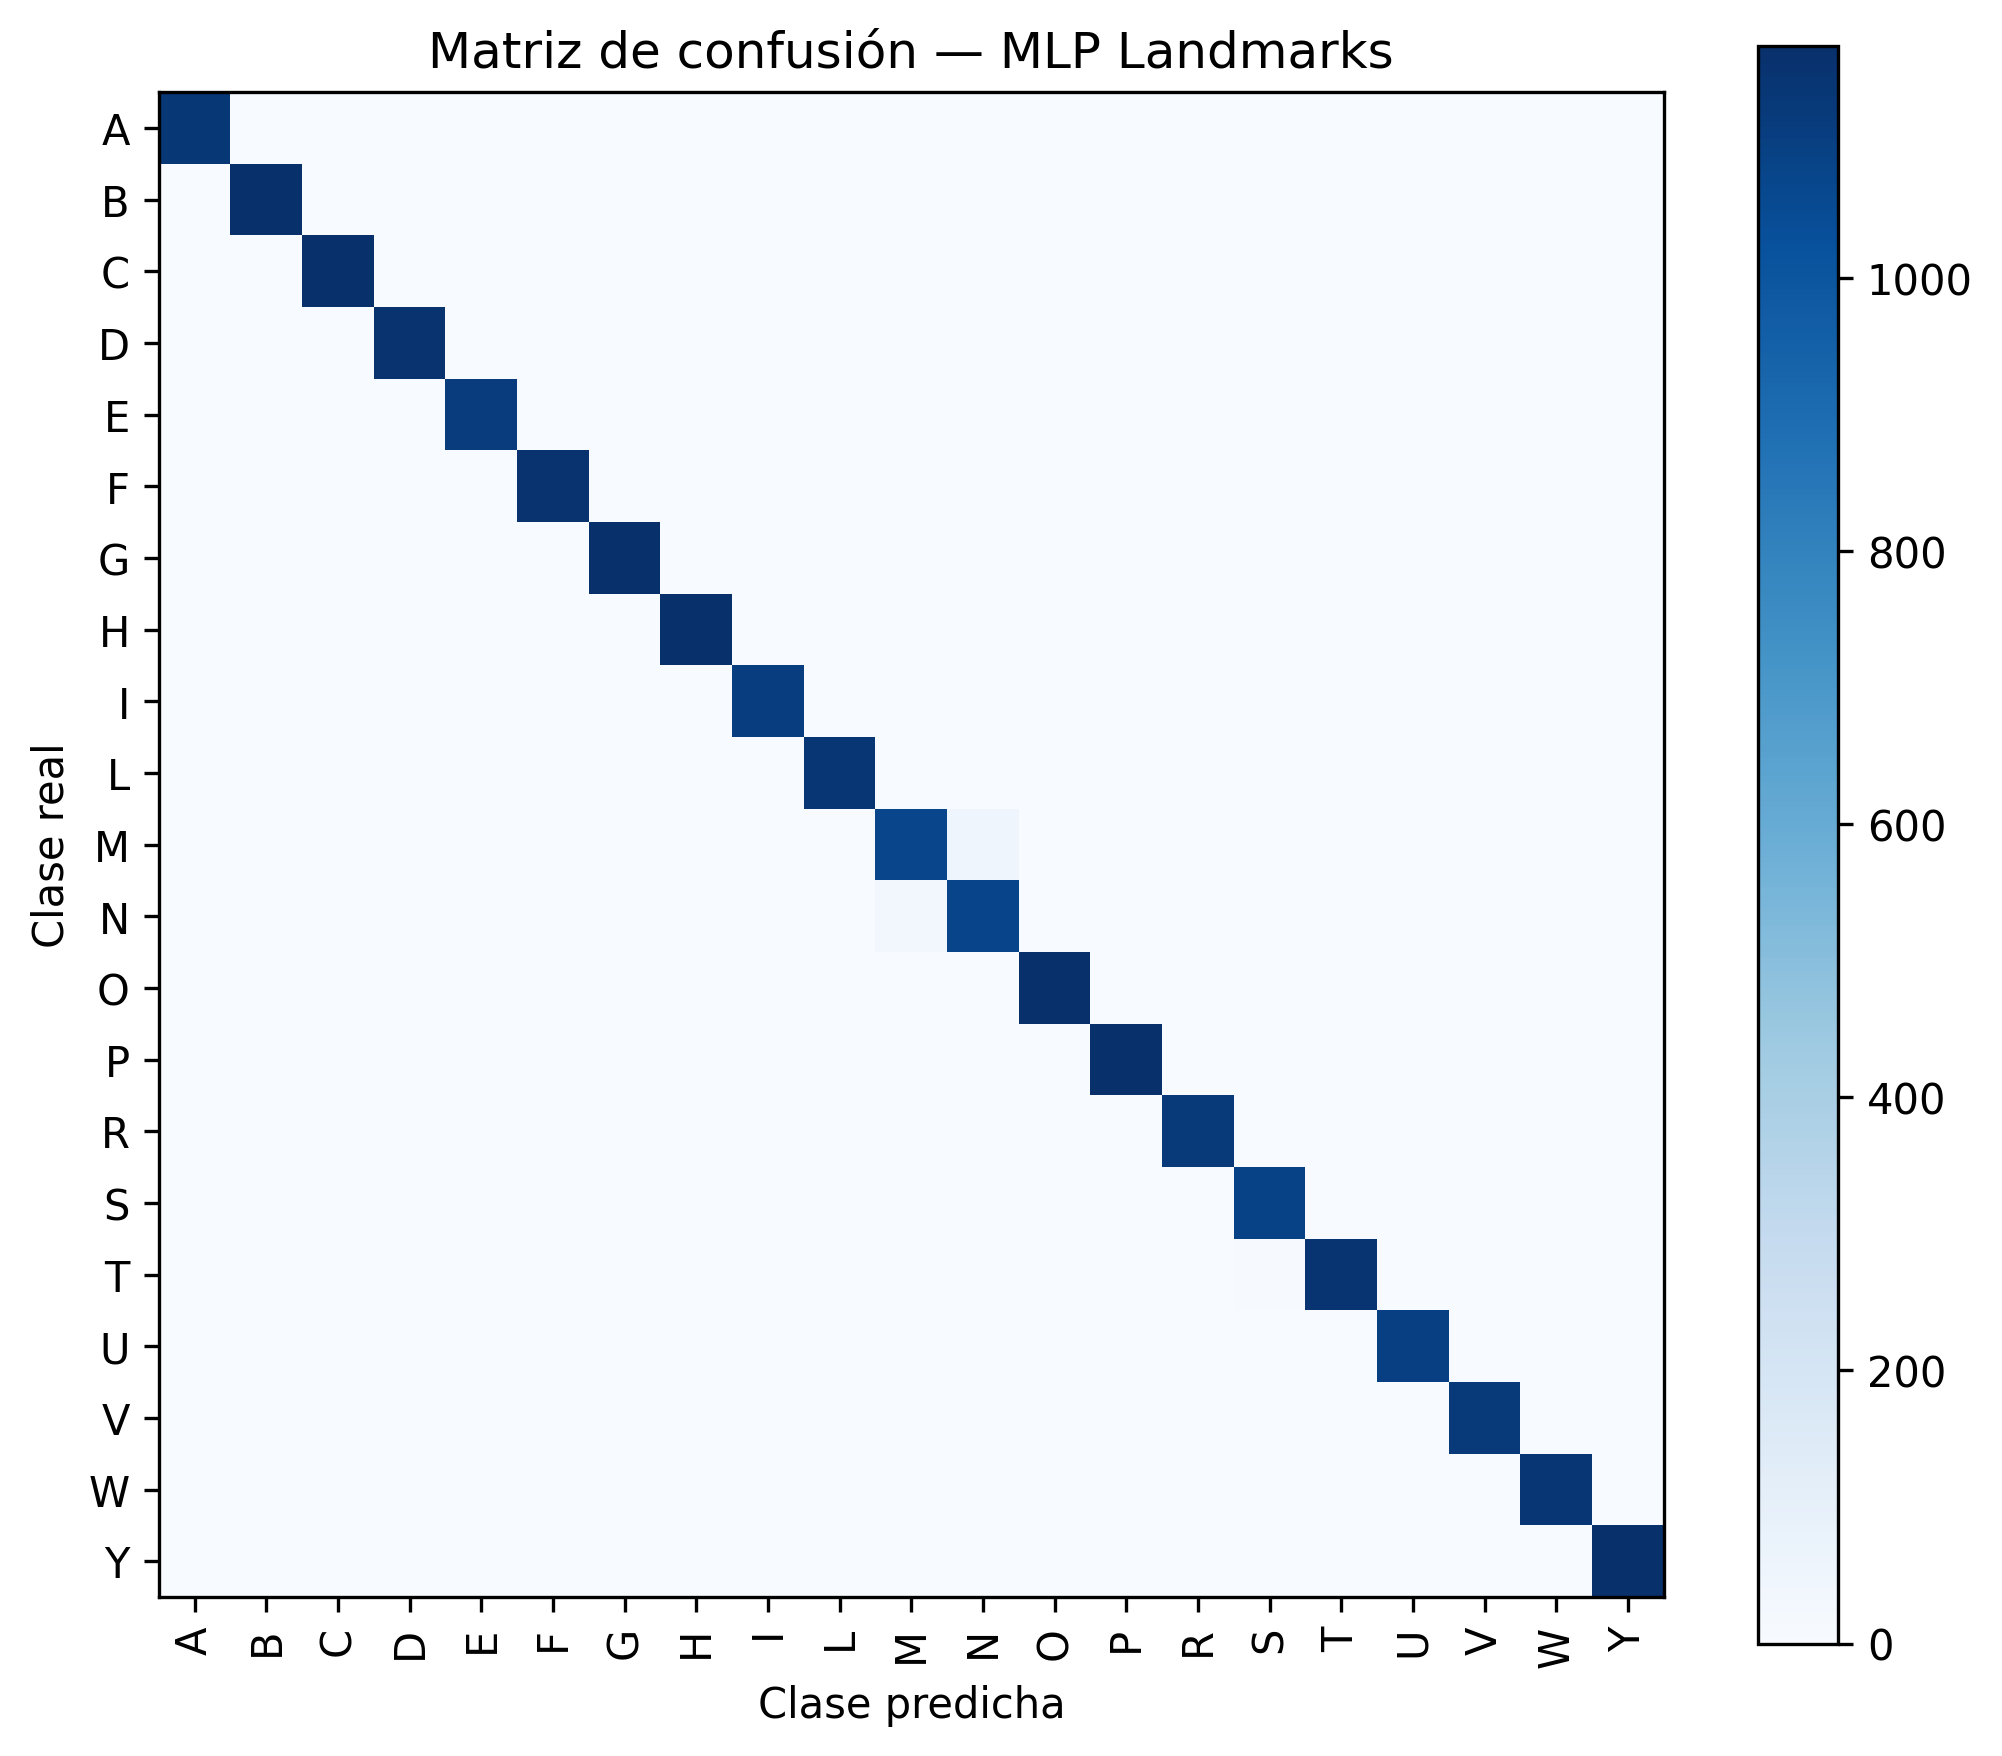
\includegraphics[width=\linewidth]{images/confusion_mlp.png}
			\caption{Modelo A: MLP Landmarks}
		\end{subfigure}
		\hfill
		\begin{subfigure}{0.48\textwidth}
			\centering
			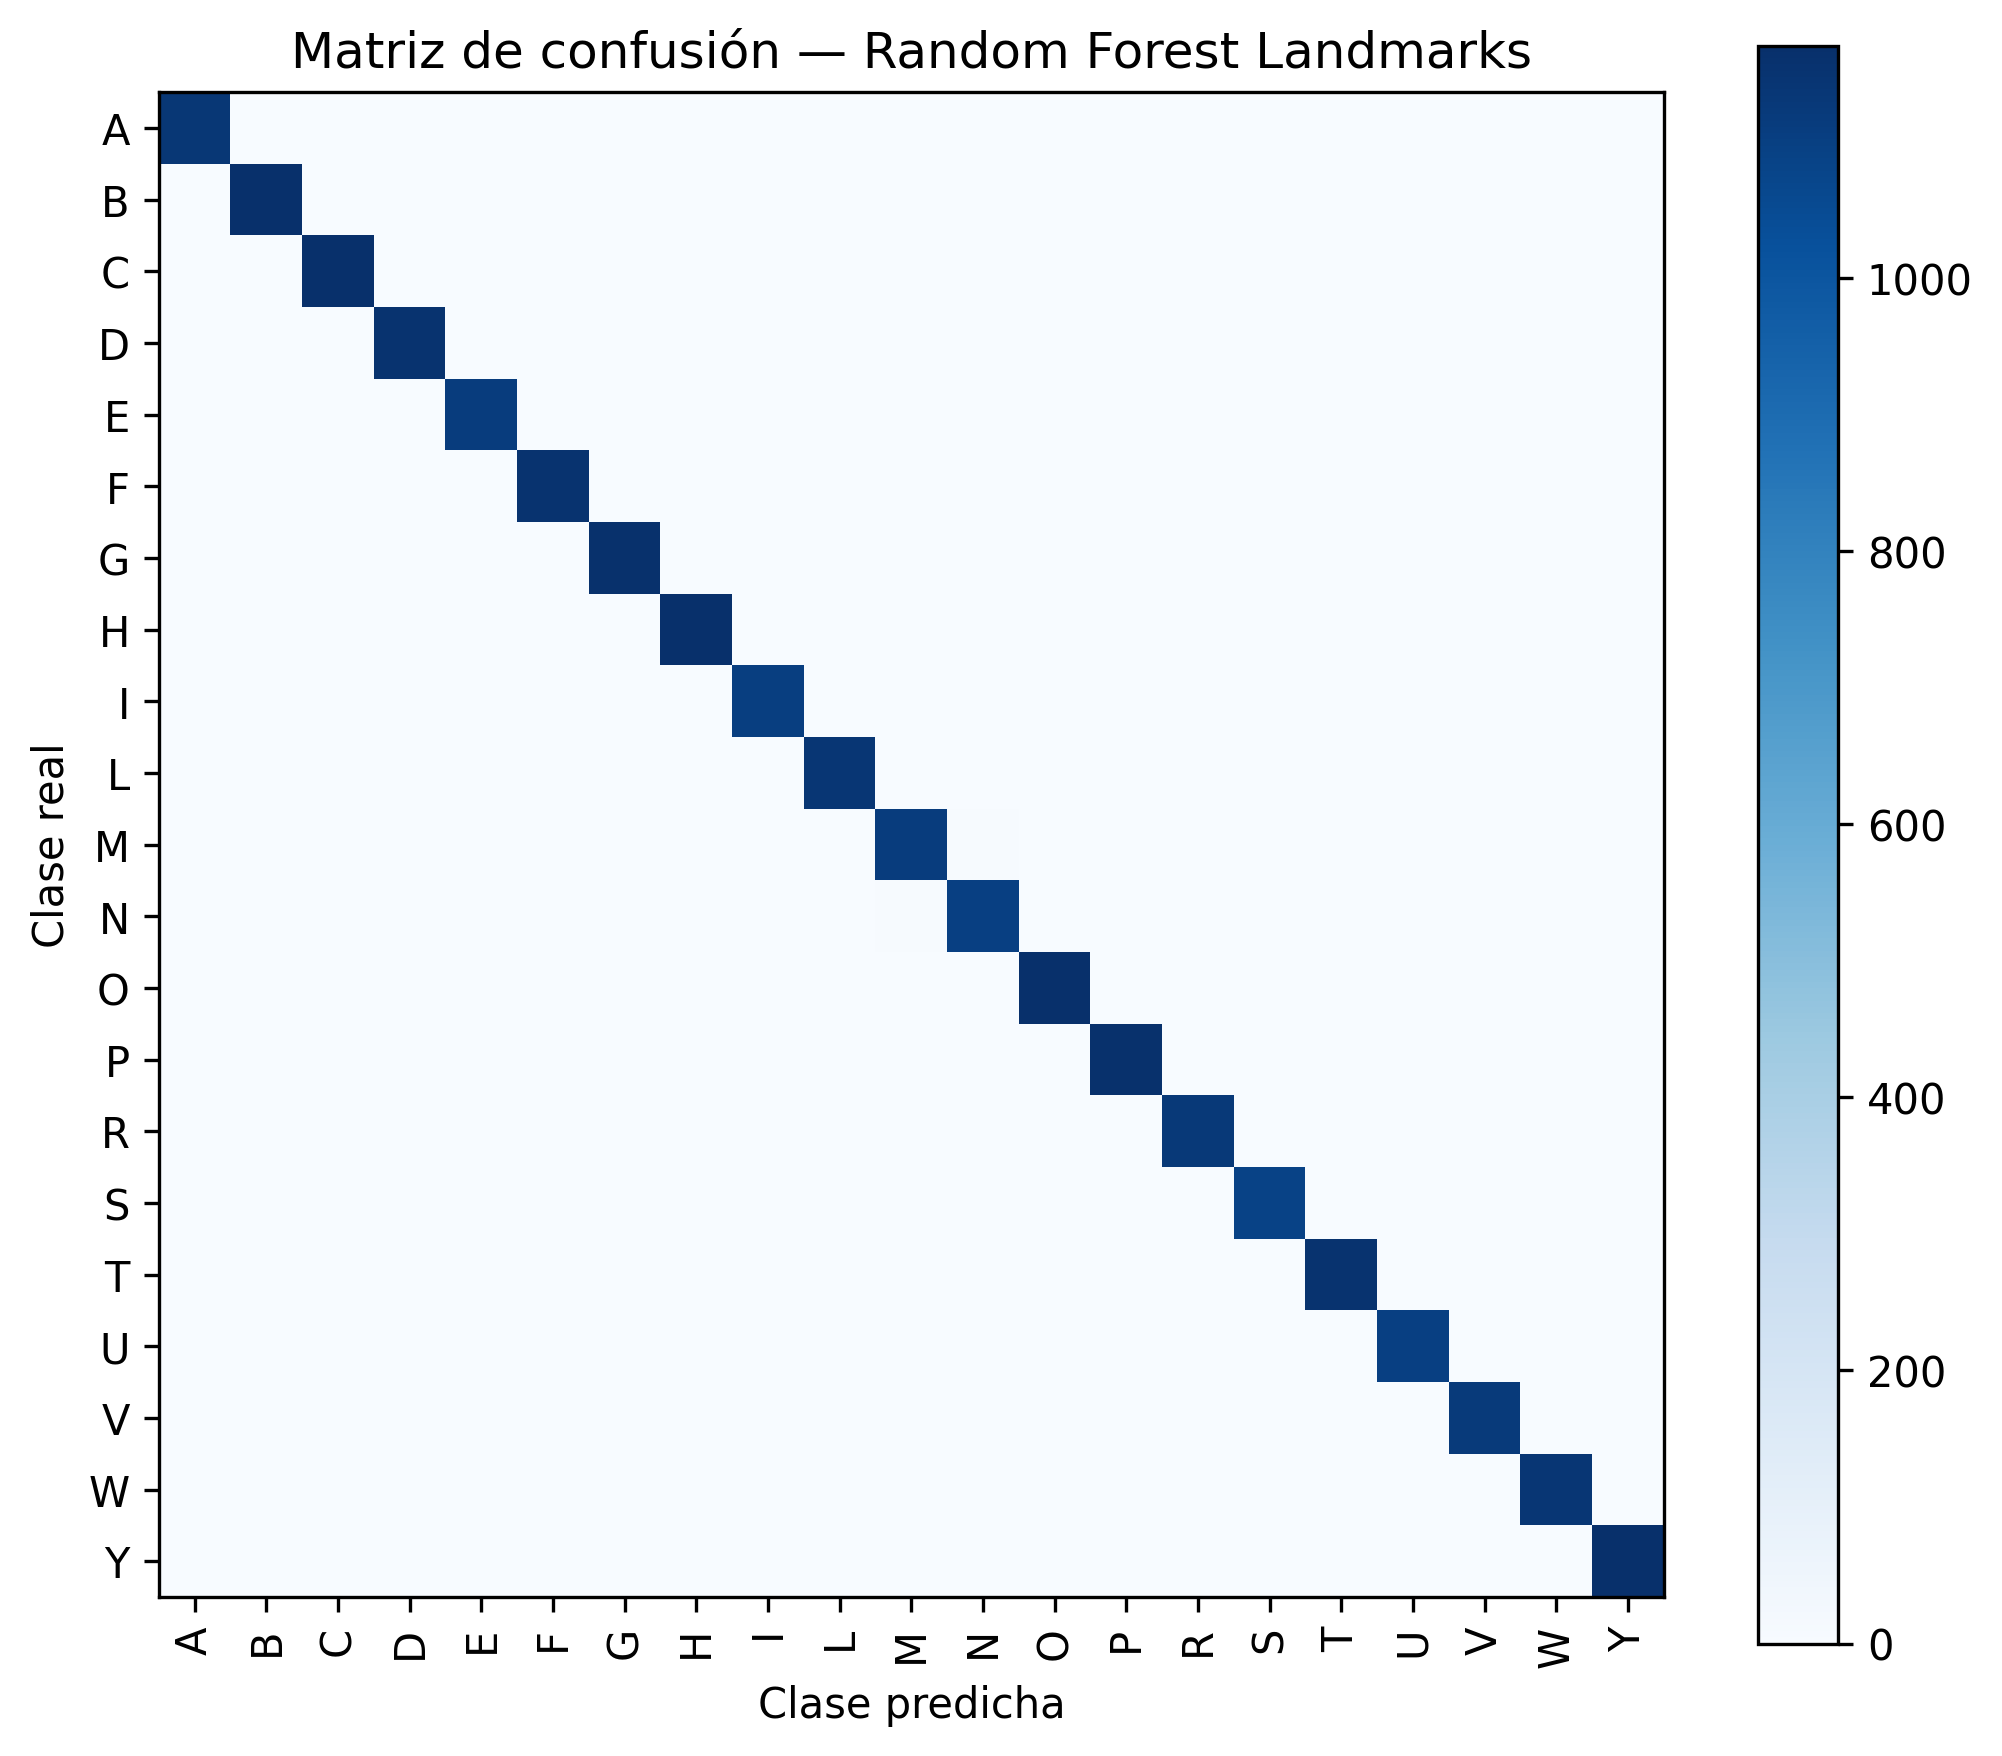
\includegraphics[width=\linewidth]{images/confusion_random_forest.png}
			\caption{Modelo B: Random Forest Landmarks}
		\end{subfigure}
		
		\vspace{0.3cm}
		
		\begin{subfigure}{0.48\textwidth}
			\centering
			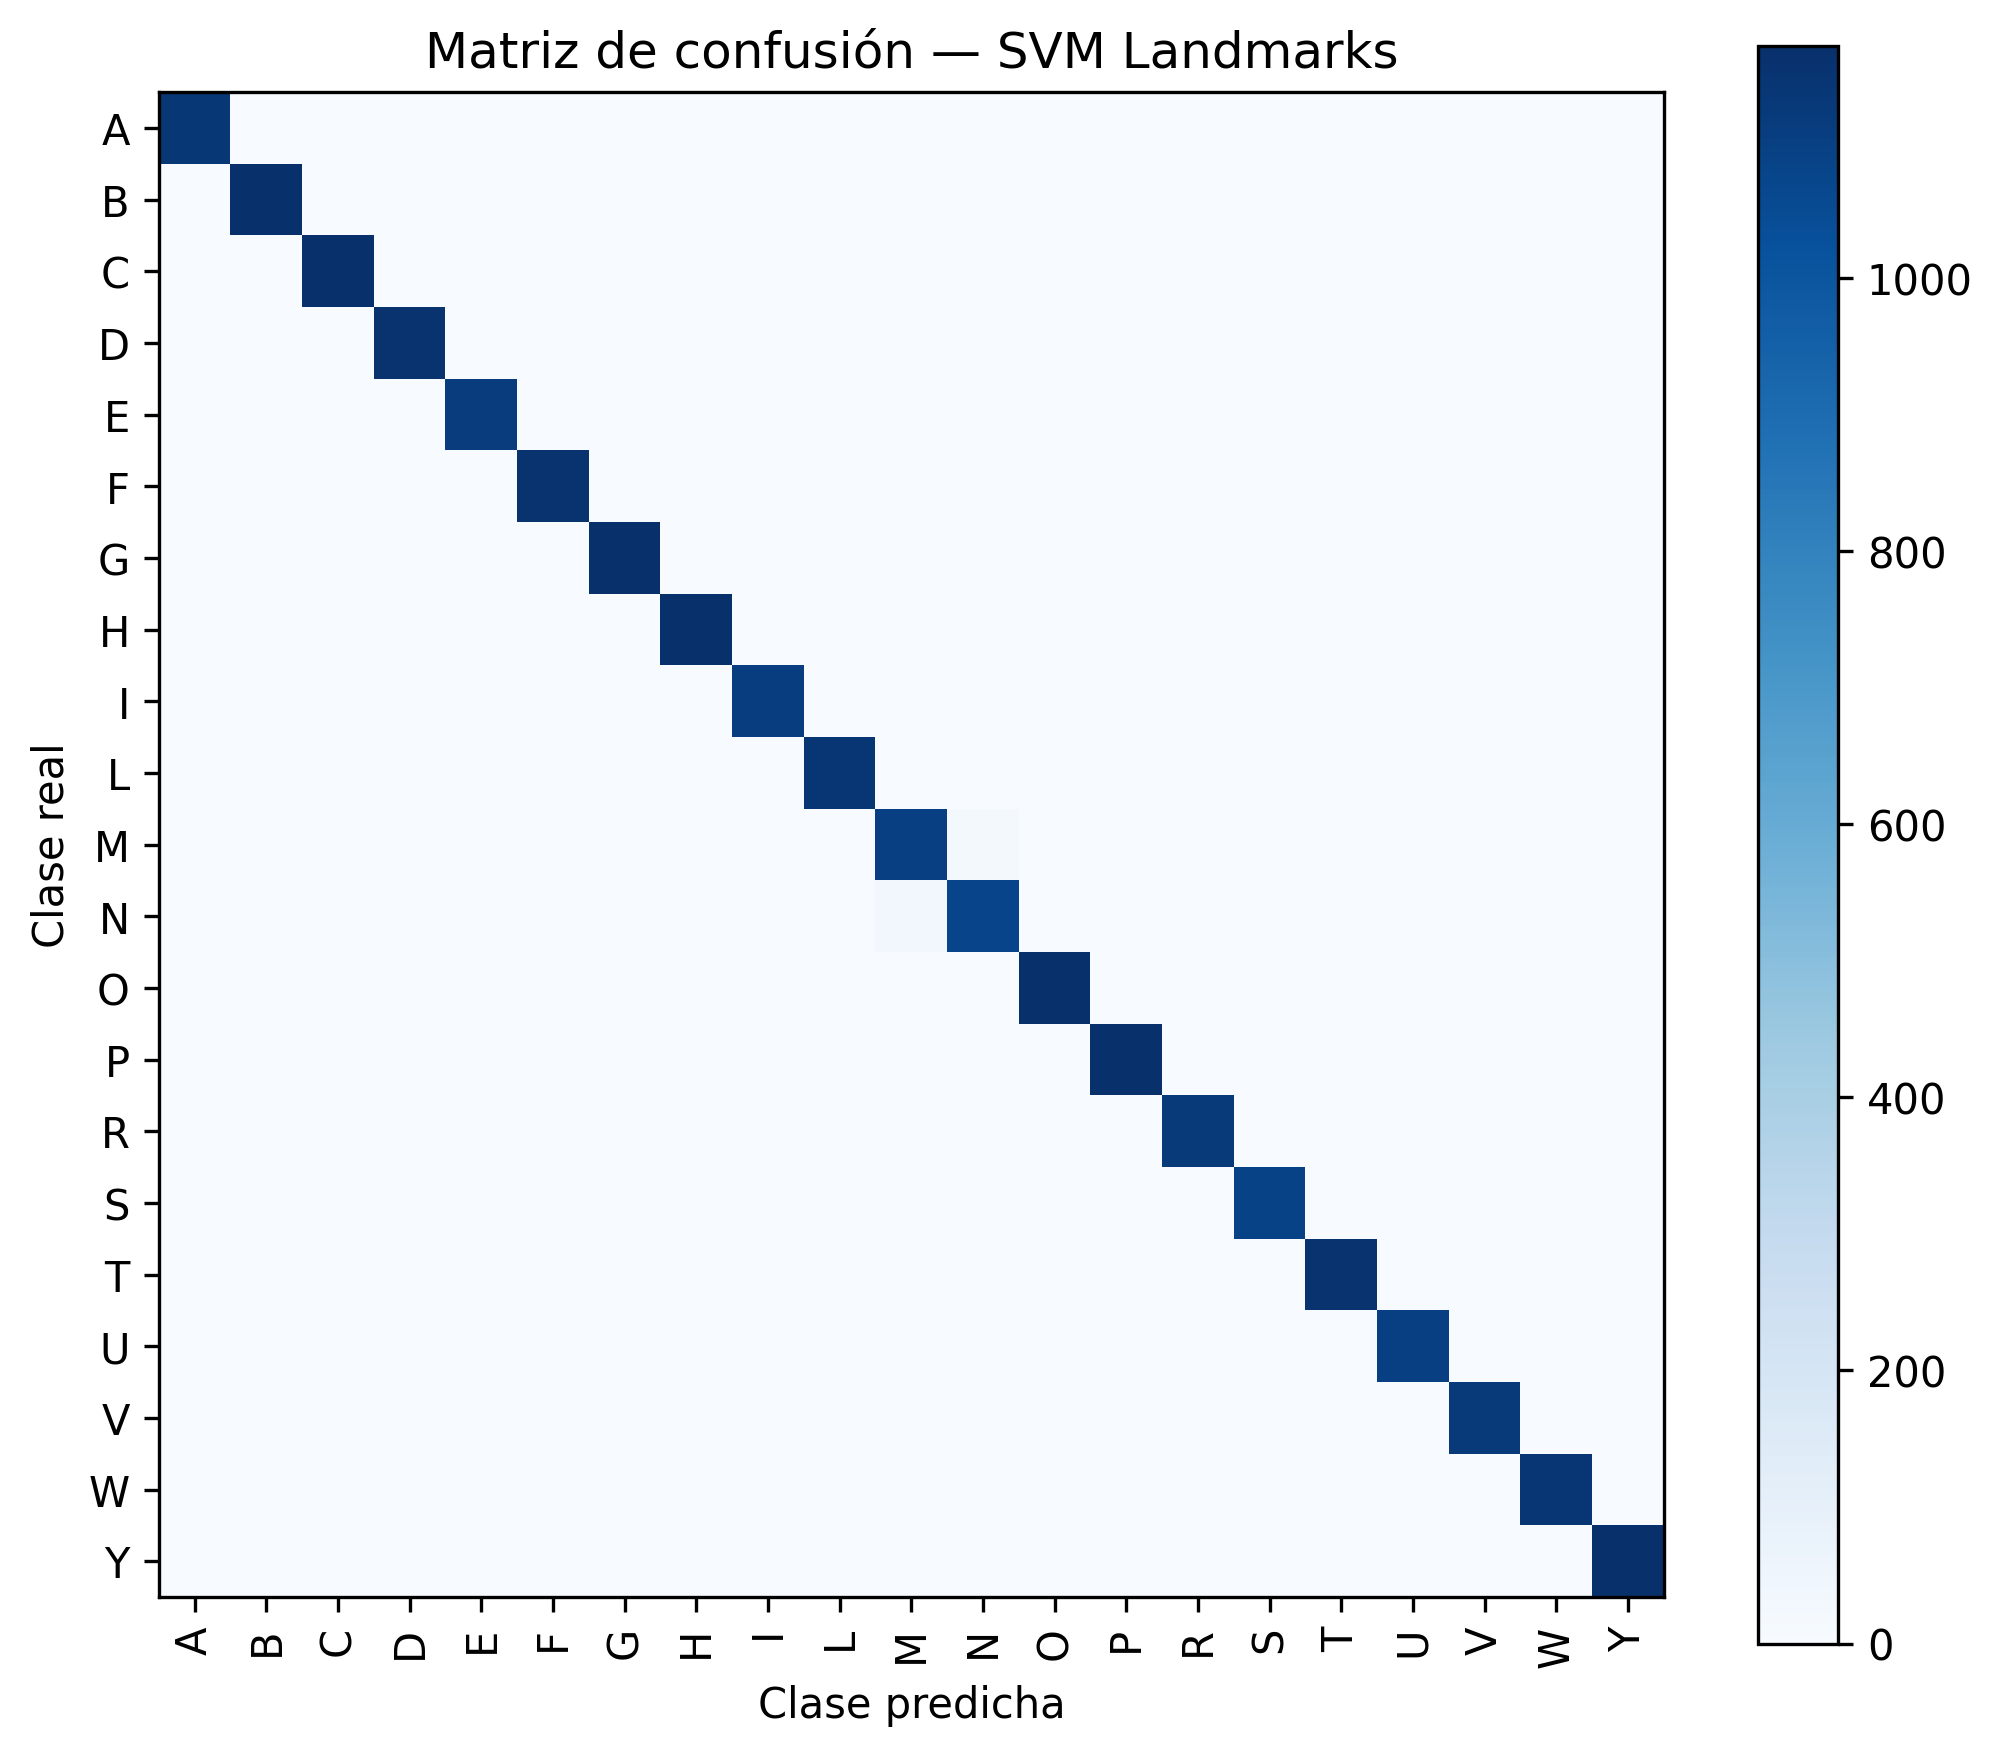
\includegraphics[width=\linewidth]{images/confusion_svm.png}
			\caption{Modelo C: SVM Landmarks}
		\end{subfigure}
		
		\caption{Matrices de confusión obtenidas para los modelos basados en landmarks extraídos mediante MediaPipe Hands.}
		\label{fig:landmarks_confusion}
	\end{figure}
	
	
	\paragraph{Interpretación general de las matrices de confusión}\mbox{}\\
	
	Las matrices de confusión obtenidas en las pruebas experimentales permitieron analizar de manera más detallada el comportamiento de clasificación de las diferentes arquitecturas evaluadas, identificando tanto los patrones generales de acierto como las principales clases con tendencia a confusión \cite{goodfellow2016deep,geron2022hands}.
	
	En términos generales todas las arquitecturas presentaron una concentración dominante sobre la diagonal principal de las matrices, lo cual indica que la mayoría de las muestras fueron clasificadas correctamente.
	
	En el caso de las CNN basadas en imágenes RGB, las matrices mostraron un desempeño considerablemente estable para la mayoría de las clases evaluadas. Modelos como ResNet50, MobileNetV2 y EfficientNet Lite1 presentaron diagonales claramente definidas y una baja dispersión de errores fuera de la diagonal principal, evidenciando una adecuada capacidad de aprendizaje sobre el conjunto de entrenamiento y prueba.
	
	Aunque las métricas globales resultaron elevadas, las matrices de confusión permitieron observar que ciertas clases continuaban presentando errores ocasionales de clasificación. Particularmente, algunas señas con configuraciones de mano similares tendieron a generar pequeñas regiones de confusión entre determinadas categorías. Estas situaciones fueron visibles en clases cuya geometría dependía de variaciones sutiles en la posición de dedos individuales o en pequeñas diferencias angulares de la mano.
	
	Las arquitecturas basadas directamente en imágenes RGB mostraron una mayor sensibilidad frente a variaciones externas presentes en la captura de imágenes, incluyendo cambios de iluminación, orientación de la mano, distancia respecto a la cámara y complejidad del fondo..
	
	Las matrices correspondientes a los modelos basados en landmarks presentaron una diagonal principal todavía más dominante y una cantidad considerablemente menor de errores dispersos entre clases. Particularmente, los modelos SVM Landmarks y MLP Landmarks mostraron un comportamiento altamente consistente, manteniendo clasificaciones correctas incluso en clases que anteriormente generaban pequeñas regiones de confusión en los enfoques basados en imágenes RGB.
	
	Estos resultados podrían indicar  que la representación geométrica obtenida mediante MediaPipe Hands permitió abstraer gran parte de la información irrelevante presente en las imágenes originales, enfocando el proceso de clasificación principalmente sobre la estructura espacial de la mano y la relación entre articulaciones \cite{mediapipe}.
	
	Otro aspecto importante observado mediante las matrices de confusión fue la capacidad de generalización alcanzada por los modelos basados en landmarks. Mientras que algunas arquitecturas de CNN tendían a depender parcialmente de características visuales asociadas al entorno de captura, los modelos geométricos mantuvieron un comportamiento considerablemente más estable al trabajar únicamente con coordenadas espaciales normalizadas.
	
	
	\paragraph{Clases con mayor confusión}\mbox{}\\
	
	El análisis detallado de las matrices de confusión permitió identificar que, aunque el desempeño global de los modelos fue considerablemente elevado, ciertas clases continuaron presentando tendencias de confusión recurrentes debido a similitudes geométricas y visuales entre determinadas señas del alfabeto de LSM.
	
	En las CNN, las principales regiones de error se concentraron particularmente entre las letras \textit{M}, \textit{N}, \textit{U}, \textit{V} y, en menor medida, \textit{S} y \textit{T}. Estas clases presentaron reducciones visibles en métricas como \textit{recall} y \textit{precision}, indicando que algunas muestras fueron clasificadas incorrectamente como otras categorías visualmente similares.
	
	Particularmente, la letra \textit{N} representó una de las clases más complejas para las CNN. En EfficientNet Lite0, esta clase obtuvo un recall aproximado de 83.76\%, mientras que en MobileNetV2 descendió incluso hasta valores cercanos al 68.03\%. Este rendimiento indica que una parte importante de muestras reales pertenecientes a la clase \textit{N} fueron clasificadas erróneamente como otras señas similares.
	
	Algo muy similar ocurrió en las letras \textit{U} y \textit{V} presentaron dificultades importantes en diversos modelos convolucionales. En EfficientNet Lite0, la precisión de la clase \textit{U} descendió hasta aproximadamente 82.14\%, mientras que la clase \textit{V} obtuvo una precisión cercana al 84.60\%. Resultados similares también fueron observados en MobileNetV2 y MobileNetV3, donde las métricas asociadas a la clase \textit{V} permanecieron consistentemente por debajo de otras categorías.
	
	Estas confusiones pueden explicarse debido a que las señas mencionadas poseen configuraciones de mano altamente similares, diferenciándose únicamente por pequeñas variaciones en la cantidad de dedos extendidos, separación angular o posición relativa del pulgar. Como consecuencia, pequeñas variaciones de iluminación, orientación de cámara o movimiento de la mano podían alterar significativamente las características visuales aprendidas por las CNN.
	
	Por otra parte, las matrices de confusión correspondientes a los modelos basados en landmarks mostraron una reducción considerable en la dispersión de errores. En particular, SVM Landmarks presentó el comportamiento más estable y consistente entre todos los modelos evaluados, alcanzando una exactitud global superior al 99\%.
	
	Aun así incluso los modelos geométricos basados en landmarks conservaron pequeñas regiones de confusión entre las clases \textit{M} y \textit{N}. Estas dos señas continuaron representando el principal desafío de clasificación debido a la similitud estructural inherente entre ambas configuraciones manuales. Por ejemplo, en MLP Landmarks la clase \textit{N} presentó un recall aproximado de 90.62\% mientras que la clase \textit{M} obtuvo una precisión cercana al 91.17\%.
	
	Random Forest Landmarks presentó ligeras confusiones adicionales entre las letras \textit{S}, \textit{T}, \textit{U} y \textit{V}, aunque con una magnitud considerablemente menor respecto a los modelos convolucionales. Estas diferencias sugieren que, aun cuando la representación geométrica mejora significativamente la robustez del sistema, algunas señas continúan siendo naturalmente difíciles de separar debido a la similitud física de las posiciones articulares.
	
	
	Este análisis de las clases con mayor confusión permitió identificar las señas que representan un mayor reto para el prototipo actual de reconocimiento de señas, proporcionando información importante para futuras etapas de optimización, ampliación del conjunto de datos y mejora de estrategias de normalización e inferencia continua en dispositivos móviles.
	
	
	{
		\rowcolors{2}{rowblue}{white}
		
		\small
		\renewcommand{\arraystretch}{1.15}
		
		\begin{table}[H]
			\centering
			\caption{Principales clases con mayor confusión observadas en las pruebas experimentales de los modelos evaluados.}
			\label{tab:clases_confusion}
			
			\resizebox{\textwidth}{!}{
				
				\begin{tabular}{
						!{\vrule width 0.6pt}
						>{\centering\arraybackslash}p{3.2cm}
						!{\vrule width 0.6pt}
						>{\centering\arraybackslash}p{1.2cm}
						!{\vrule width 0.6pt}
						>{\centering\arraybackslash}p{2.4cm}
						!{\vrule width 0.6pt}
						>{\centering\arraybackslash}p{1.8cm}
						!{\vrule width 0.6pt}
						>{\centering\arraybackslash}p{4.8cm}
						!{\vrule width 0.6pt}
					}
					\hline
					
					\rowcolor{headerblue}
					\textcolor{white}{\textbf{Modelo}} &
					\textcolor{white}{\textbf{Clase}} &
					\textcolor{white}{\textbf{Métrica afectada}} &
					\textcolor{white}{\textbf{Valor}} &
					\textcolor{white}{\textbf{Observación}} \\
					
					\hline
					
					MobileNetV2 & N & Recall & 68.03\% & Confusión frecuente con M \\
					\hline
					MobileNetV2 & V & Precision & 86.96\% & Similitud con U \\
					\hline
					MobileNetV2 & R & Recall & 95.38\% & Variaciones de orientación \\
					\hline
					
					MobileNetV3 & N & Precision & 82.68\% & Confusión estructural con M \\
					\hline
					MobileNetV3 & W & Recall & 88.37\% & Configuración de dedos similar \\
					\hline
					MobileNetV3 & V & Recall & 89.91\% & Separación angular limitada \\
					\hline
					
					ResNet50 & N & Recall & 84.27\% & Dificultad de separación con M \\
					\hline
					ResNet50 & M & Recall & 89.23\% & Posición parcial de dedos \\
					\hline
					ResNet50 & V & Precision & 86.05\% & Variaciones geométricas \\
					\hline
					
					EfficientNet Lite0 & U & Precision & 82.14\% & Confusión con V \\
					\hline
					EfficientNet Lite0 & N & Recall & 83.76\% & Alta similitud gestual \\
					\hline
					EfficientNet Lite0 & M & Recall & 89.57\% & Sensibilidad a orientación \\
					\hline
					
					EfficientNet Lite1 & N & Recall & 68.03\% & Confusión recurrente con M \\
					\hline
					EfficientNet Lite1 & V & Precision & 86.97\% & Variaciones de dedos \\
					\hline
					EfficientNet Lite1 & S & Recall & 97.43\% & Pequeñas diferencias articulares \\
					\hline
					
					MLP Landmarks & N & Recall & 90.62\% & Confusión parcial con M \\
					\hline
					MLP Landmarks & M & Precision & 91.17\% & Similitud geométrica \\
					\hline
					MLP Landmarks & V & Recall & 95.89\% & Separación angular reducida \\
					\hline
					
					Random Forest & U & Recall & 91.66\% & Variaciones de orientación \\
					\hline
					Random Forest & S & Precision & 95.16\% & Configuración similar con T \\
					\hline
					Random Forest & N & Recall & 92.30\% & Diferencias gestuales sutiles \\
					\hline
					
					SVM Landmarks & N & Recall & 90.62\% & Confusión parcial con M \\
					\hline
					SVM Landmarks & M & Precision & 91.17\% & Posición similar de dedos \\
					\hline
					SVM Landmarks & V & Recall & 95.89\% & Diferencias geométricas pequeñas \\
					\hline
					
				\end{tabular}
				
			}
		\end{table}
	}
		
	
	\paragraph{Resultados de inferencia en PC}\mbox{}\\
	{
		\rowcolors{2}{rowblue}{white}
		
		\small
		\renewcommand{\arraystretch}{1.15}
		
		\begin{table}[H]
			\centering
			\caption{Resultados de inferencia en PC obtenidos mediante pruebas experimentales utilizando imágenes externas al conjunto de entrenamiento.}
			\label{tab:inferencia_pc_cnn}
			
			\resizebox{\textwidth}{!}{
				
				\begin{tabular}{
						!{\vrule width 0.6pt}
						>{\centering\arraybackslash}p{3.6cm}
						!{\vrule width 0.6pt}
						>{\centering\arraybackslash}p{1.8cm}
						!{\vrule width 0.6pt}
						>{\centering\arraybackslash}p{1.0cm}
						!{\vrule width 0.6pt}
						>{\centering\arraybackslash}p{1.0cm}
						!{\vrule width 0.6pt}
						>{\centering\arraybackslash}p{1.0cm}
						!{\vrule width 0.6pt}
						>{\centering\arraybackslash}p{1.0cm}
						!{\vrule width 0.6pt}
						>{\centering\arraybackslash}p{1.0cm}
						!{\vrule width 0.6pt}
					}
					\hline
					
					\rowcolor{headerblue}
					\textcolor{white}{\textbf{Modelo}} &
					\textcolor{white}{\textbf{Acc Global}} &
					\textcolor{white}{\textbf{A}} &
					\textcolor{white}{\textbf{E}} &
					\textcolor{white}{\textbf{I}} &
					\textcolor{white}{\textbf{O}} &
					\textcolor{white}{\textbf{U}} \\
					
					\hline
					
					MobileNetV2 &
					4\% &
					0\% &
					0\% &
					0\% &
					20\% &
					0\% \\
					\hline
					
					ResNet50 &
					44\% &
					60\% &
					0\% &
					60\% &
					100\% &
					0\% \\
					\hline
					
					EfficientNet Lite1 &
					36\% &
					80\% &
					0\% &
					0\% &
					100\% &
					0\% \\
					\hline
					
					MobileNetV3 &
					23\% &
					20\% &
					0\% &
					0\% &
					100\% &
					0\% \\
					\hline
					
					EfficientNet Lite0 &
					36\% &
					80\% &
					0\% &
					0\% &
					100\% &
					0\% \\
					\hline
					
				\end{tabular}
				
			}
		\end{table}
	}
	
	
	Para evaluar la capacidad de generalización de las CNNs fuera del conjunto de entrenamiento, se realizaron pruebas de inferencia en computadora utilizando imágenes y capturas externas no incluidas previamente en el entrenamiento del modelo. Para esta evaluación se seleccionaron inicialmente las vocales del alfabeto (\textit{A}, \textit{E}, \textit{I}, \textit{O} y \textit{U}), debido a que representan algunas de las señas más sencillas y visualmente diferenciables dentro del conjunto de datos.

	Cada seña fue evaluada experimentalmente en 20 ocasiones por modelo, utilizando variaciones reales de posición, distancia, orientación y condiciones de iluminación respecto al entorno controlado originalmente utilizado en la adquisición del dataset.
	
	Los resultados obtenidos evidenciaron una disminución considerable en el desempeño de las arquitecturas CNN en las pruebas reales de inferencia. Aunque modelos como MobileNetV2, EfficientNet Lite1 y ResNet50 habían alcanzado métricas superiores al 97\% en validación y prueba sobre el dataset, su comportamiento en clasificación continua mostró una capacidad de generalización significativamente limitada.
	
	MobileNetV2 presentó un desempeño global aproximado del 4\%, siendo incapaz de reconocer correctamente la mayoría de las vocales evaluadas. Algo parecido ocurrio con  MobileNetV3 y EfficientNet Lite0 mostraron resultados inferiores al esperado, obteniendo precisiones globales aproximadas de 23\% y 36\%, respectivamente.
	
	Incluso modelos más robustos como ResNet50 únicamente alcanzaron un desempeño cercano al 44\%, mostrando además una fuerte dependencia respecto a ciertas configuraciones visuales específicas presentes durante el entrenamiento original. En la mayoría de los modelos se observó que únicamente la vocal \textit{O} mantenía porcentajes de reconocimiento elevados, mientras que clases como \textit{E} y \textit{U} presentaron tasas de reconocimiento prácticamente nulas.
	
	Se observó que la calidad, diversidad y robustez del conjunto de datos utilizado en el entrenamiento influían directamente sobre la capacidad de generalización del modelo. Aunque el dataset empleado permitió alcanzar métricas elevadas dentro de escenarios controlados, la limitada variabilidad en aspectos como usuarios, iluminación, orientación de mano, distancia y fondos provocó que las CNN aprendieran patrones visuales demasiado específicos del entorno de captura original.
	
	Un conjunto de datos más robusto, amplio y diverso probablemente permitiría mejorar significativamente tanto el proceso de entrenamiento como la capacidad de generalización de las CNN en escenarios reales. Incrementar la diversidad de usuarios, condiciones de iluminación, posiciones de cámara y variaciones gestuales podría reducir el sobreajuste y favorecer la extracción de características visuales más representativas y estables.
	
	El análisis confirmó que, aunque las CNN presentaban métricas elevadas sobre conjuntos de validación controlados, dichas arquitecturas no ofrecían la robustez necesaria para su implementación práctica dentro de un aplicación móvil de reconocimiento de LSM.
	
	Por lo anterior se decidió continuar el desarrollo utilizando un enfoque basado en landmarks extraídos mediante MediaPipe Hands, buscando reducir la dependencia respecto al contenido visual de la imagen y mejorar la estabilidad geométrica del sistema en condiciones reales de uso. A continuación, se presentan los resultados obtenidos utilizando modelos basados en landmarks.
	
	{
		\rowcolors{2}{rowblue}{white}
		
		\small
		\renewcommand{\arraystretch}{1.15}
		
		\begin{table}[H]
			\centering
			\caption{Resultados de inferencia en PC obtenidos con modelos basados en landmarks.}
			\label{tab:inferencia_pc_landmarks}
			
			\begin{tabular}{
					!{\vrule width 0.6pt}
					>{\centering\arraybackslash}p{3.2cm}
					!{\vrule width 0.6pt}
					>{\centering\arraybackslash}p{1.8cm}
					!{\vrule width 0.6pt}
					>{\centering\arraybackslash}p{1.0cm}
					!{\vrule width 0.6pt}
					>{\centering\arraybackslash}p{1.0cm}
					!{\vrule width 0.6pt}
					>{\centering\arraybackslash}p{1.0cm}
					!{\vrule width 0.6pt}
					>{\centering\arraybackslash}p{1.0cm}
					!{\vrule width 0.6pt}
					>{\centering\arraybackslash}p{1.0cm}
					!{\vrule width 0.6pt}
				}
				\hline
				
				\rowcolor{headerblue}
				\textcolor{white}{\textbf{Modelo}} &
				\textcolor{white}{\textbf{Acc Global}} &
				\textcolor{white}{\textbf{A}} &
				\textcolor{white}{\textbf{E}} &
				\textcolor{white}{\textbf{I}} &
				\textcolor{white}{\textbf{O}} &
				\textcolor{white}{\textbf{U}} \\
				
				\hline
				
				Random Forest &
				81\% &
				80\% &
				80\% &
				80\% &
				85\% &
				80\% \\
				\hline
				
				SVM &
				87\% &
				85\% &
				90\% &
				90\% &
				90\% &
				80\% \\
				\hline
				
				MLP &
				86\% &
				85\% &
				80\% &
				90\% &
				90\% &
				85\% \\
				\hline
				
			\end{tabular}
		\end{table}
	}
	
	Los resultados obtenidos en las pruebas de clasificación en computadora utilizando modelos basados en landmarks mostraron una mejora considerable respecto a las arquitecturas de CNN basadas en imágenes RGB. Para esta evaluación se realizaron múltiples pruebas  en utilizando diferentes usuarios, variaciones de distancia respecto a la cámara, fondos complejos, condiciones de iluminación desfavorables y escenarios con ruido visual considerable.
	
	También se intentó generar configuraciones de mano inválidas o señas ambiguas con el objetivo de evaluar la estabilidad y robustez de los modelos ante entradas no contempladas explícitamente en el entrenamiento. Este procedimiento permitió analizar el comportamiento del sistema bajo condiciones más cercanas a un entorno real de uso.
	
	Los tres modelos evaluados mostraron una capacidad de generalización significativamente superior respecto a las CNN previamente analizadas. Principalmente los modelos SVM y MLP alcanzaron desempeños globales aproximados de 87\% y 86\%, respectivamente, mientras que Random Forest obtuvo un desempeño cercano al 81\%.
	
	A diferencia de las CNN, los modelos basados en landmarks mantuvieron un comportamiento considerablemente más estable frente a variaciones de iluminación, orientación y fondo. Esto puede deberse a que el modelo deja de depender directamente de la información visual completa de la imagen y utiliza únicamente información geométrica asociada a la posición relativa de los puntos clave de la mano.
	
	Se observó que señas visualmente diferenciables como \textit{I}, \textit{O} y \textit{E} alcanzaban porcentajes de reconocimiento cercanos al 90\% en modelos como SVM y MLP. Incluso bajo condiciones de iluminación complicada o con fondos dinámicos, el sistema mantenía una estabilidad considerablemente mayor respecto al enfoque basado en CNN.
	
	Por otro lado, también se identificaron algunas limitaciones importantes. En ciertas ocasiones, configuraciones de mano parcialmente similares o movimientos rápidos podían provocar clasificaciones incorrectas momentáneas. De igual manera, cuando el usuario realizaba posiciones ambiguas o señas inválidas, algunos modelos tendían a asignar la predicción hacia la clase geométricamente más cercana, evidenciando la necesidad de incorporar futuras estrategias de validación temporal o detección de gestos desconocidos.
	
	Los resultados obtenidos sugieren que la representación geométrica de la mano mediante puntos clave facilita la extracción de patrones más robustos y menos sensibles al contenido visual de la imagen. Al trabajar únicamente con relaciones espaciales entre landmarks, el sistema reduce considerablemente la influencia de factores externos como color de piel, sombras, reflejos o elementos presentes en el fondo de la escena.
	
	Es importante señalar que los resultados presentados en esta sección corresponden exclusivamente a pruebas realizadas en computadora utilizando webcam y entornos controlados experimentalmente. Si bien estos resultados permiten evaluar preliminarmente el comportamiento y estabilidad de los modelos, posteriormente se realizarán pruebas específicas en dispositivos móviles Android, considerando además factores adicionales como orientación del dispositivo, rendimiento en clasificación continua, latencia de inferencia, consumo de recursos y estabilidad durante uso continuo.
	
	
